\startchapter{A one-dimensional model of scaling in Reverse Osmosis: ROSSpy}
\label{ROSSpy_chapter}

\section{Introduction}
Desalination technologies, e.g. reverse osmosis (RO) \cite{Malaeb2011ReverseReview}, are imperative for meeting the 6th UN Sustainable Development Goal \cite{Jones2018TheOutlook} of universalizing potable freshwater. Countries of the arid Middle-Eastern, who are both relatively affluent and geographically prone to water scarcity, are embracing RO desalination to satisfy domestic water needs: e.g. Israel supplies $\frac{3}{4}$ of its domestic water from desalination \cite{Shemer2017SustainableImpact} and Saudi Arabia is responsible for $\approx 22\%$ of all desalinated water production in the world \cite{Council2021WaterPrivatization}. RO is the most economical desalination technology \cite{Karime2008ROPlant,Hafez2003EconomicsStudy}, however, it remains economically impractical for the low-resource communities that are striken with water insecurity. The efficiency of RO can be improved \cite{Elimelech2011TheEnvironment,Semiat2008EnergyProcesses} with energy recovery devices \cite{Amy2017Membrane-basedProspects} that approach the thermodynamic limit of desalinating seawater \cite{Zarzo2018DesalinationFuture}, although, the primary inefficiency of RO is membrane fouling such as scaling \cite{Warsinger2015ScalingReview,Khan2013SourceSea,Tang2014FoulingPlant,Shmulevsky2017AnalysisMembranes} -- mineral deposition upon the membrane surface. Scaling problematically degrades the membrane per se and decreases membrane permeability, which necessitates greater applied pressures to maintain the same permeate flux and eventually demands cleaning or replacement. Scaling occurs mechanistically either through homogeneous precipitation from the highly concentrated brine byproduct of RO \cite{VanWagner2009EffectPerformance,Belfer1998SurfaceMembranes} -- which is itself hazardous \cite{Fernandez-torquemada2012DispersionPlants,Clemens1955ToxicityWells,Allen1989ApparatusBrine,Munn1989EffectCrops} but can be processed into useful salts \cite{Allen1954ProcessBrine,Fenton1992DesalinationWells} in zero-liquid waste management systems \cite{Jeppesen2009MetalConcentrate,Mavukkandy2019BrineGeneration} or used in mixing-entry batteries \cite{Ye2019Charge-FreeMaterials} -- or through heterogeneous deposition upon nucleation sites on the membrane surface \cite{Karabelas2014IncipientChannels,Warsinger2018InorganicOsmosis}. The heterogeneous mechanism specifically occurs in a hyper-concentrated layer adjacent to the membrane called the concentration polarization (CP)   \cite{McCutcheon2006InfluenceOsmosis,Murthy1997EstimationModel,Gruber2011ComputationalSystems,Sablani2001ConcentrationReview,Zydney1997StagnantSystems}, which is achieved as a consequence of the no-slip boundary condition that prevents the CP from mixing with the bulk solution. 

Scaling is thus an imperative research topic for improving the efficiency of RO, however, it is especially difficult to experimentally measure \cite{Hu2014Real-timeSpectroscopy,Butt1995IdentificationAutopsy,Sheikholeslami2003KineticsM}. Computational programs \cite{Giere2009IsExperimentation,Wijmans1995TheReview} may be a means of supplementing the absence of adequate experimental procedures \cite{Strubbe2018CalibrationFull-Scale,Lenhard2007ComputerModeling} to study scaling; however, the potentially suitable programs either are not specific for RO \cite{2018ZeroPHREEQC} or focus upon other aspects of RO: e.g. plant operation \cite{DesalitechROSASoftware,Chee2018PerformanceSoftware,SysCAD2020PHREEQCUnit,Bouchareb2019ExperimentalDesalination}, permeate flux \cite{Xu2012TOUGHREACT.0,Steefel2015ReactiveSimulation}, brine geochemistry \cite{Kundu2018TechnicalTechnology}, or fluid dynamics of the CP \cite{Walker2003AssessmentReaction}. Mathematical programs that simulate RO scaling  have been developed, however, these lack an application programming interfaces (APIs) that is essential for the broad analyses, over a continuum of variables, that may accelerate innovation and insight in this field. None of the few programs that simulate geochemical reactive transport of RO desalination \cite{SoftwareReverseOsmosis} provide an API or are open-source, which stifles accessibility and research. 

We therefore developed a unique one-dimensional model of scaling and implemented it as the only, to our knowledge, open-source API of RO desalination: ROSSpy (RO Scaling Software in Python). The one-dimensional model enables the use of the open-source PHREEQC code \cite{Parkhurst2015PhreeqcRM:PHREEQC,Charlton2011ModulesLanguages} and its rigorous geochemical databases to model scaling phenomena, like previous studies of scaling \cite{Mitrouli2016CalciumExperiments,Warsinger2018InorganicOsmosis} and RO \cite{Bein1993OriginBrine,Wilson1993GeochemistryFormations,Casas2012SeawaterElectrodialysis,Yan2017ReverseVelocity}. ROSSpy offers a multitude of data processing and visualization features, which is conceptualized by Figure \ref{workflow}, and fulfills identified needs of a scaling software for RO research \cite{Karabelas2020ScalingTools}, where users can create, execute, process, visualize, and export simulations and their scaling $\frac{g}{m^2}$ and brine predictions. We exemplify the one-dimensional model and ROSSpy through replicating applicable experiments from literature. We encourage developers to contribute to ROSSpy through our GitHub repository (\url{https://github.com/freiburgermsu/ROSSpy}), to better satisfying research needs with our open-source project and to reduce water insecurity in low-resource contexts. 


\section{Methods}

\subsection{Conceptual}

Our model represents RO desalination as a one-dimensional reactive transport process along the membrane-solution interface. The feed is represented through the single-domain model in Figure S2, where the bulk and CP solutions are aggregated into a single solution, as opposed to the dual-domain model, where the bulk and CP solutions are individually resolved (Figure S3) \cite{Chen2016AssessingModel,Scruggs2019TheInterface,Greskowiak2015AUVI,Mieles2012AnalyticalSystem}. The dual-domain is more fundamentally accurate, however, it remains elusive within the confines of PHREEQC code (Section 6 of the Supporting Information) and we demonstrate the accuracy of the single-domain model with replicating experimental results. Our model represents the inlet of the simulated RO module with the Dirichlet boundary condition, where the feed is considered to be an infinite reservoir, and represents the outlet of the simulated RO module with the Cachy boundary condition, where the concentration is dependent upon the desalination process \cite{Gosses2018ExplicitModels,Moes2006ImposingMethod,Bazilevs2007WeakMechanics}. A glossary of parameters and variables for the equations and calculations are provided in Table S1.

\begin{figure}[t]
    \centering
    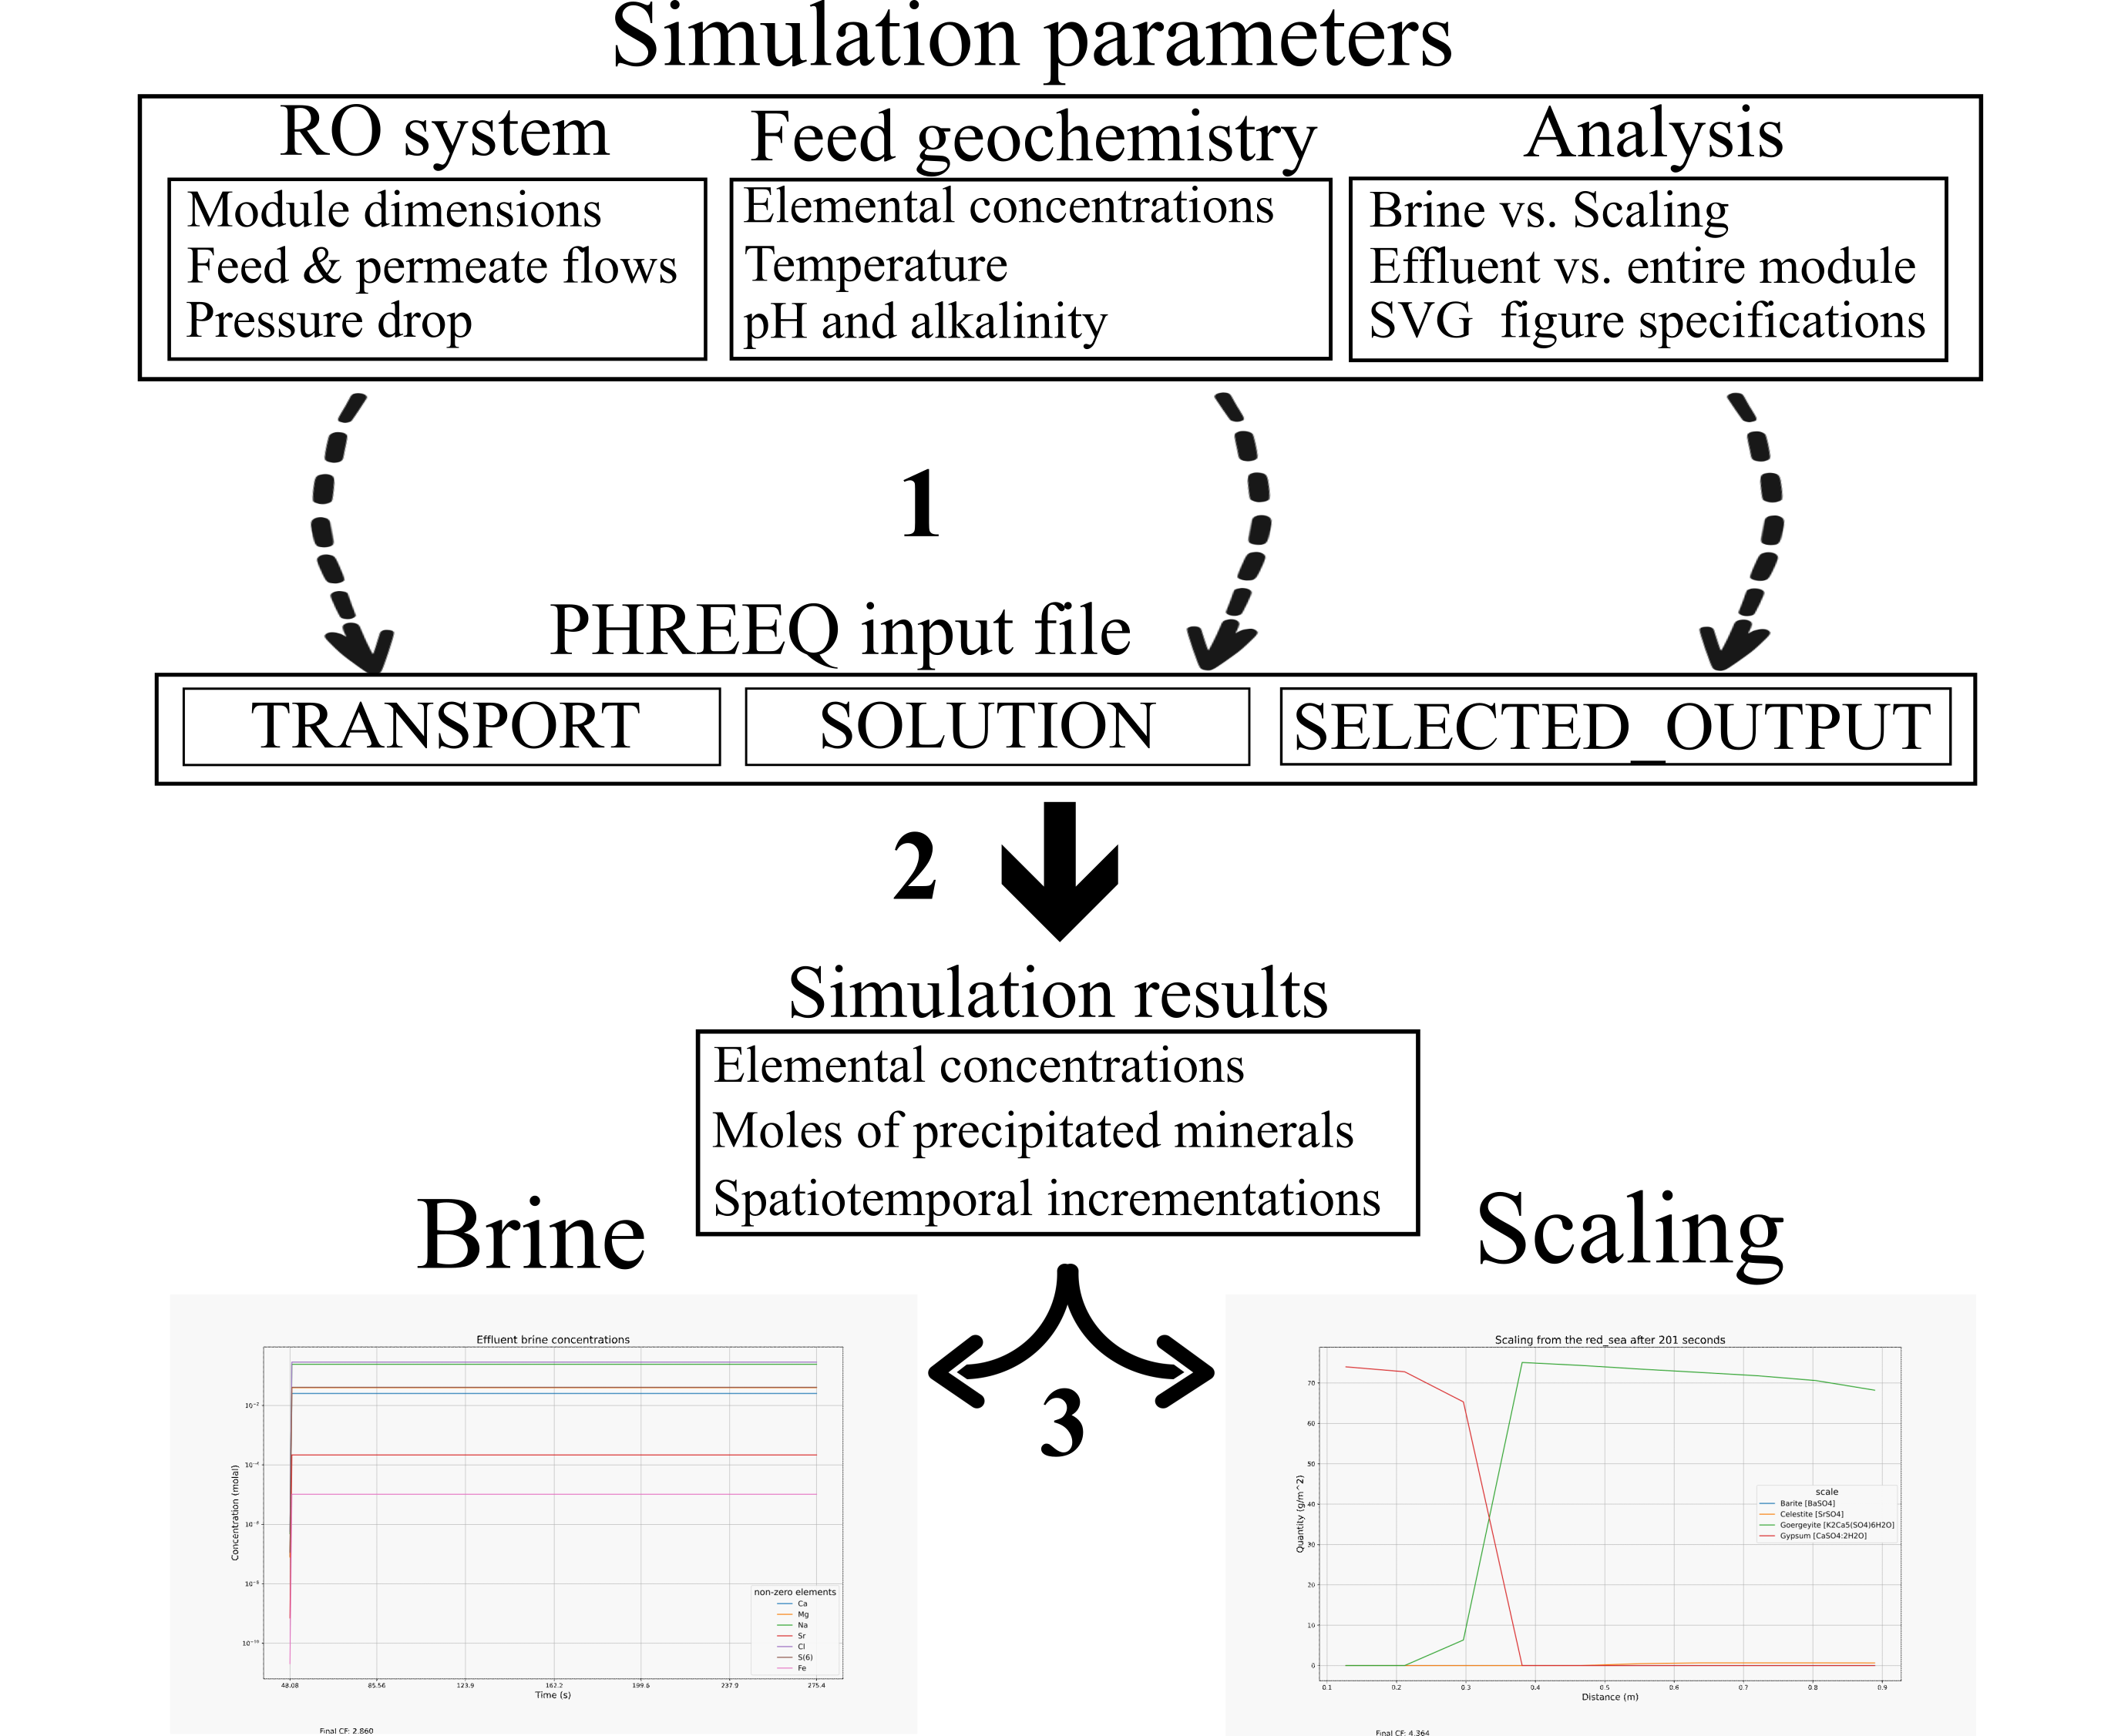
\includegraphics[width = \linewidth]{images/ROSSpy/rosspy_workflow_1.PNG}
    \caption{
        The ROSSpy workflow. Step 1 describes the translation of simulation parameters -- module specifications, feed geochemistry, and simulation analysis -- into PHREEQ code -- the TRANSPORT, SOLUTION, and SELECTED\_OUTPUT blocks, respectively --  via Python logic. Step 2 describes the execution of the PHREEQ input file via either PHREEQpy in the ROSSpy API, or via the PHREEQC batch software in iROSSpy. Step 3 describes processing the predictions of brine concentrations or scaling $\frac{g}{m^2}$ into representative figures and datatables, which are exported with other simulation files.
    }
    \label{workflow}
\end{figure}


\subsection{Numerical}
The chemical and physical processes of our aforementioned reactive transport RO model are numerically implemented through calculating parameter values for PHREEQC, and then executing PHREEQC for the simulated system. The membrane-solution interface of the RO module is first discretized into $n$ equal fractions (cells) of the total module length $l_{module}$, as a numerical approach of representing the module. These processes are detailed the following sub-sections. 

\subsubsection{Reactive geochemistry}
The geochemical processes of RO are predicated upon the PHREEQC databases. These databases provide the pivotal geochemical equations and constants that fosters accurate predictions of scaling equilibria, however, they neglect to provide mineral masses, which is essential to determine the predicted $\frac{g}{m^2}$ deposition of scale from a scaling simulation. Contemporary websites and Python modules were insufficient to interpret the complex inorganic formulas of these minerals; hence, the ChemW Python package was developed as a rigorous method of calculating the molecular mass from any chemical formula that follows conventional notation, which is detailed in its API documentation. The ChemW package provides the precise molecular masses that permit scaling predictions in the conventional units of $\frac{g~scale}{m^2~membrane}$. 

The permeate flux is assumed to be 100\% water, similar to other RO models \cite{Li2012OptimalDesalination}, and it is calculated as the change in moles ($\Delta \Phi_{e}$) of feed solution in any examined cell $e$. Permeate flux is generally proportional with transmembrane pressure ($TMP$) and the difference between feed pressure $P$ and osmotic pressure $\pi$ \cite{VanWagner2009EffectPerformance,Schock1987MassModules,Lonsdale1965TransportMembranes}
\begin{equation} \label{pressure_differential}
    \Delta \Phi_{e} ~ \alpha ~ TMP = (P - \pi),
\end{equation} 
however, these pressures are not readily measured or reported; thus, we calculate the permeate flux via two comparable methods that are elaborated in the following sections.

\subsubsection{Method 1: Linear permeate flux}
One method assumes that permeate flux is linearly distributed along the RO module according to a calculated flux slope
\begin{equation} \label{flux_slope}
    slope = \frac{(\Delta \Phi_{n}-\Delta \Phi_{1})}{n}
\end{equation}
between the first cell $1$ and the last cell $n$. The permeate fluxes in each of these border cell, $\Delta \Phi_{1}$ and $\Delta \Phi_{n}$, are calculated through a system of equations. One of these equation 
\begin{equation} \label{average_permeate_flux}
     \overbar{\Delta \Phi}_{e} = \frac{\Delta \Phi_{module}}{n} = \frac{\Delta \Phi_{n} + \Delta \Phi_{1}}{2}
\end{equation}
equates a two definitions of the average permeate flux per cell $e$: 1) ($\overbar{\Delta \Phi}_{e} = \frac{\Delta \Phi_{module}}{n}$) from the total permeate flux in the module $\Delta \Phi_{module}$, and 2) ($\frac{\Delta \Phi_{n} + \Delta \Phi_{1}}{2}$), as the average between the border cells. The other equations is the definition of relative pressure head loss \cite{Srivathsan2014ReverseUnsteadiness,Gu2020ModelingNetworks} ($HL ; 0\le HL\le 1$) across the RO module \cite{Fraidenraich2009ReverseExperiment},
\begin{equation} \label{head_loss}
     \Delta \Phi_{n}= \Delta \Phi_{1}*HL,
\end{equation}
as opposed to absolute pressure loss calculations via Darcy's law \cite{Strubbe2018CalibrationFull-Scale}, which causes $\Delta \Phi_{n}<\Delta \Phi_{1}$ per \cref{pressure_differential} as the pressure differential diminishes across the module distance \cite{Li2016Three-dimensionalChannel}. The substitution of \cref{head_loss} into \cref{average_permeate_flux} permits calculating $\Delta \Phi_{1}$ and  $\Delta \Phi_{n}$, the flux slope of \cref{flux_slope}, and subsequently $\Delta \Phi_{e}$
\begin{equation} \label{intermediary_permeate_flux}
    \Delta \Phi_{e} = (slope*e+\Delta \Phi_{1}).
\end{equation}
% Our permeate efficiency parameter ($PE; 0<PE<1$) applies here as means of considering module inefficiencies like preexisting fouling in the RO module that lessen the permeate flux of the system. The $PE$ scalar attenuates the total module permeate flux over the module through reducing \cref{intermediary_permeate_flux}: i.e. $\Delta \Phi_{old~module} = \Delta \Phi_{new~module}*PE$; $PE=0$ leads to $\Delta \Phi_{e}=0 ~\forall~ e$; and $PE=HL=1$ leads to $\overbar{\Delta \Phi}_{e}=\Delta \Phi_{e} ~\forall~ e$.

The calculation sequence for this permeate flux method is summarized:
\begin{enumerate}
    \item Parameterize the module permeate flux [$\Delta \Phi_{module}$, via the \pyobject{transport()} function]
    \item Calculate the permeate flux slope [\cref{flux_slope,average_permeate_flux,head_loss}]
    \item Calculate the permeate flux in each cell $e$ [\cref{intermediary_permeate_flux}]
\end{enumerate}


\subsubsection{Method 2: Linear Concentration Factor}
The second method assumes that the feed concentrates linearly, which causes the permeate flux to distribute non-linearly, along the RO module. The concentration factor (CF) \cite{McCaffrey1987TheHalite.,Casas2012SeawaterElectrodialysis,Kartashevsky2015PhosphateEffluents,Yan2017ReverseVelocity} can be calculated with ionic concentrations, solution masses, or permeate moles as the quotient of initial to final  \cite{Casas2012SeawaterElectrodialysis,Yan2017ReverseVelocity}
\begin{equation} \label{cf_definition}
    CF = \frac{initial}{final}
\end{equation}
as the ratio of effluent concentration to influent concentration. The CF slope in this permeate flux method is calculated analogously to \cref{flux_slope}:
\begin{equation} \label{average_cf_slope}
    slope_{CF} =\frac{CF_{n}-CF_1}{n}.
\end{equation}
The effluent $CF_{n}$ of the brine solution must be a user-defined parameter, although, it can be easily calculated as the average CF of the feed ions 
\begin{equation} \label{cf_calculation_output}
    CF_{n}=\frac{\sum_{i=1}^j(C_{i,brine})}{\sum_{i=1}^j(C_{i,feed})},
\end{equation}
where $C_{i,brine}$ is the effluent concentration and $C_{i,feed}$ is the influent concentration of ion $i$, for all $j$ ions. Defining CF from \cref{cf_definition} in terms of moles of feed ($\Phi_e$) reveals an equation 
\begin{equation} \label{cf_cell_definition}
    CF_e=\frac{\Phi_0}{\Phi_e}=\frac{\Phi_0}{\Phi_0-\Delta \Phi_{(1,e)}}
\end{equation}
that can calculate the $\Phi_e$ moles of feed at the end of cell $e$, where $\Phi_e$ equates the initial $\Phi_0$ moles of feed minus the sum of permeate flux that occurred between cell $1$ and the end of cell $e$, which can be separated
\begin{equation} \label{moles_removed_to_cell}
    \Delta \Phi_{(1,e)}=\Delta \Phi_{e}+\Delta \Phi_{(1,e-1)}
\end{equation}
into the sum of permeate flux before the start of cell $e$ ($\Delta \Phi_{(1,e-1)}=\sum_{j=1}^{e-1}(\Delta \Phi_{j})$) and the permeate flux over cell $e$ ($\Delta \Phi_{e}$). The initial $\Phi_0$ moles of feed derives from the maximal feed capacity of the simulated module,
\begin{equation} \label{feed_mass}
    \Phi_0=V_{feed}*MW_{H_2O}*\rho_{H_2O},
\end{equation}
where the feed channel volume $V_{feed}$ is calculated from the product of the module length $l_{module}$ and the cross-sectional area of the feed channel $A_{feed}$, where
\begin{equation} \label{feed_area}
    A_{feed}=(A_{module}-A_{permeate})*\frac{th_{feed}}{th_{unit}}
\end{equation}
with the cross-sectional area of the module $A_{module}$; the cross-sectional area of the permeate tube $A_{permeate}$; the thickness of the feed channel $th_{feed}$; and the thickness of the repeating membrane unit $th_{unit}$ in Figure S1. The linear expression for $CF_e$ 
\begin{equation} \label{cf_permeate_flux}
    CF_e=(slope_{CF})*e+CF_{0}~,
\end{equation}
is then substituted into \cref{cf_cell_definition}, with the slope from \cref{average_cf_slope}, to yield an expression for the permeate flux at the end of the examined cell $e$,
\begin{equation} \label{moles_removal_per_cell} 
    -\Delta \Phi_{(1,e)}=\frac{\Phi_0}{((\frac{CF_{n}-CF_{0}}{n})*e+CF_{0})}-\Phi_0~,
\end{equation}
which can be substituted into \cref{moles_removed_to_cell} with the sum of previous permeate fluxes ($\Delta \Phi_{(1,e-1)}$) to yield the permeate flux over any examined cell $e$ ($\Delta \Phi_{e}$), analogously to \cref{intermediary_permeate_flux}. Note that $\Delta \Phi_{(1,e-1)}=0$ when $e=1$, since there are no previous cells. 

The calculation sequence for this permeate flux method is summarized:
\begin{enumerate}
    \item Parameterize the effluent CF [via the \pyobject{reactions()} function]
    \item Calculate the feed capacity of the module [\cref{feed_mass,feed_area}]
    \item Calculate the CF slope [\cref{average_cf_slope}]
    \item Calculate the permeate flux in each cell [\cref{cf_cell_definition,moles_removed_to_cell,cf_permeate_flux,moles_removal_per_cell}]
\end{enumerate}


\subsubsection{Comparison of permeate flux methods}
Scaling predictions from the two aforementioned permeate flux methods are juxtaposed in Figure \ref{permeate_approach}. The most significant difference is observed at the mid-point of the simulated module ($0.47 m$), where the linear CF simulation predicts $0.99 \frac{gram}{m^2}$ of Gypsum scale while the linear permeate flux simulation predicts $0.0196 \frac{gram}{m^2}$ of Gypsum scale. These differences, however, are ultimately averaged-out, where the predicted quantity of scale over the entire module is identical between these two methods to 3 significant digits ($38.7 \frac{gram}{m^2}$). These methods are therefore believed to subtly affect only the distribution, and not the total quantity, of scale within a module. 

\begin{figure}[t]
    \centering
    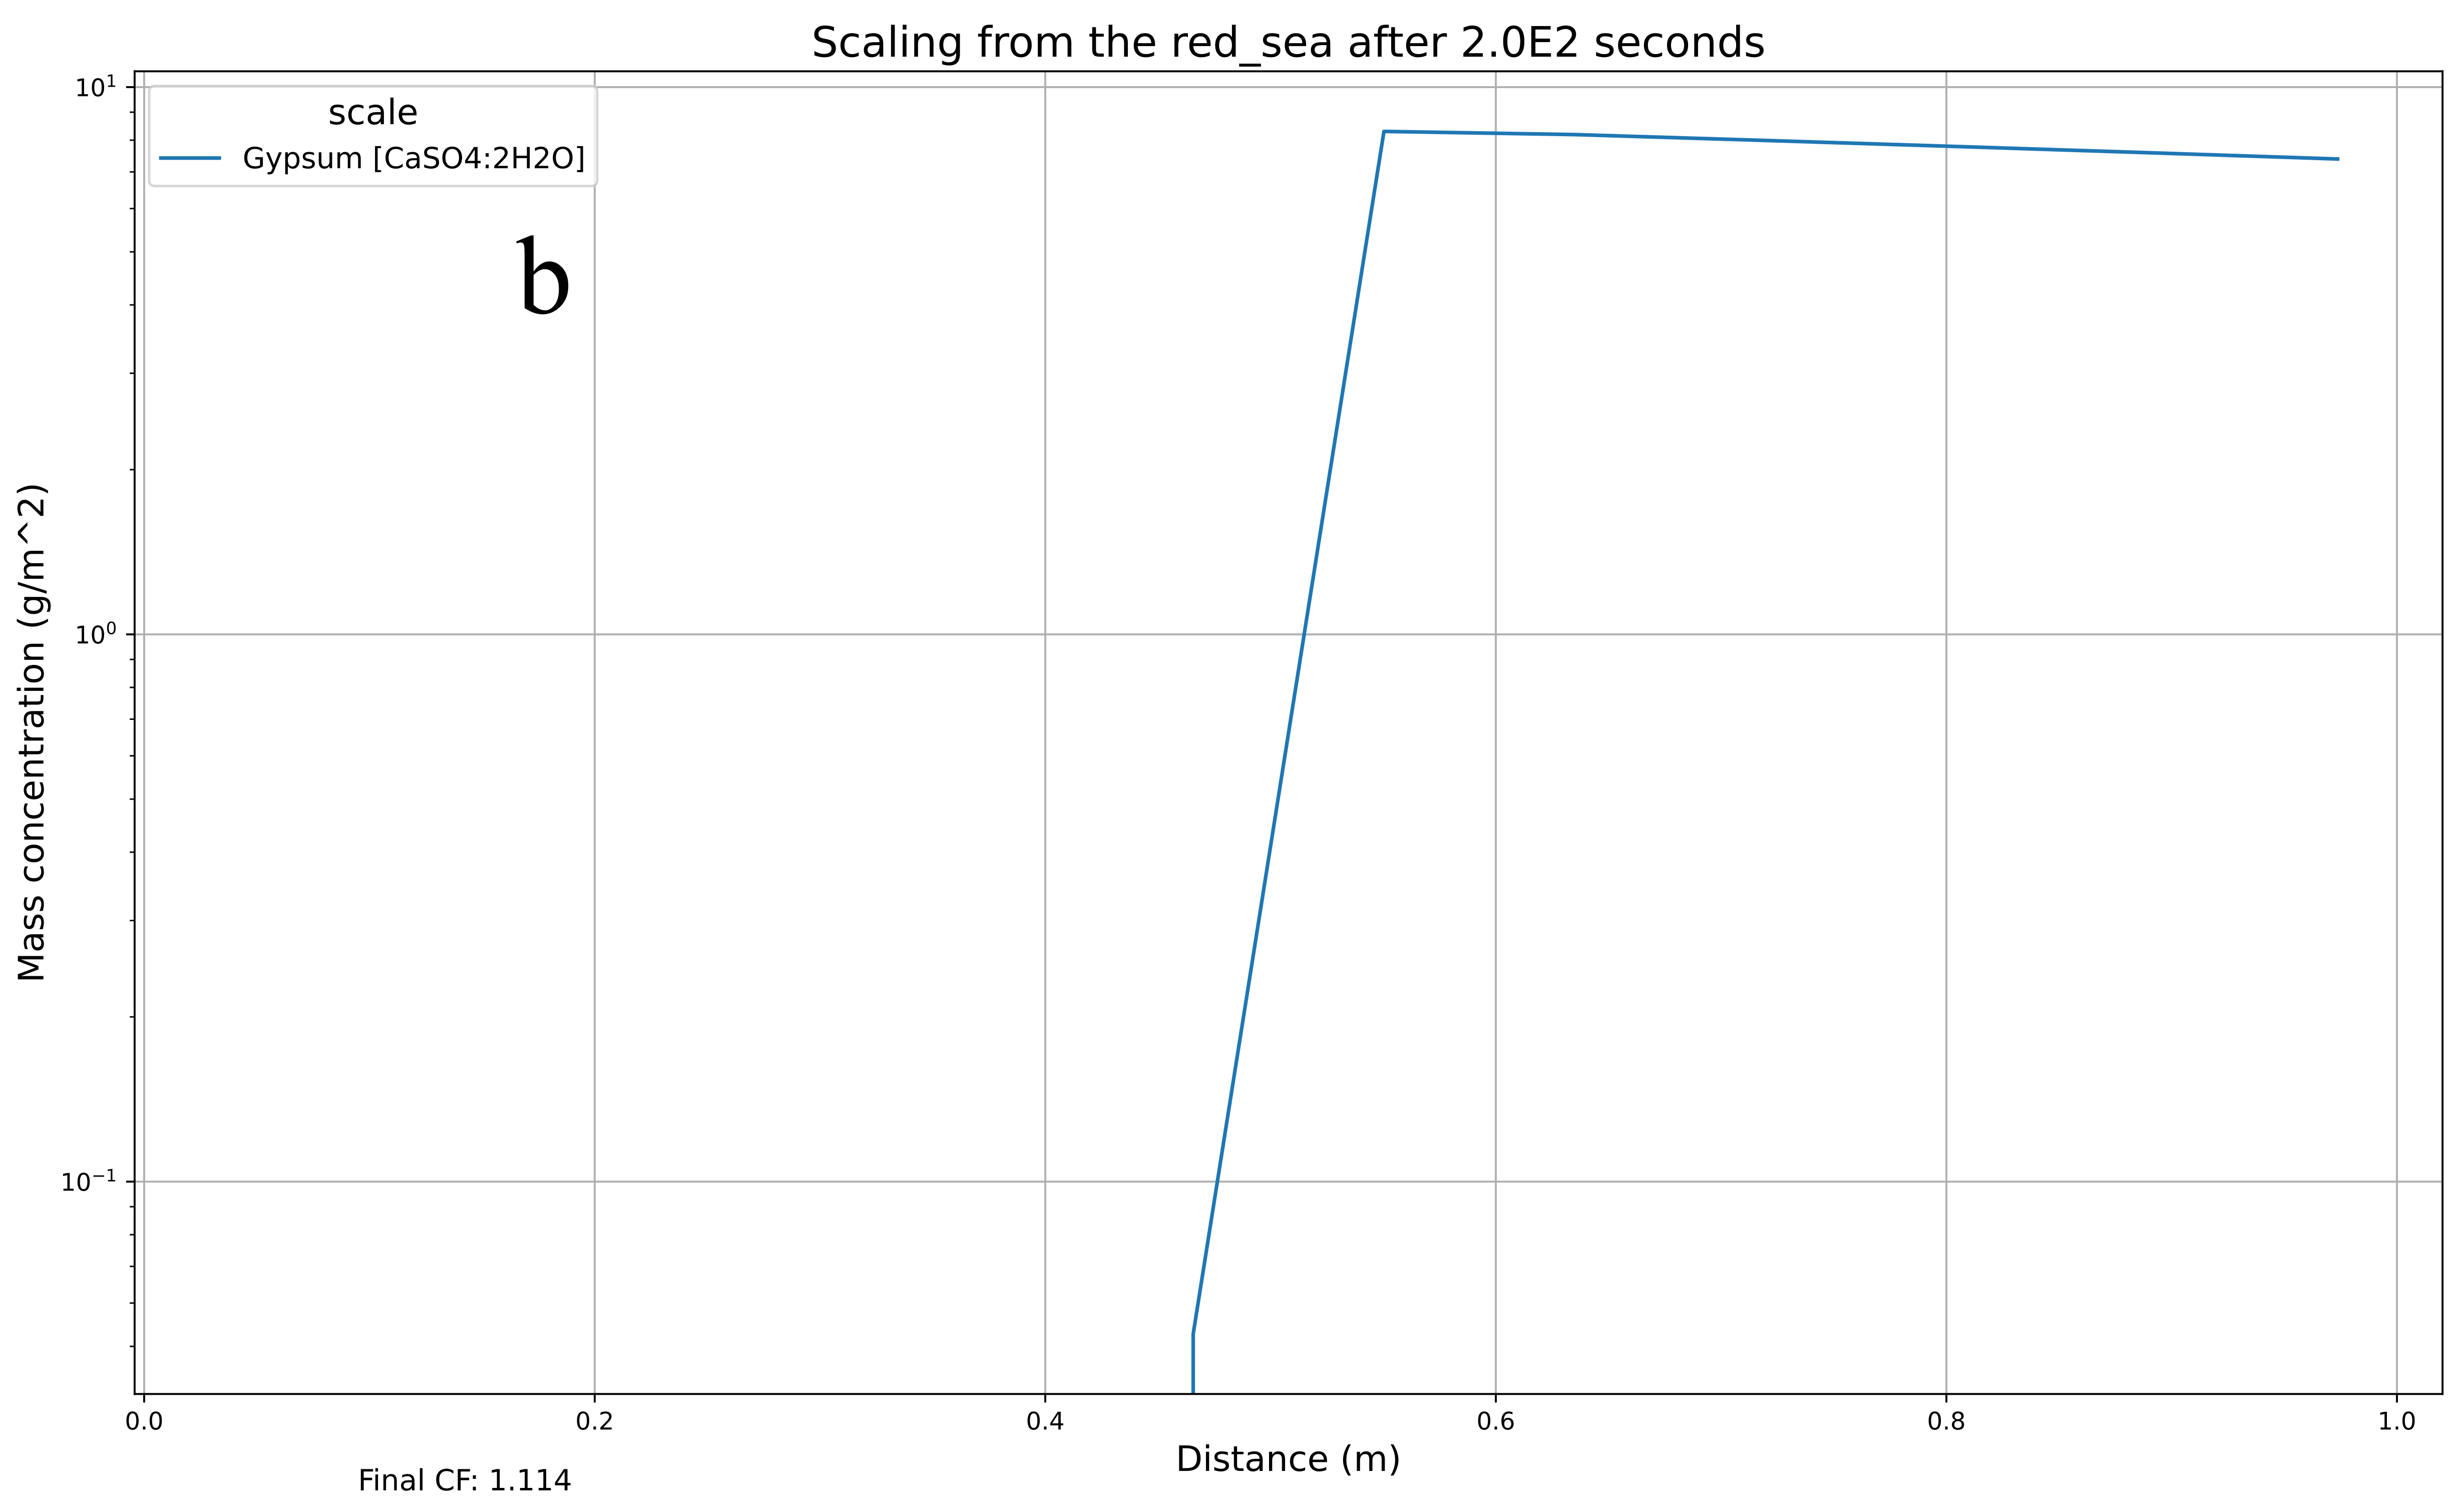
\includegraphics[width=\linewidth]{images/ROSSpy/sensitivity_analyses/permeate_approach/linear_permeate.png} \\ \midrule
    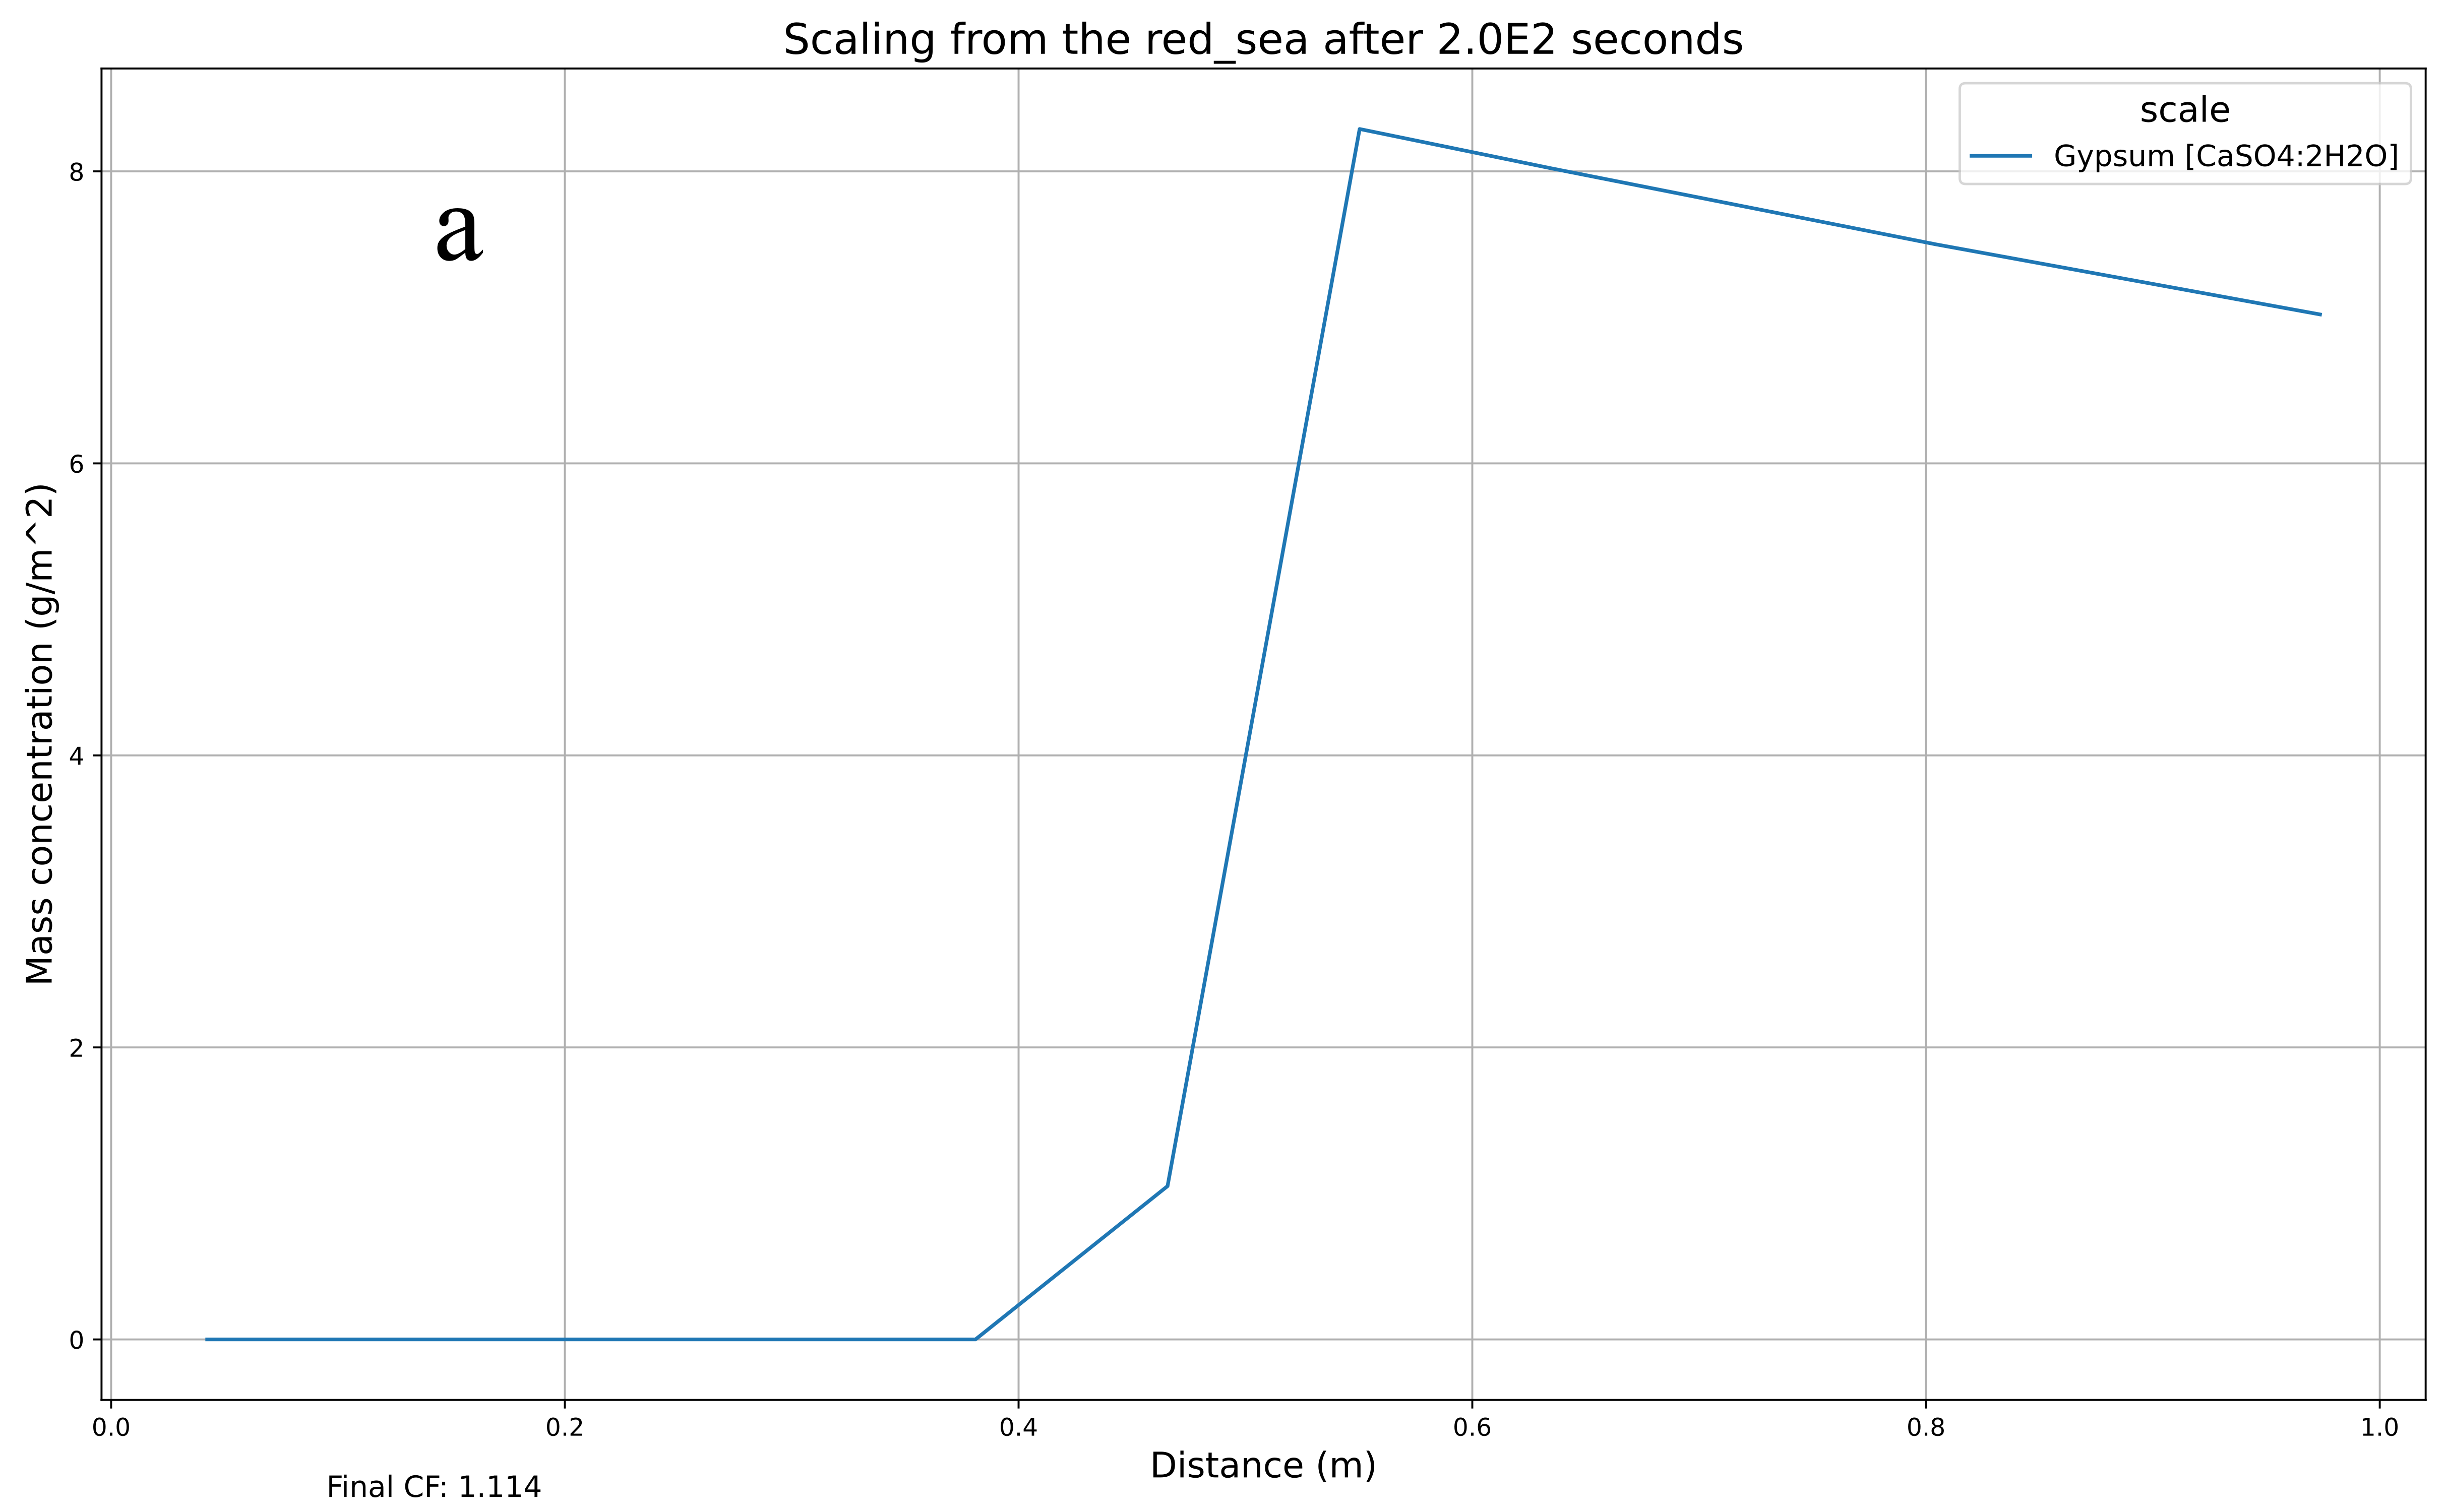
\includegraphics[width=\linewidth]{images/ROSSpy/sensitivity_analyses/permeate_approach/linear_cf.png} 
    \caption{
        Predicted scaling, of the Red Sea at $CF_{effluent}=1.114$, via the a) linear permeate flux and the b) linear CF calculation methods. 
    }
    \label{permeate_approach}
\end{figure}


\subsubsection{Transport}
The physical transport of feed through the module is simulated in each timestep by 1) migrating the contents of each cell $e$ to the next cell $e+1$ 2) repopulating cell $1$ as new feed solution enters the simulated module, and 3) deleting cell $n$ as brine exits the simulated module. The feed velocity $v_{feed}$ of the simulated module is calculated
\begin{equation} \label{feed_velocity}
    v_{feed}=\frac{Q_{max~feed}}{A_{feed}}
\end{equation}
from its maximum feed flowrate $Q_{max~feed}$ and its feed area from \cref{feed_area}. Default module parameters in Table S1, which supplement user-defined module parameters, derive from the DOW FILMTEC BW30-400 RO module like other RO models \cite{Li2012OptimalDesalination}. The maximum simulation timestep $\Delta t$ is calculated
\begin{equation} \label{timestep}
    \Delta t=\frac{l_{cell}}{v_{feed}}
\end{equation}
according to the Courant Condition \cite{Gnedin2018EnforcingSchemes} 
\begin{equation} \label{courant_condition}
    C_{max}=1 \ge \frac{v_{feed}*t_{max}}{l_{cell}}
\end{equation}
to ensure that the simulation maintains accuracy over time.

\subsection{Software}
ROSSpy combines our one-dimensional RO model with post-processing techniques. The software conducts a sequence of tasks: 1) translates user inputs into a PHREEQ input file; 2) executes the PHREEQ simulation file; 3) processes the simulation results into figures and data tables; and 4) exports all of the simulation content -- e.g. PHREEQ input file, SVGs figures, and CSVs of parameters, variables, data, and brine predictions -- into the specified folder and directory. The simulation data may be parsed and graphed according to two perspectives -- 1) all module locations in the final time or 2) all timesteps at the module end -- which may be ideal for assessing scaling or brine, respectively. The operations and syntax of ROSSpy is detailed in the API documentation.

\subsubsection{Water bodies}
Users of ROSSpy are encouraged to simulate their own feed water, which can be defined as a dictionary argument or as a JSON file. The default set of feed waters, which were assembled from experimental geochemical literature, can be simulated or they can be a syntactic model for what to include in a user-defined feed water. We propose experimental data for numerous other water sources in Section 5 of the Supporting Information that a user can adapt into feed water parameters; although, anthropogenic pollution \cite{Chen2008SourcesSea} and seasonality \cite{Sarthou2001SeasonalSea} are known to significantly alter water bodies, so direct analysis is preferable to referencing reported measurements. 

\section{Use cases}
The following sub-sections demonstrate the features of ROSSpy and the alignment of its predictions with reported measurements. These studies are detailed in Python Notebooks and simulation folders in the ROSSpy GitHub repository.

\subsection{CF and Brine formation}
The ROSSpy predictions of CF and effluent brine concentrations were verified through comparison with the following three experimental papers, where the reported feed geochemistry and module specifications were parameterized into ROSSpy. 

\paragraph{Zaman et al.\cite{Zaman2015DownstreamCompounds}}
This study  examines RO brine, from a full-scale water treatment facility in Australia, to understand which minerals are likely to form as scale. The ROSSPy predictions in Figure \ref{bar_graphs}a were $<6\%-error$ for all but one of the feed ions.

\paragraph{Ahmed et al.\cite{Ahmed2001BrineEmirates}}
This study  evaluates the RO brine from 10 small desalination plants in Oman and 8 plants in the United Arab Emirates (UAE) for the purpose of understanding ideal brine disposal methods for each brine source. We selected the UAE Qidfa I desalination plant from these 18 plants to evaluate, since it is reported more comprehensively than the other plants. The ROSSPy predictions in Figure \ref{bar_graphs}b were $<10\%-error$ for all but one of the feed ions.

\paragraph{Hajbi et al.\cite{Hajbi2010ReuseBrine}}
This study  evaluates the recovery of commodity salts from RO brine at a plant in Tunisia. The authors detail specifications of line D -- a polyamide filtration membrane -- in the plant system, in addition to the feed geochemistry, which were all parameterized into ROSSpy. The ROSSpy predictions in Figure \ref{bar_graphs}c were less aligned than the aforementioned two studies, with two ions exceeding $25\%-error$. This larger error may extend from $40\%$ fewer feed ions being defined by this study relative to the two previous studies, which creates an incomplete geochemical approximation of the feed water and thus the geochemical calculations are incorrectly skewed. 

\paragraph{CF verification}
The hypothesis of inverse proportionality between the quantity of ions in a feed source and $\%-error$ is corroborated by the accuracy of the CF prediction in the Hajbi et al. study, in the far-right columns of Figure \ref{bar_graphs}c, despite inaccurate concentration predictions. This discrepancy in accuracy between ionic concentrations and CF calculations suggests that the error resides with the geochemical calculations and not with the reactive transport that determine the CF. The accuracy of the CF in each of the studies furthermore affirms the accuracy of the reactive transport calculations for determining the permeate flux and that these calculations are evidently not the major source of error for the simulation results.

\begin{figure}[t]
    \centering
    \begin{tabular}{c|c}
        \multicolumn{2}{c}{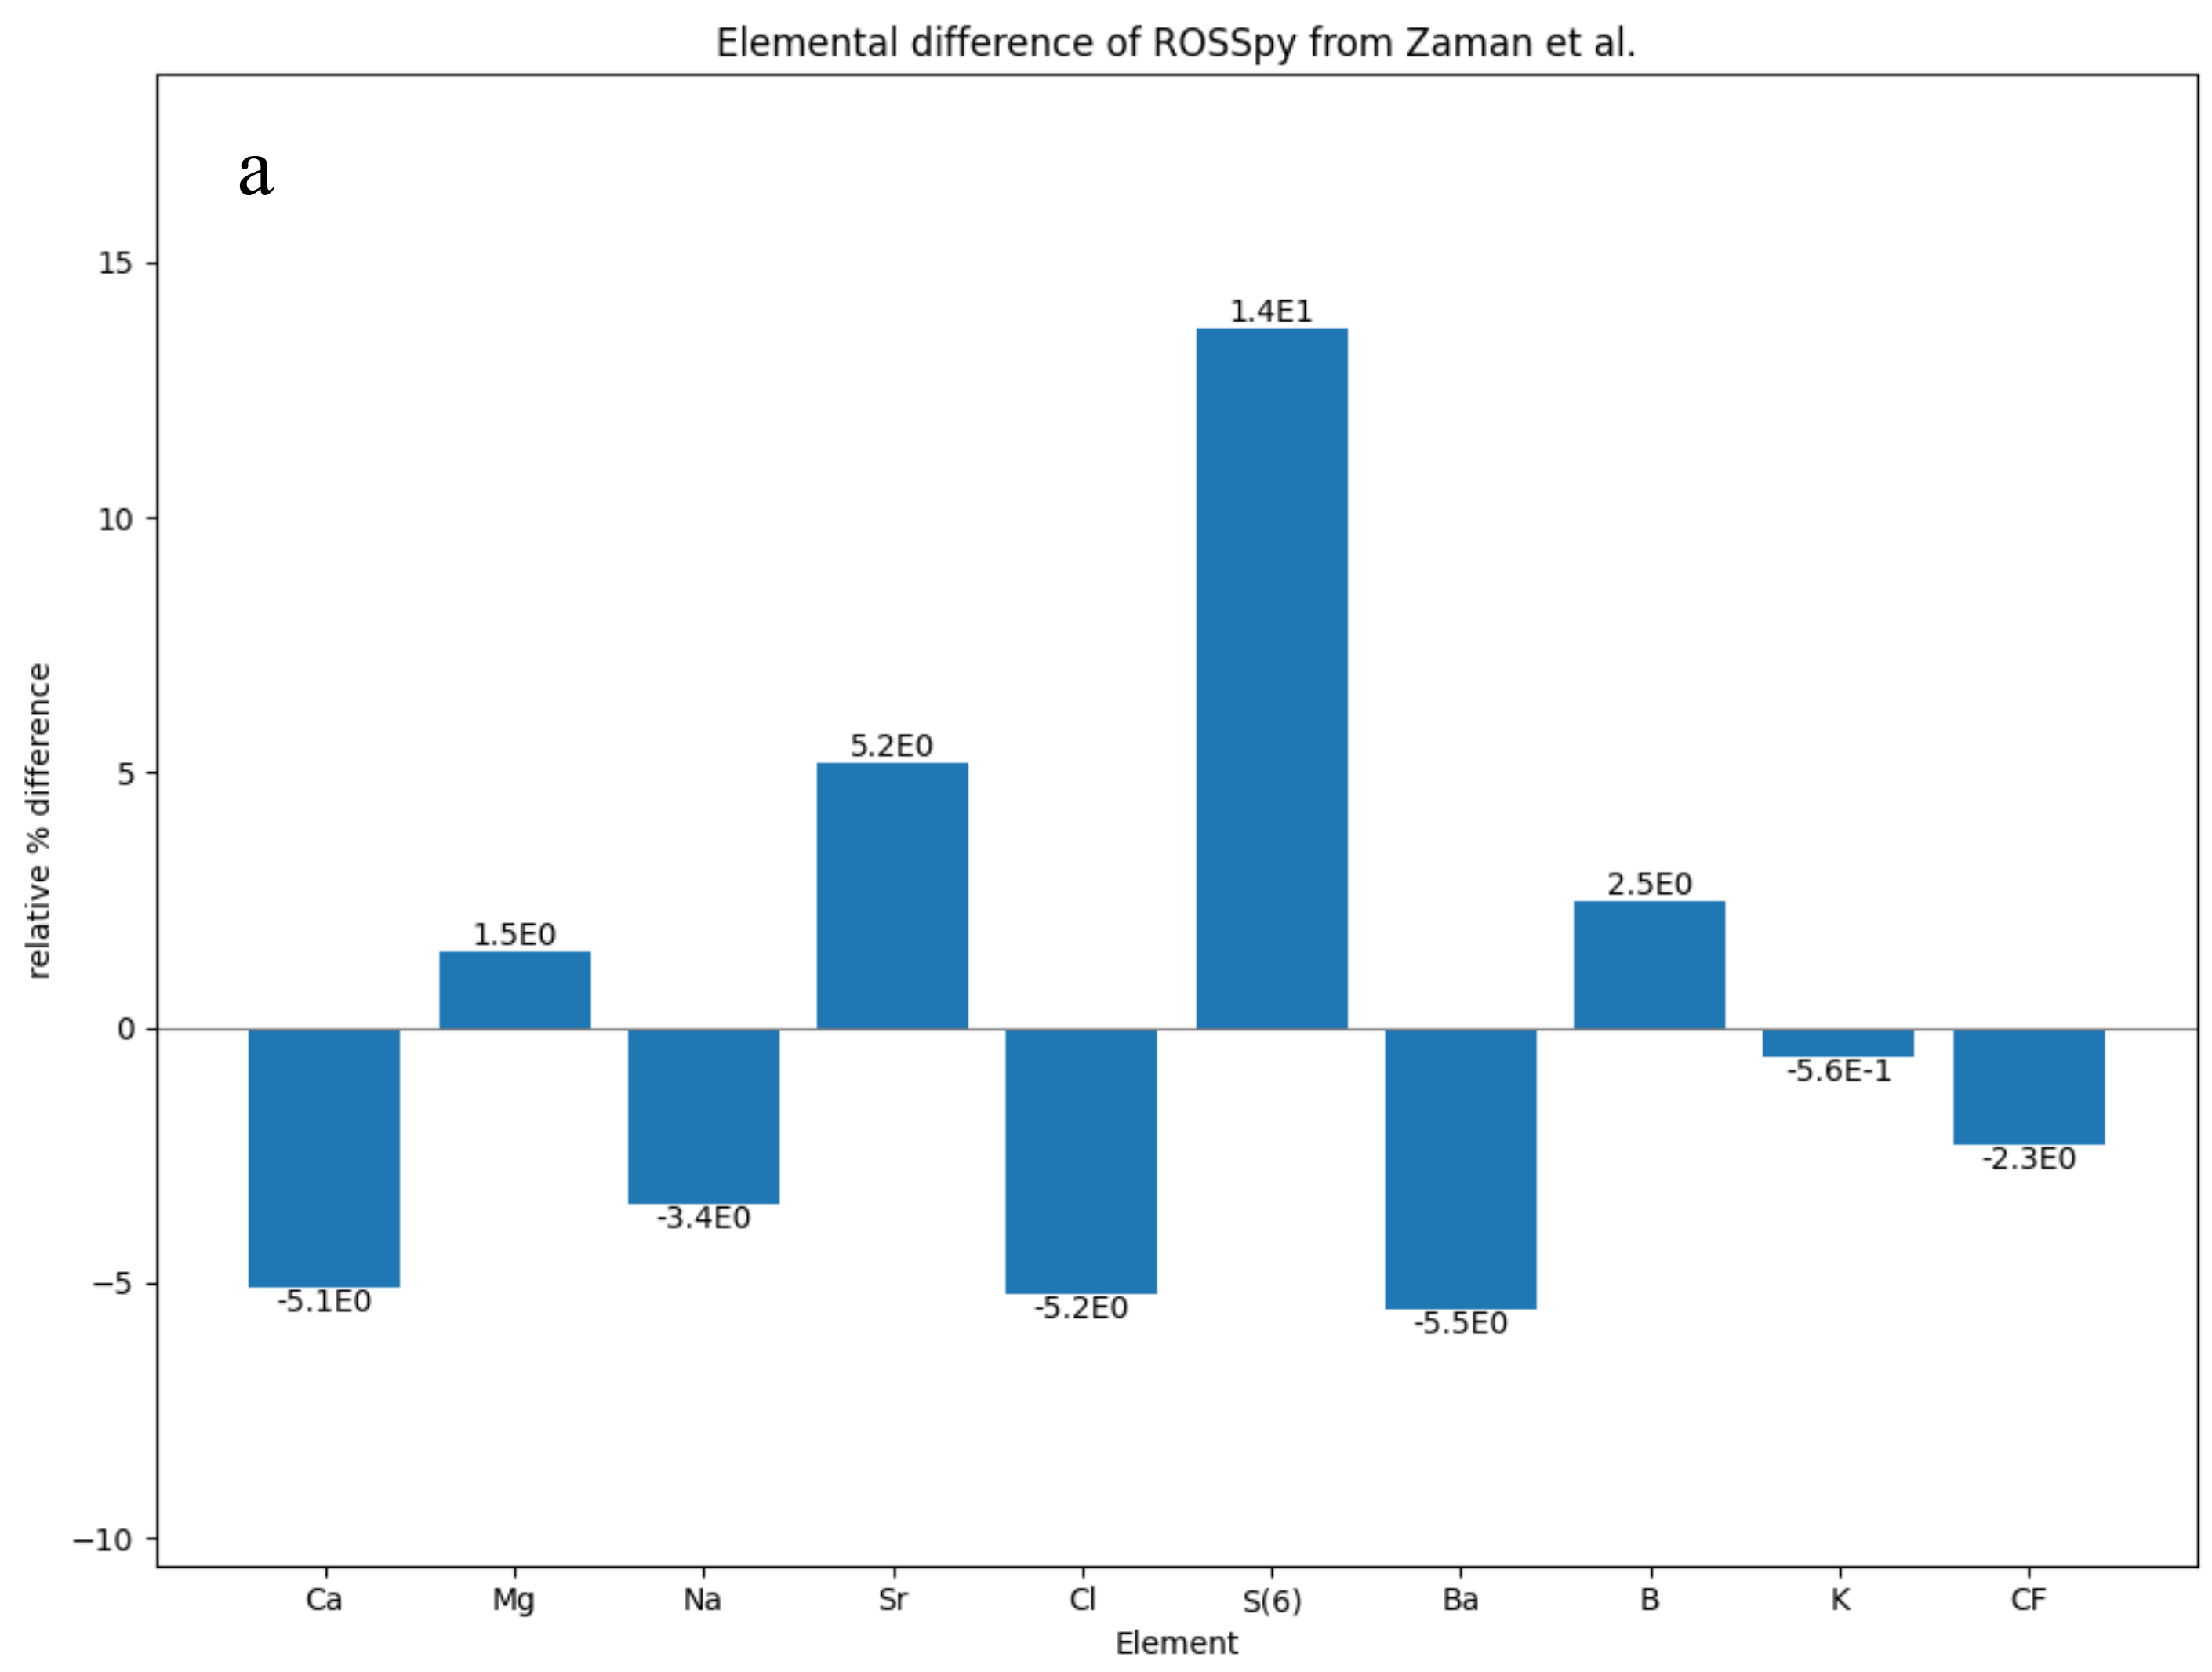
\includegraphics[width=\linewidth]{images/ROSSpy/case_studies/Zaman_comparison.png}} \\ \midrule
        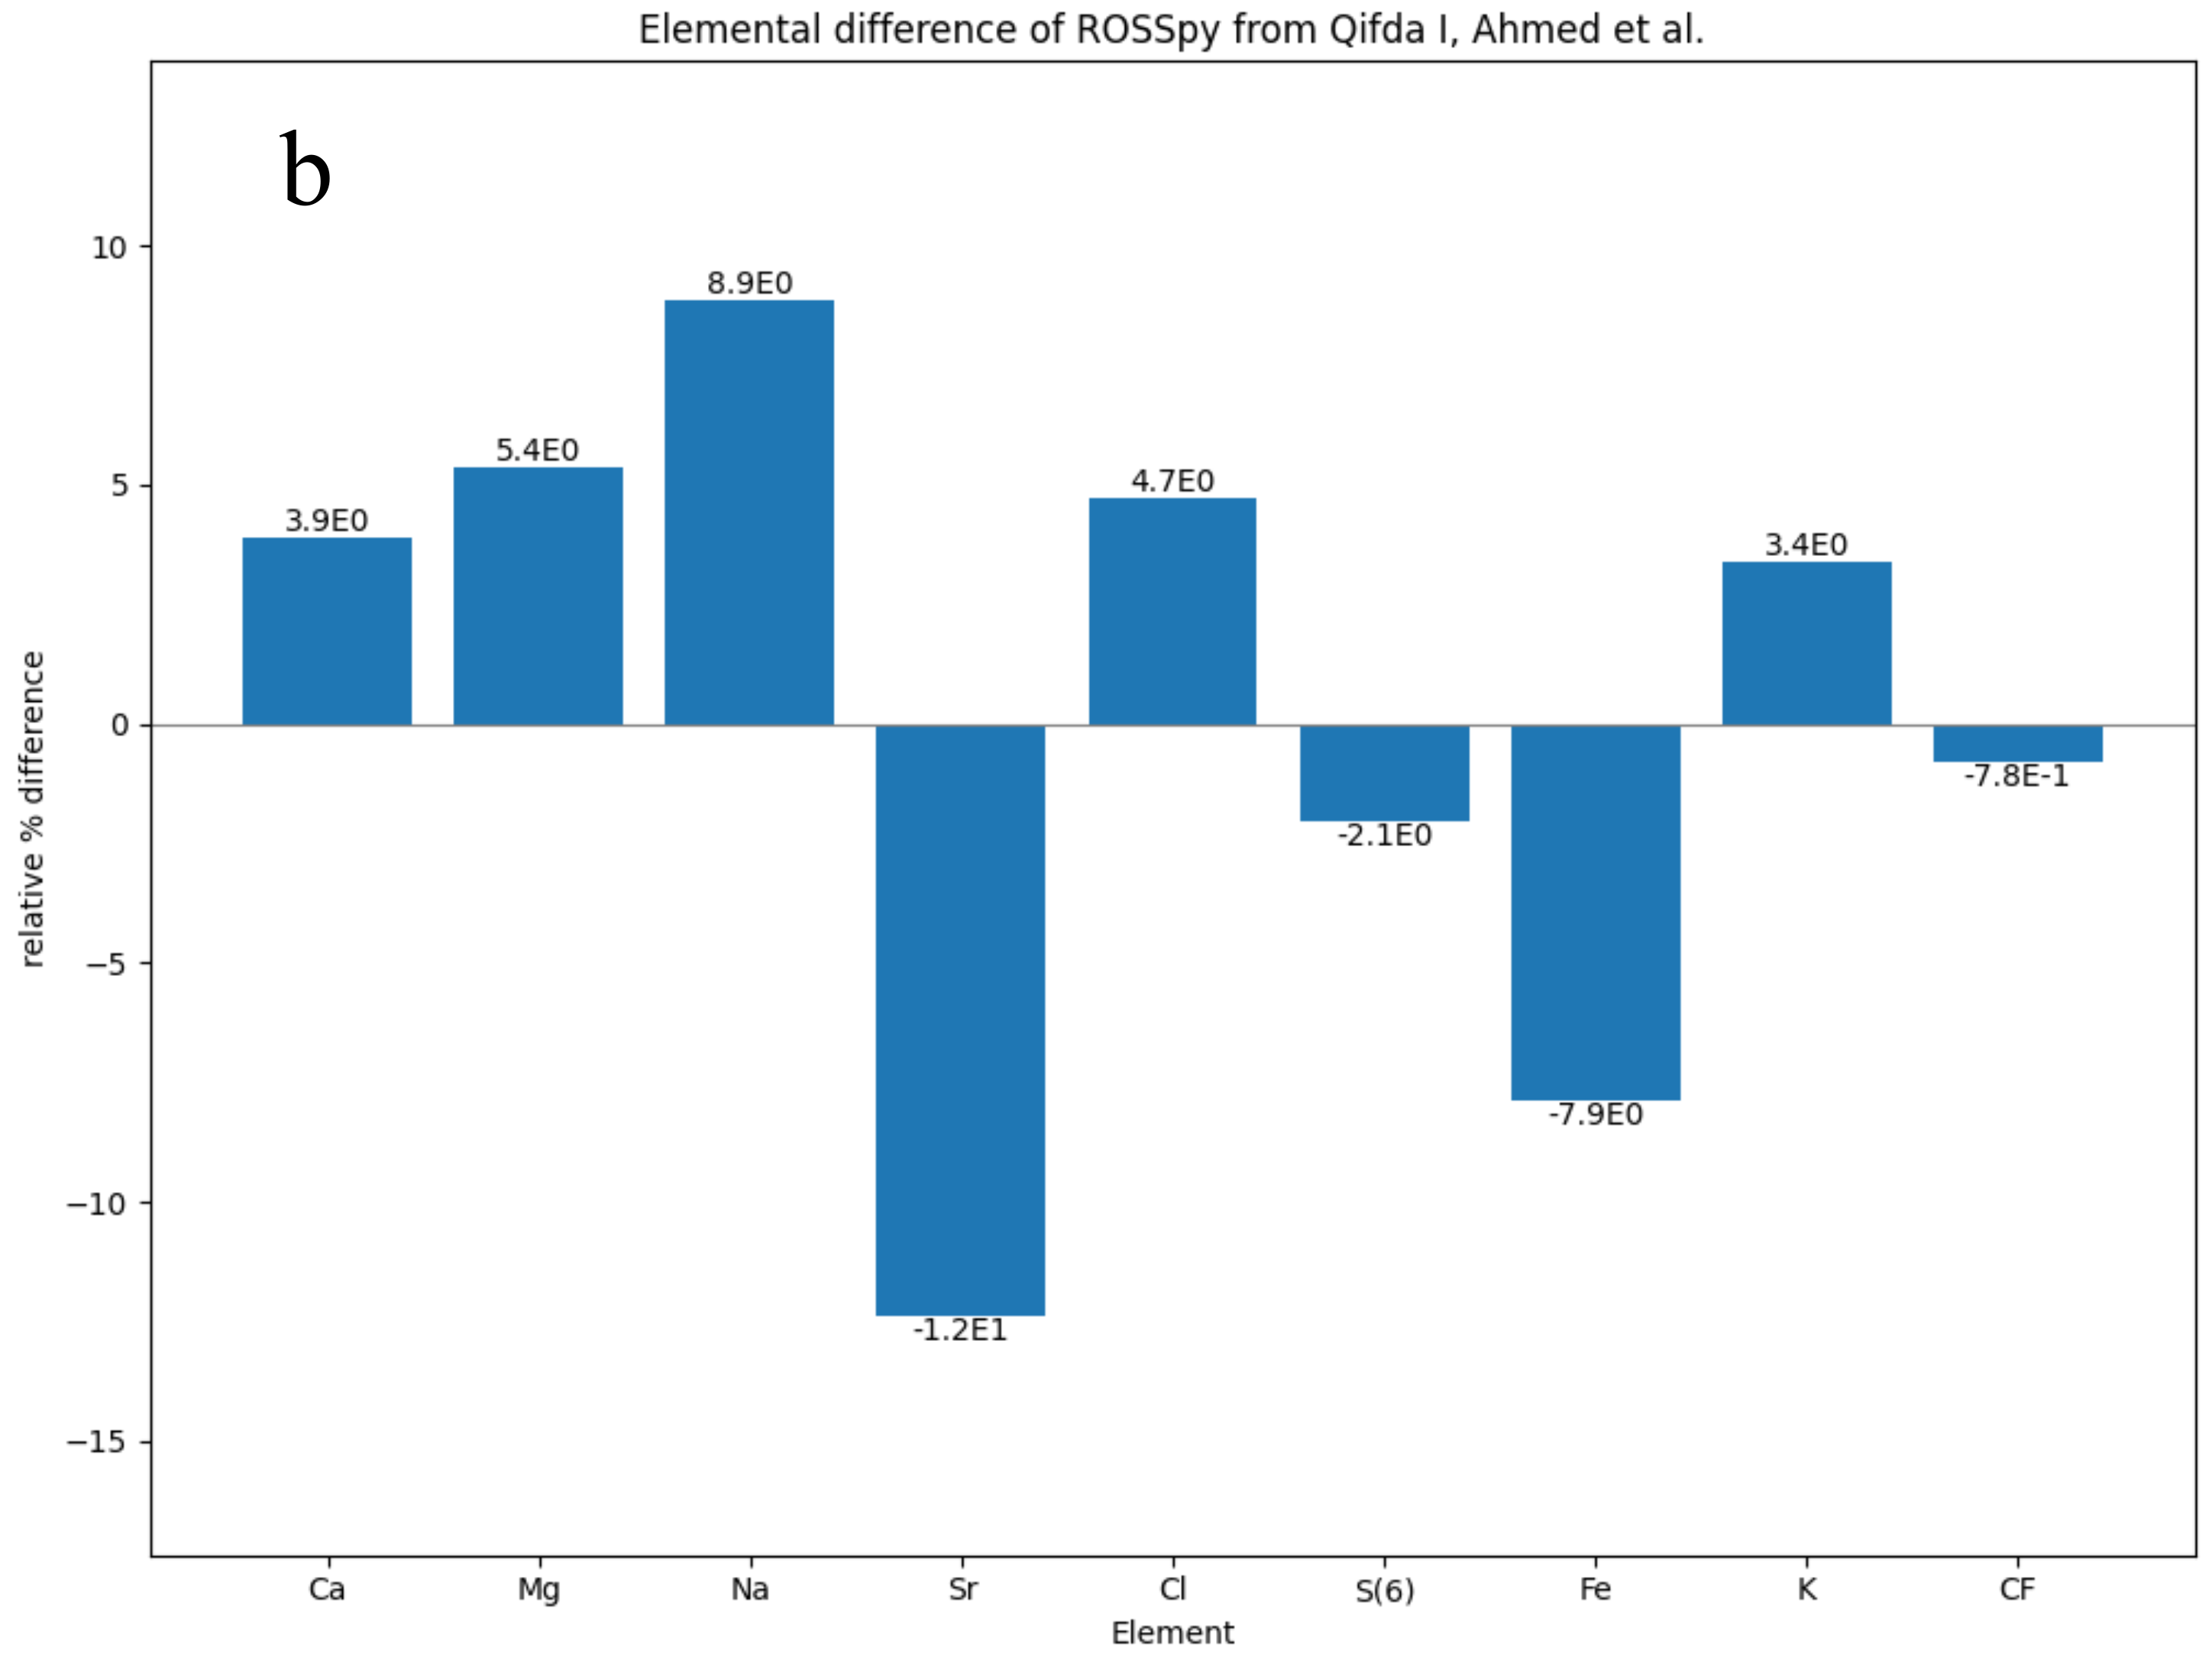
\includegraphics[width=0.49\linewidth]{images/ROSSpy/case_studies/Ahmed_comparison.png} & 
        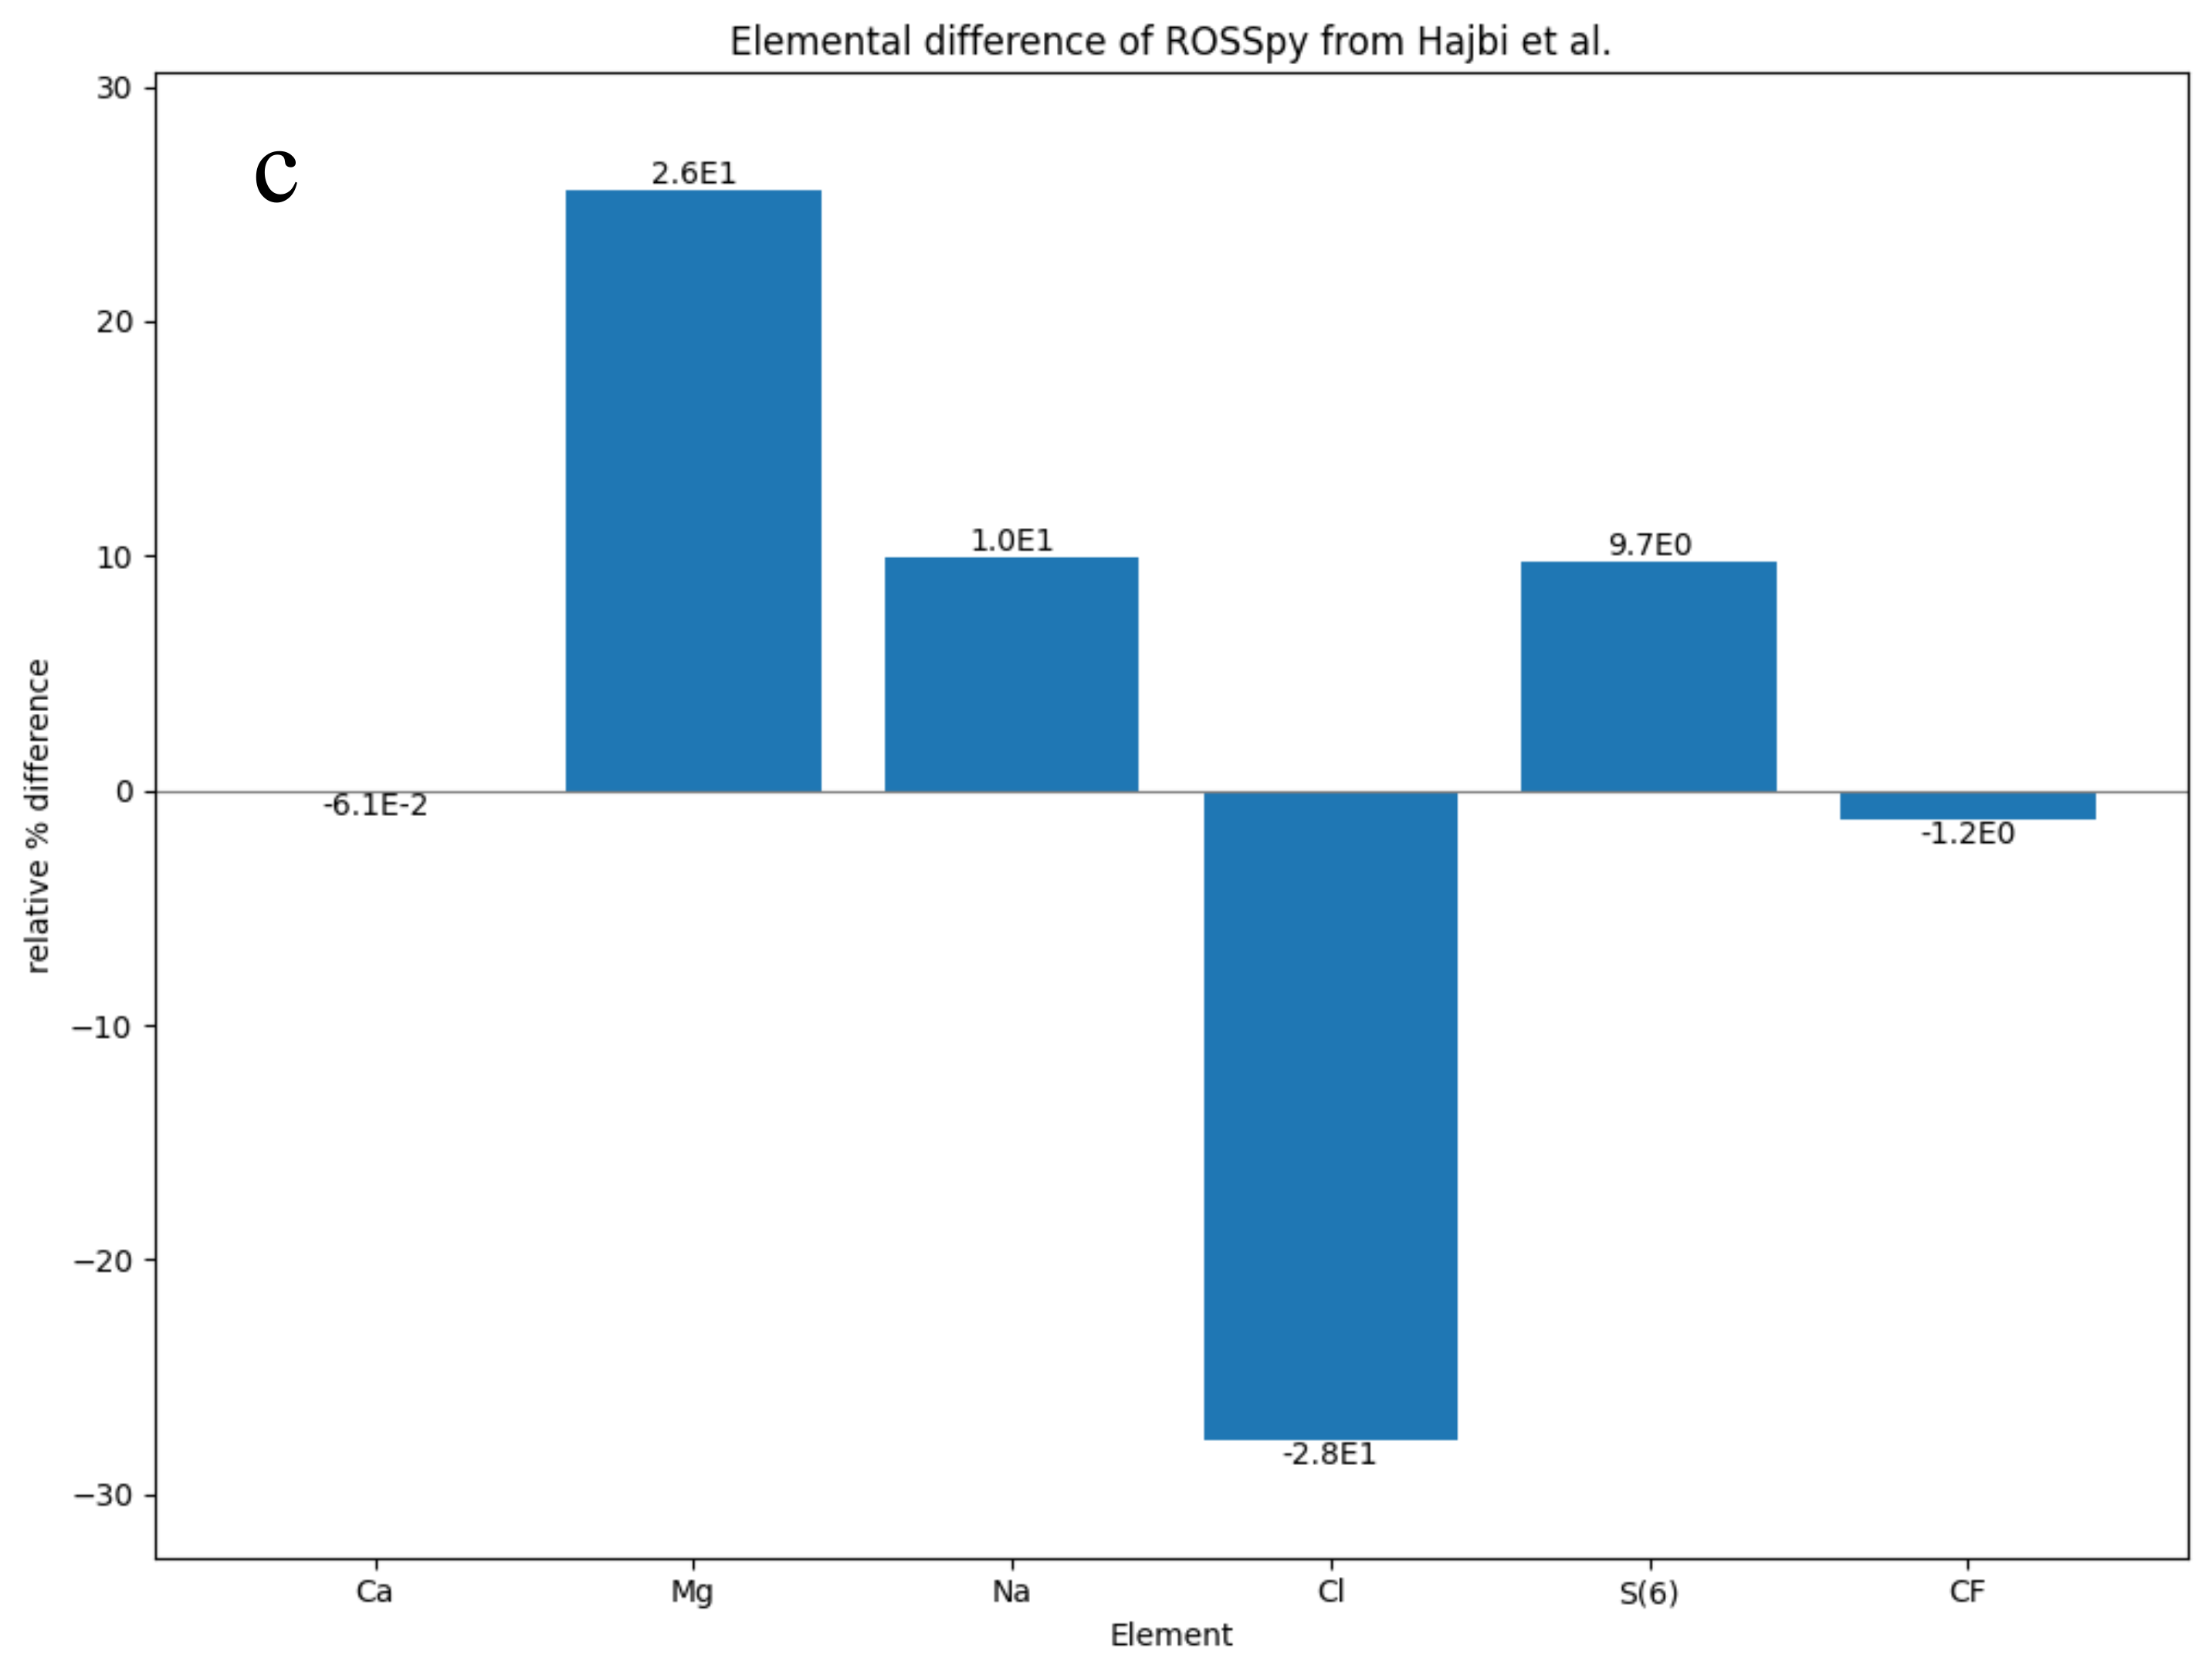
\includegraphics[width=0.49\linewidth]{images/ROSSpy/case_studies/Hajbi_comparison.png} \\ \bottomrule
    \end{tabular}
    \caption{
        The \%-error between the predicted effluent brine concentrations from ROSSpy and the experimental brine measurements from RO plants. Panels a-c) correspond with the Zaman et al. \cite{Zaman2015DownstreamCompounds}, Ahmed et al. \cite{Ahmed2001BrineEmirates}, and Hajbi et al. \cite{Hajbi2010ReuseBrine} studies, respectively, and each possess different y-axis scales to best resolve the bars in each graph. 
    }
    \label{bar_graphs}
\end{figure}


\subsection{Scaling}
The scaling predictions were verified quantitatively and qualitatively, from theoretical calculations and experimental literature, respectively. Experimental literature was not discovered that quantified scaling while also articulating the feed geochemistry that is necessary to replicate the study in ROSSpy. 

\subsubsection{Quantitative}
The precipitation equilibria of PHREEQC were quantitatively verified through an ICE table for a simple case of Gypsum precipitation. The predicted precipitation of $0.01961$ moles of Gypsum, in Table \ref{gypsum_ice_table}a, is 7\% greater than the $0.01859$ moles that is expected based upon the stoichiometry of the equilibrium reaction. This deviation is attributed to the printed PHREEQC concentrations from Table \ref{gypsum_ice_table}a only embodying advection and not embodying the solution diffusion that also influences RO reactive transport. The same $+7\%$-error was observed between the predicted precipitation of $0.194$ moles from simulating the Red Sea (solved in eq. S2) versus the expected precipitation of $0.181$ moles from a simple system of $Ca^{2+}$ and $SO_4^{2-}$ ions in Table \ref{gypsum_ice_table}b (solved in eq. S1). This deviation is attributed to ionic interactions of the Red Sea feed that are not considered in the simplified system of only $Ca^{2+}$ and $SO_4^{2-}$. These subtle 7\% deviations, notwithstanding their complexities beyond the scope of these simple ICE tables, are relatively minor in the context of other sources of error, e.g. feed measurements, and still provide close quantitative estimates of scaling.

\begin{table}
    \centering
    \begin{tabular}{c|ccccc}
      \toprule
      \textbf{a} & $Ca^{2+}$ & $+$ & $SO_4^{2-}$ & $\leftrightharpoons$ & $CaSO_4$ \\
      \midrule
      I & $0.3545$ && $1.816$ && $0$ \\
      C & $-0.01859$ && $-0.01859$ && $+0.01961$ \\
      F & $0.3360$ && $1.797$ && $0.01961$ \\
      \bottomrule
      \\
      \toprule
      \textbf{b} & $Ca^{2+}$ & $+$ & $SO_4^{2-}$ & $\leftrightharpoons$ & $CaSO_4$ \\
      \midrule
      I & $0.003913$ && $0.00633$ && $0$ \\
      C & $-x$ && $-x$ && $+x$ \\
      F & $0.003913-x$ && $0.00633-x$ && $x$ \\
      \bottomrule
    \end{tabular}
    \caption{
        Gypsum precipitation according to the ICE (Initial, Change, Equilibrium) model, except that "Equilibrium" (E) is replaced with "Final" (F) since the system never completely reaches equilibrium before the solution leaves the simulated module. The bottom ICE table estimated Gypsum precipitation after desalination -- based upon the $K_{sp}$ of Gypsum and the activity coefficients of the feed solution from iPHREEQC -- in eq. S1. 
      }
    \label{gypsum_ice_table}
\end{table}

\subsubsection{Qualitative}
The scaling predictions from ROSSpy were qualitatively verified through comparison with the following three experimental studies. 

\paragraph{Karabelas et al., 2020 \cite{Karabelas2020ScalingTools}}
This study reviews the state-of-the-art for software that predicts RO scaling, which inspired the development and features of ROSSpy, and provides in Section 7 of the Supporting Information details of feed geochemistry and module specifications for an RO desalination plant. The ROSSpy predictions in Figure \ref{qualitative_scaling}a from these parameters exactly match the reported scale observations ("Calcite but not Gypsum" and a "few other salts, such as Barite and Dolomite, could also deposit at downstream...") in numerous ways: 1) Calcite was the primary scalant; 2) Gypsum was not a predicted scalant; 3) a few other salts precipitated with lesser quantity, including Dolomite and Barite; and 4) the minor salts, primarily Dolomite, precipitated more in the downstream portion of the module.  

\paragraph{Karabelas et al., 2014 \cite{Karabelas2014IncipientChannels}}
This study elucidates the mechanisms of incipient scaling from RO desalination -- with Gypsum as the archetypal scalant \cite{Lyster2009CoupledModule,Radu2014ASystems}. The ionic concentrations of trial ID 28SC in the paper were parameterized into ROSSpy, and the only predicted scalant was Gypsum in Figure \ref{qualitative_scaling}b, which is identical to the reported results.  

\paragraph{Lee et al., 2009 \cite{Lee2009MembraneWastewater}}
This study evaluates the use of a membrane bioreactor -- which is a hollow-fiber membrane module design that is mechanistically similar to RO and thus can be represented by the same reactive transport model as RO -- to treat wastewater. The wastewater feed geochemistry was parameterized into ROSSpy, and only predicted scalant was Calcite in Figure \ref{qualitative_scaling}c, which is identical to the reported results.

\begin{figure}
    \begin{tabular}{c|c}
        \multicolumn{2}{c}{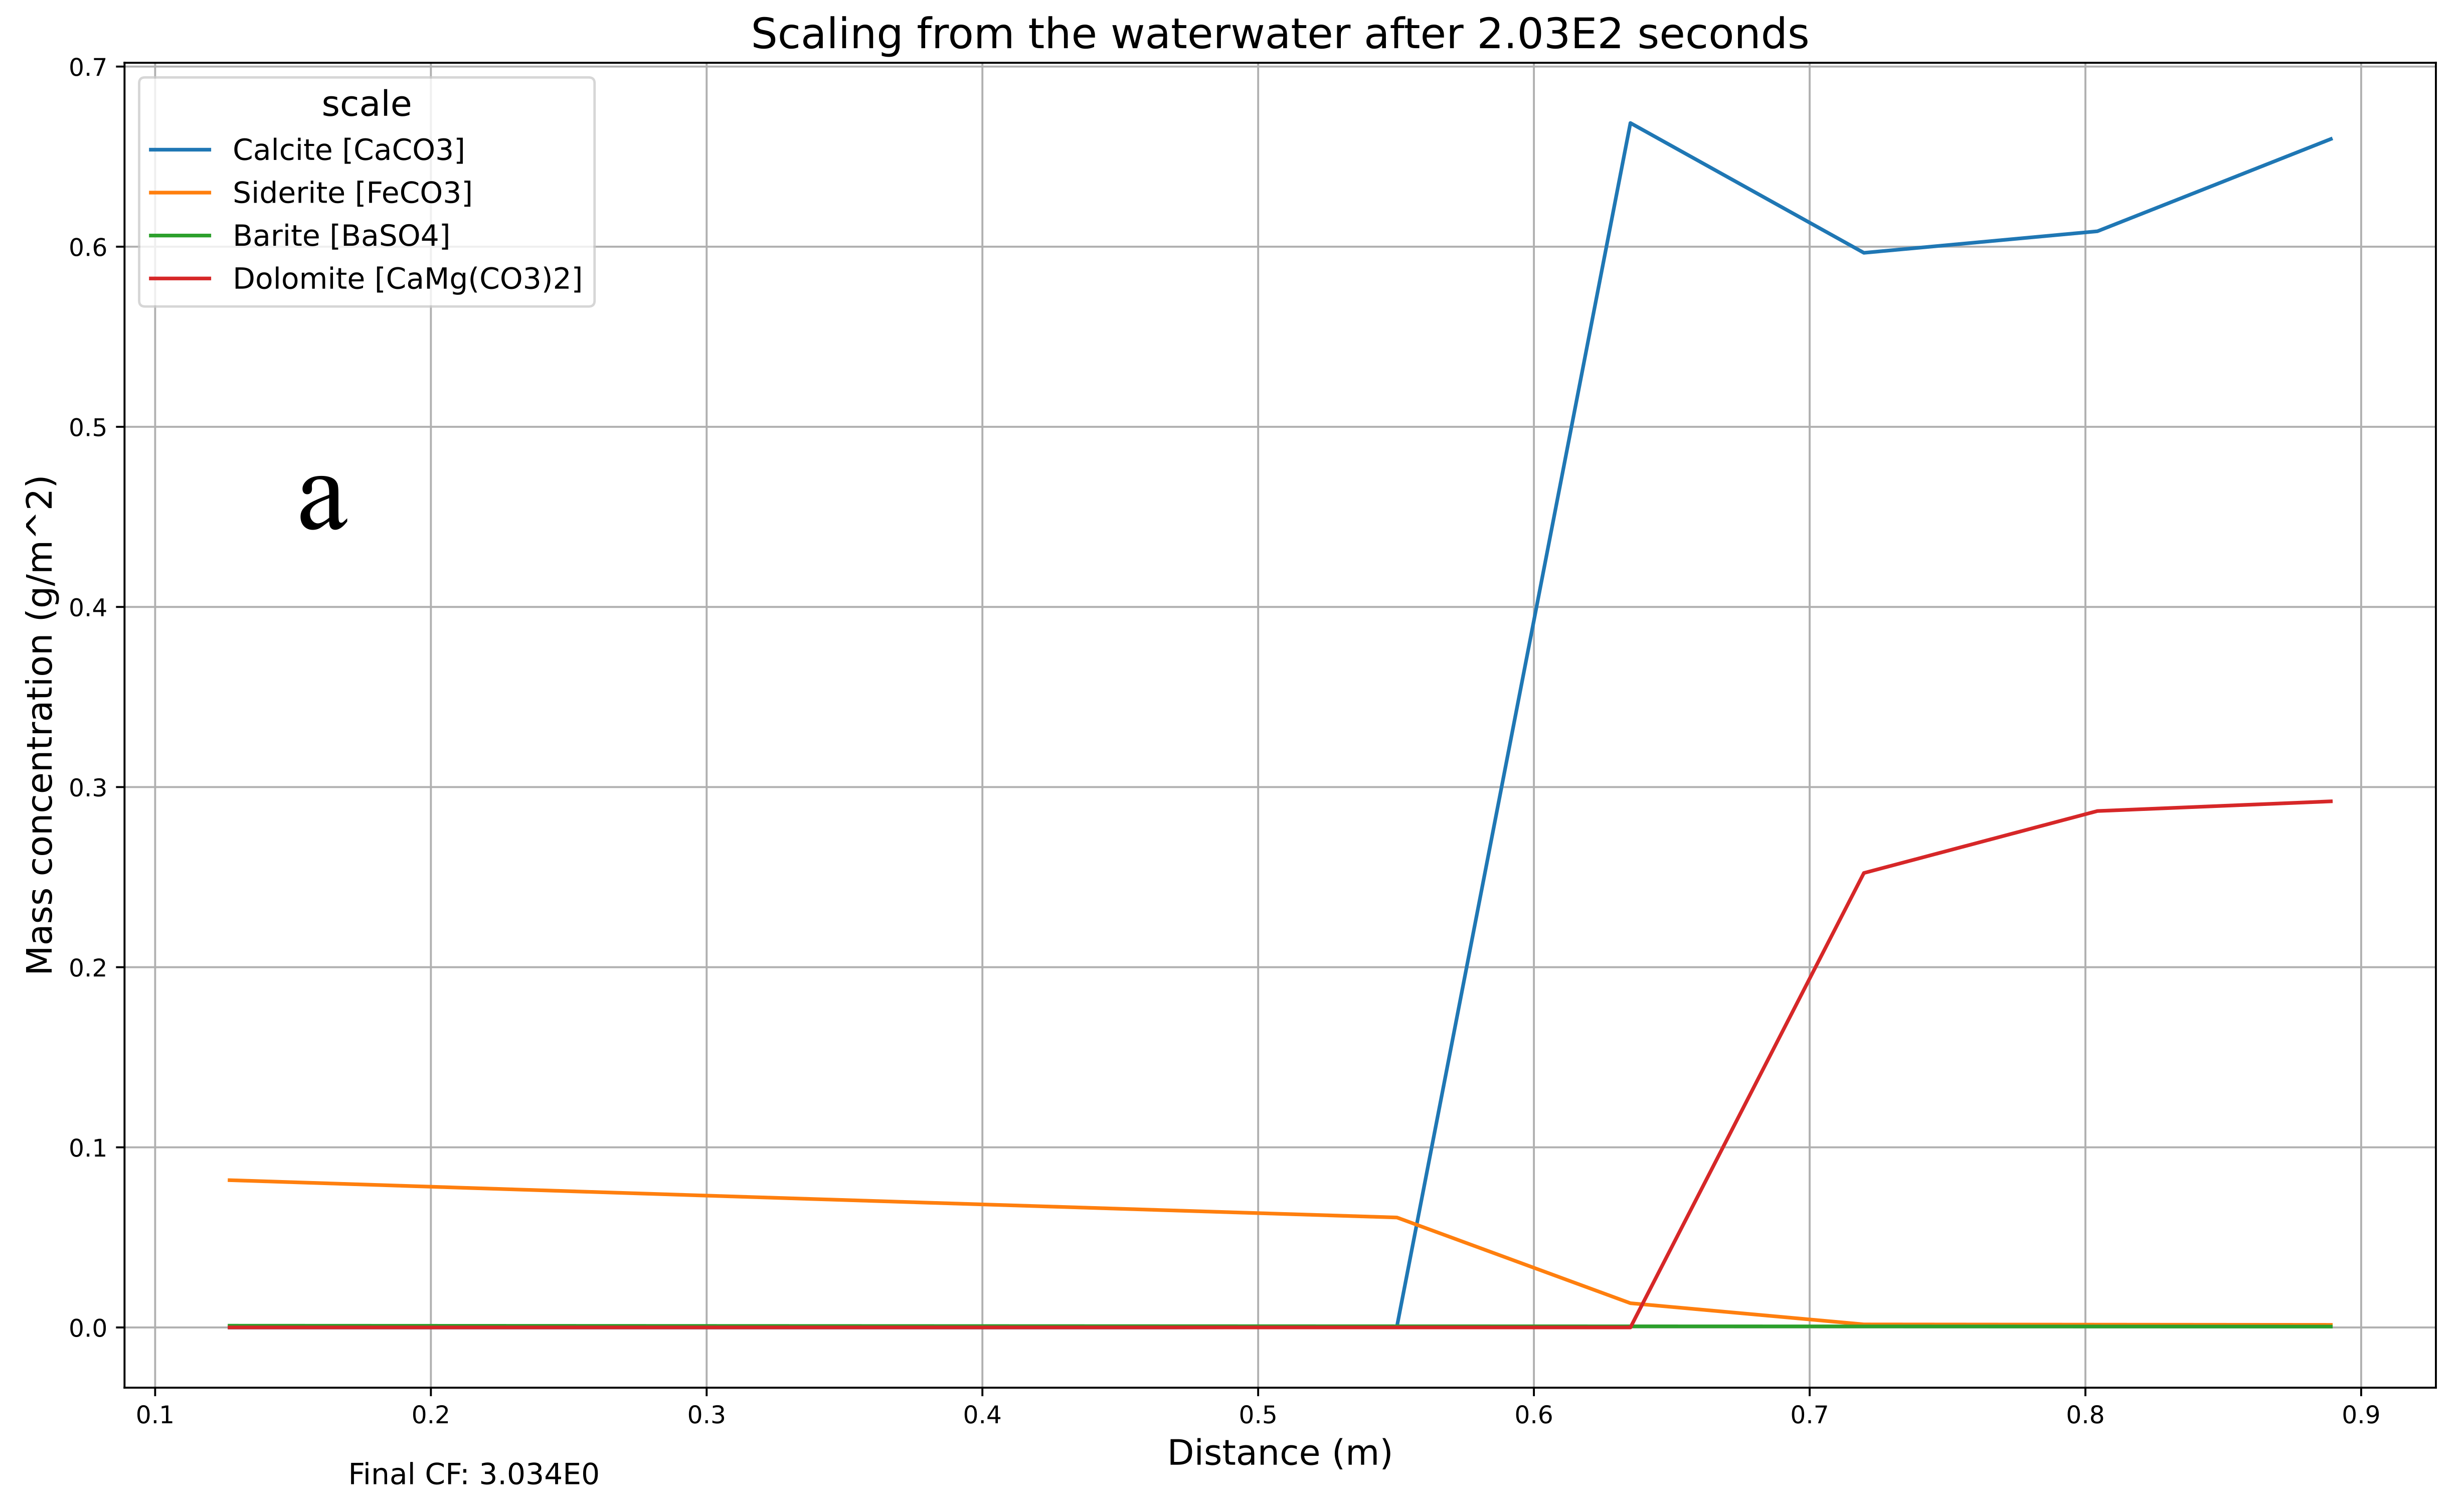
\includegraphics[width=\linewidth]{images/ROSSpy/case_studies/Karabelas_2020_wateq4.png}} \\
        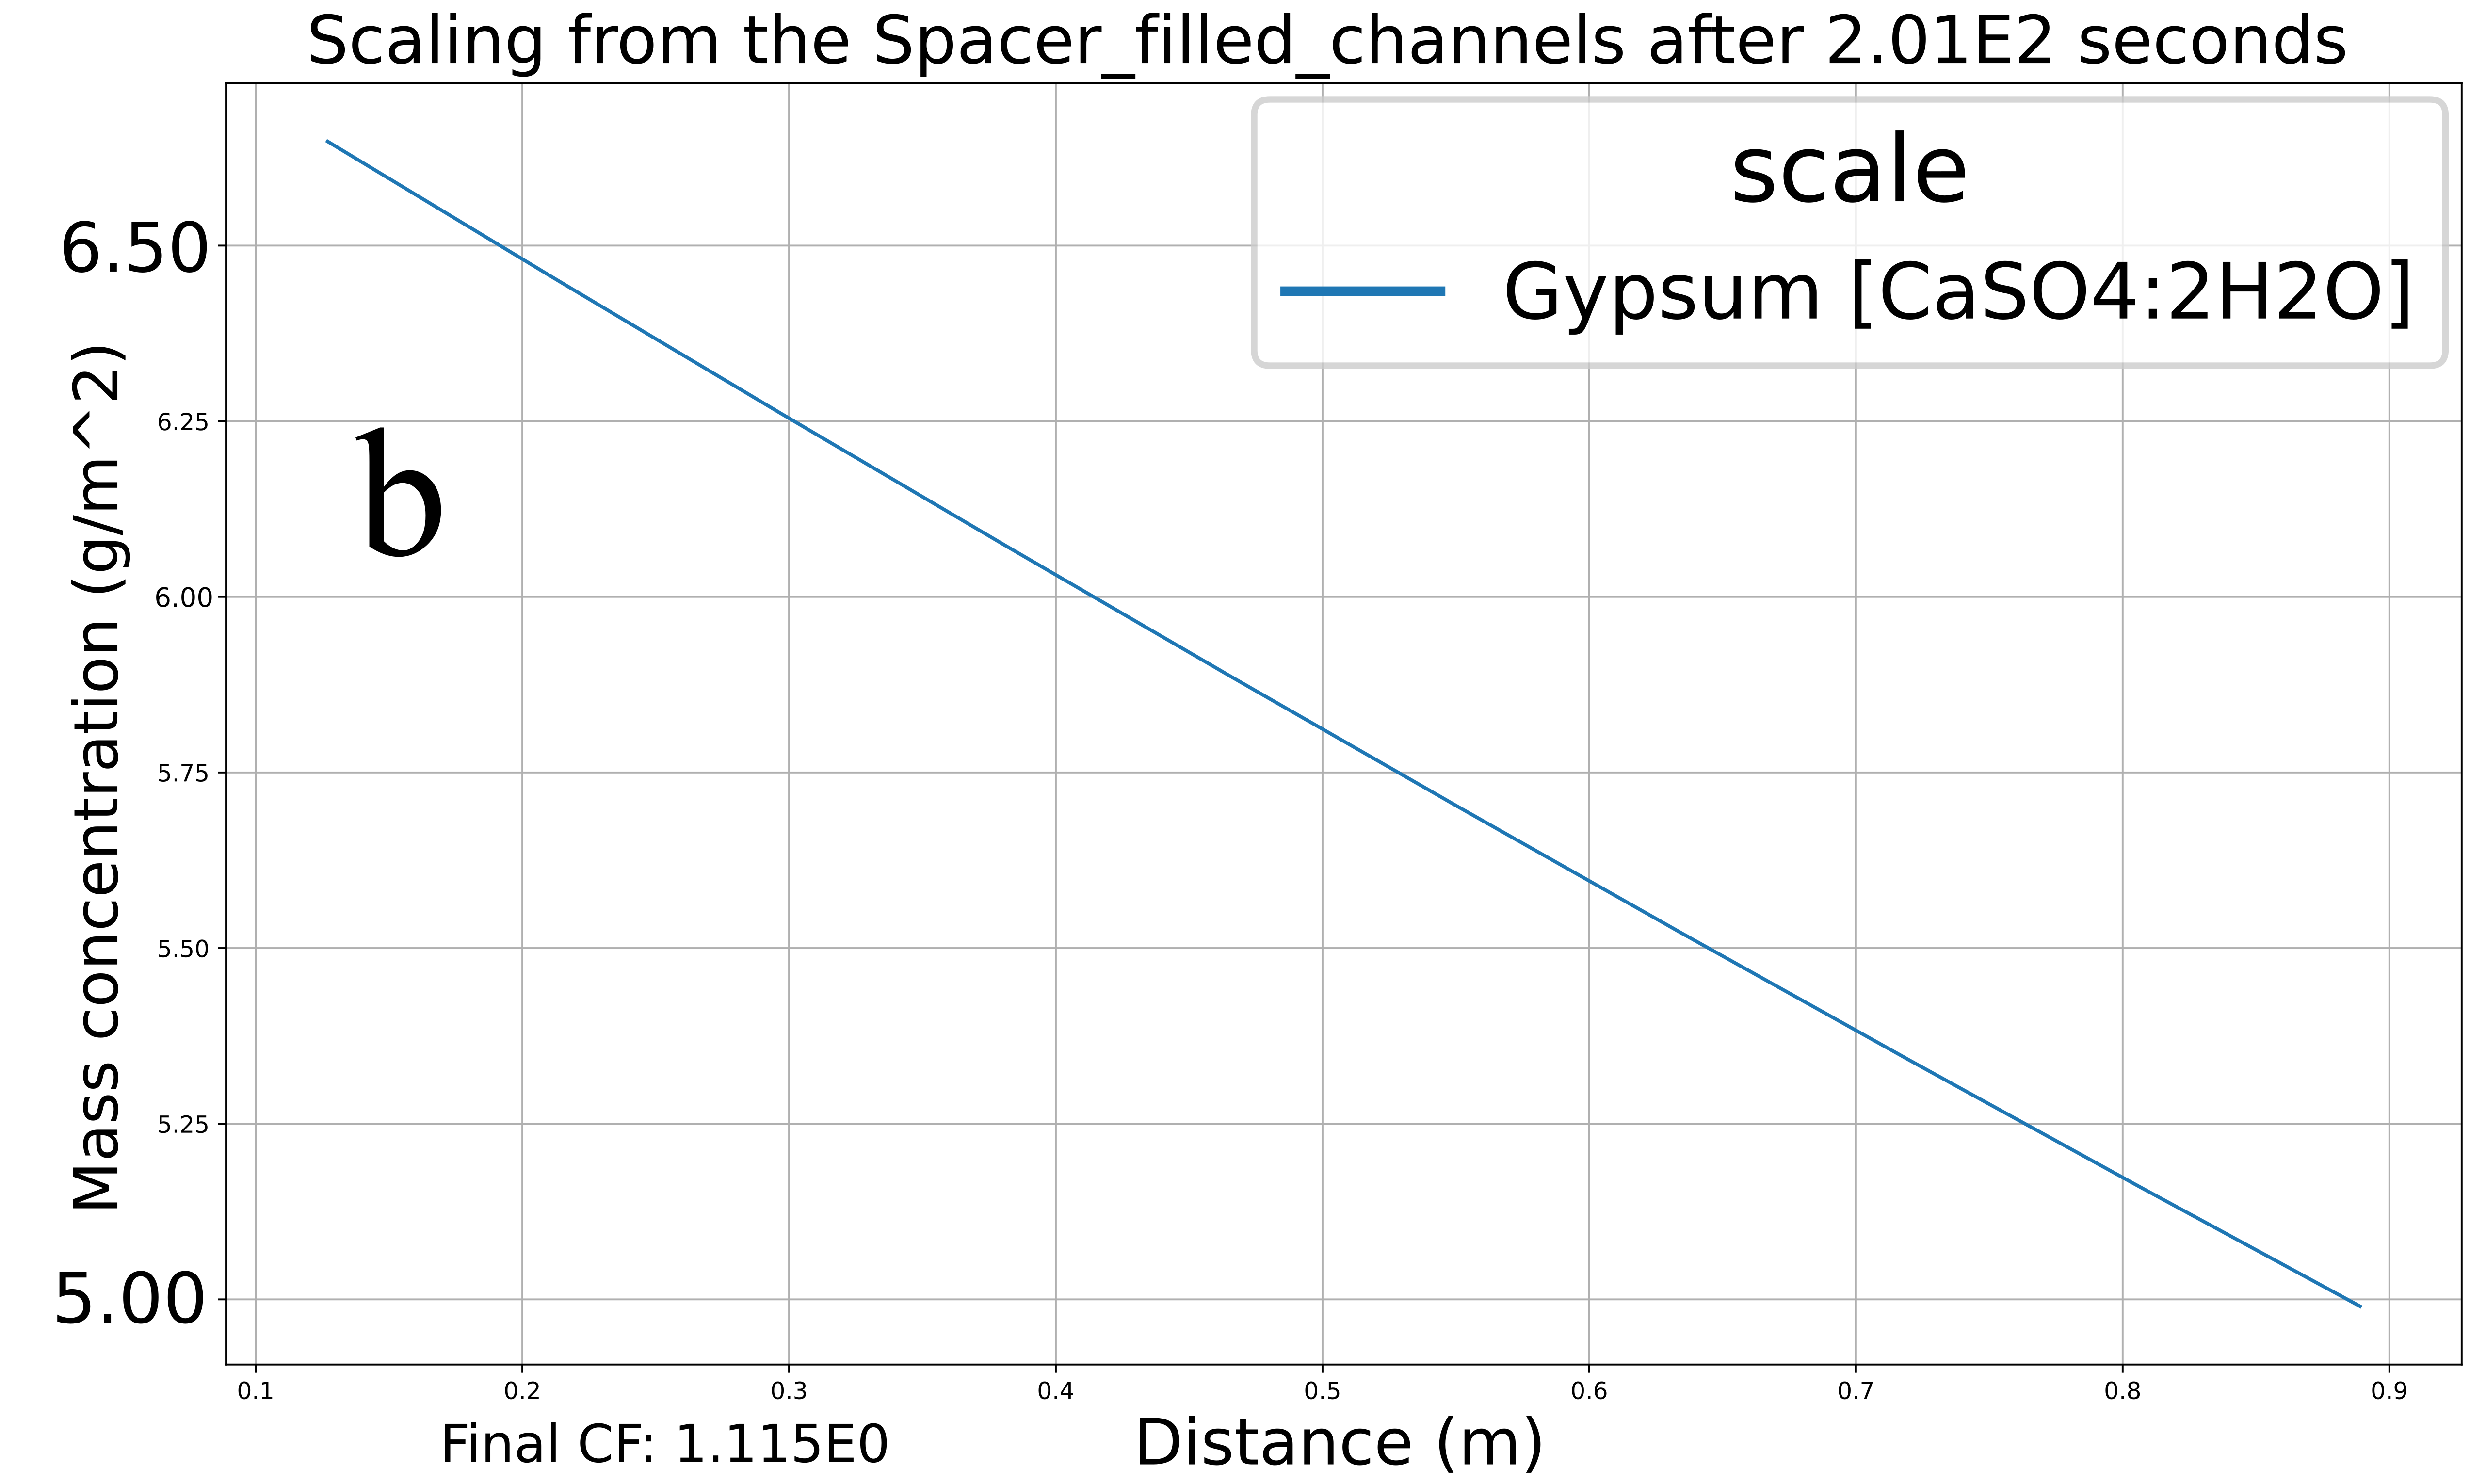
\includegraphics[width=0.49\linewidth]{images/ROSSpy/case_studies/Karabelas_2014_pitzer.png} 
        & 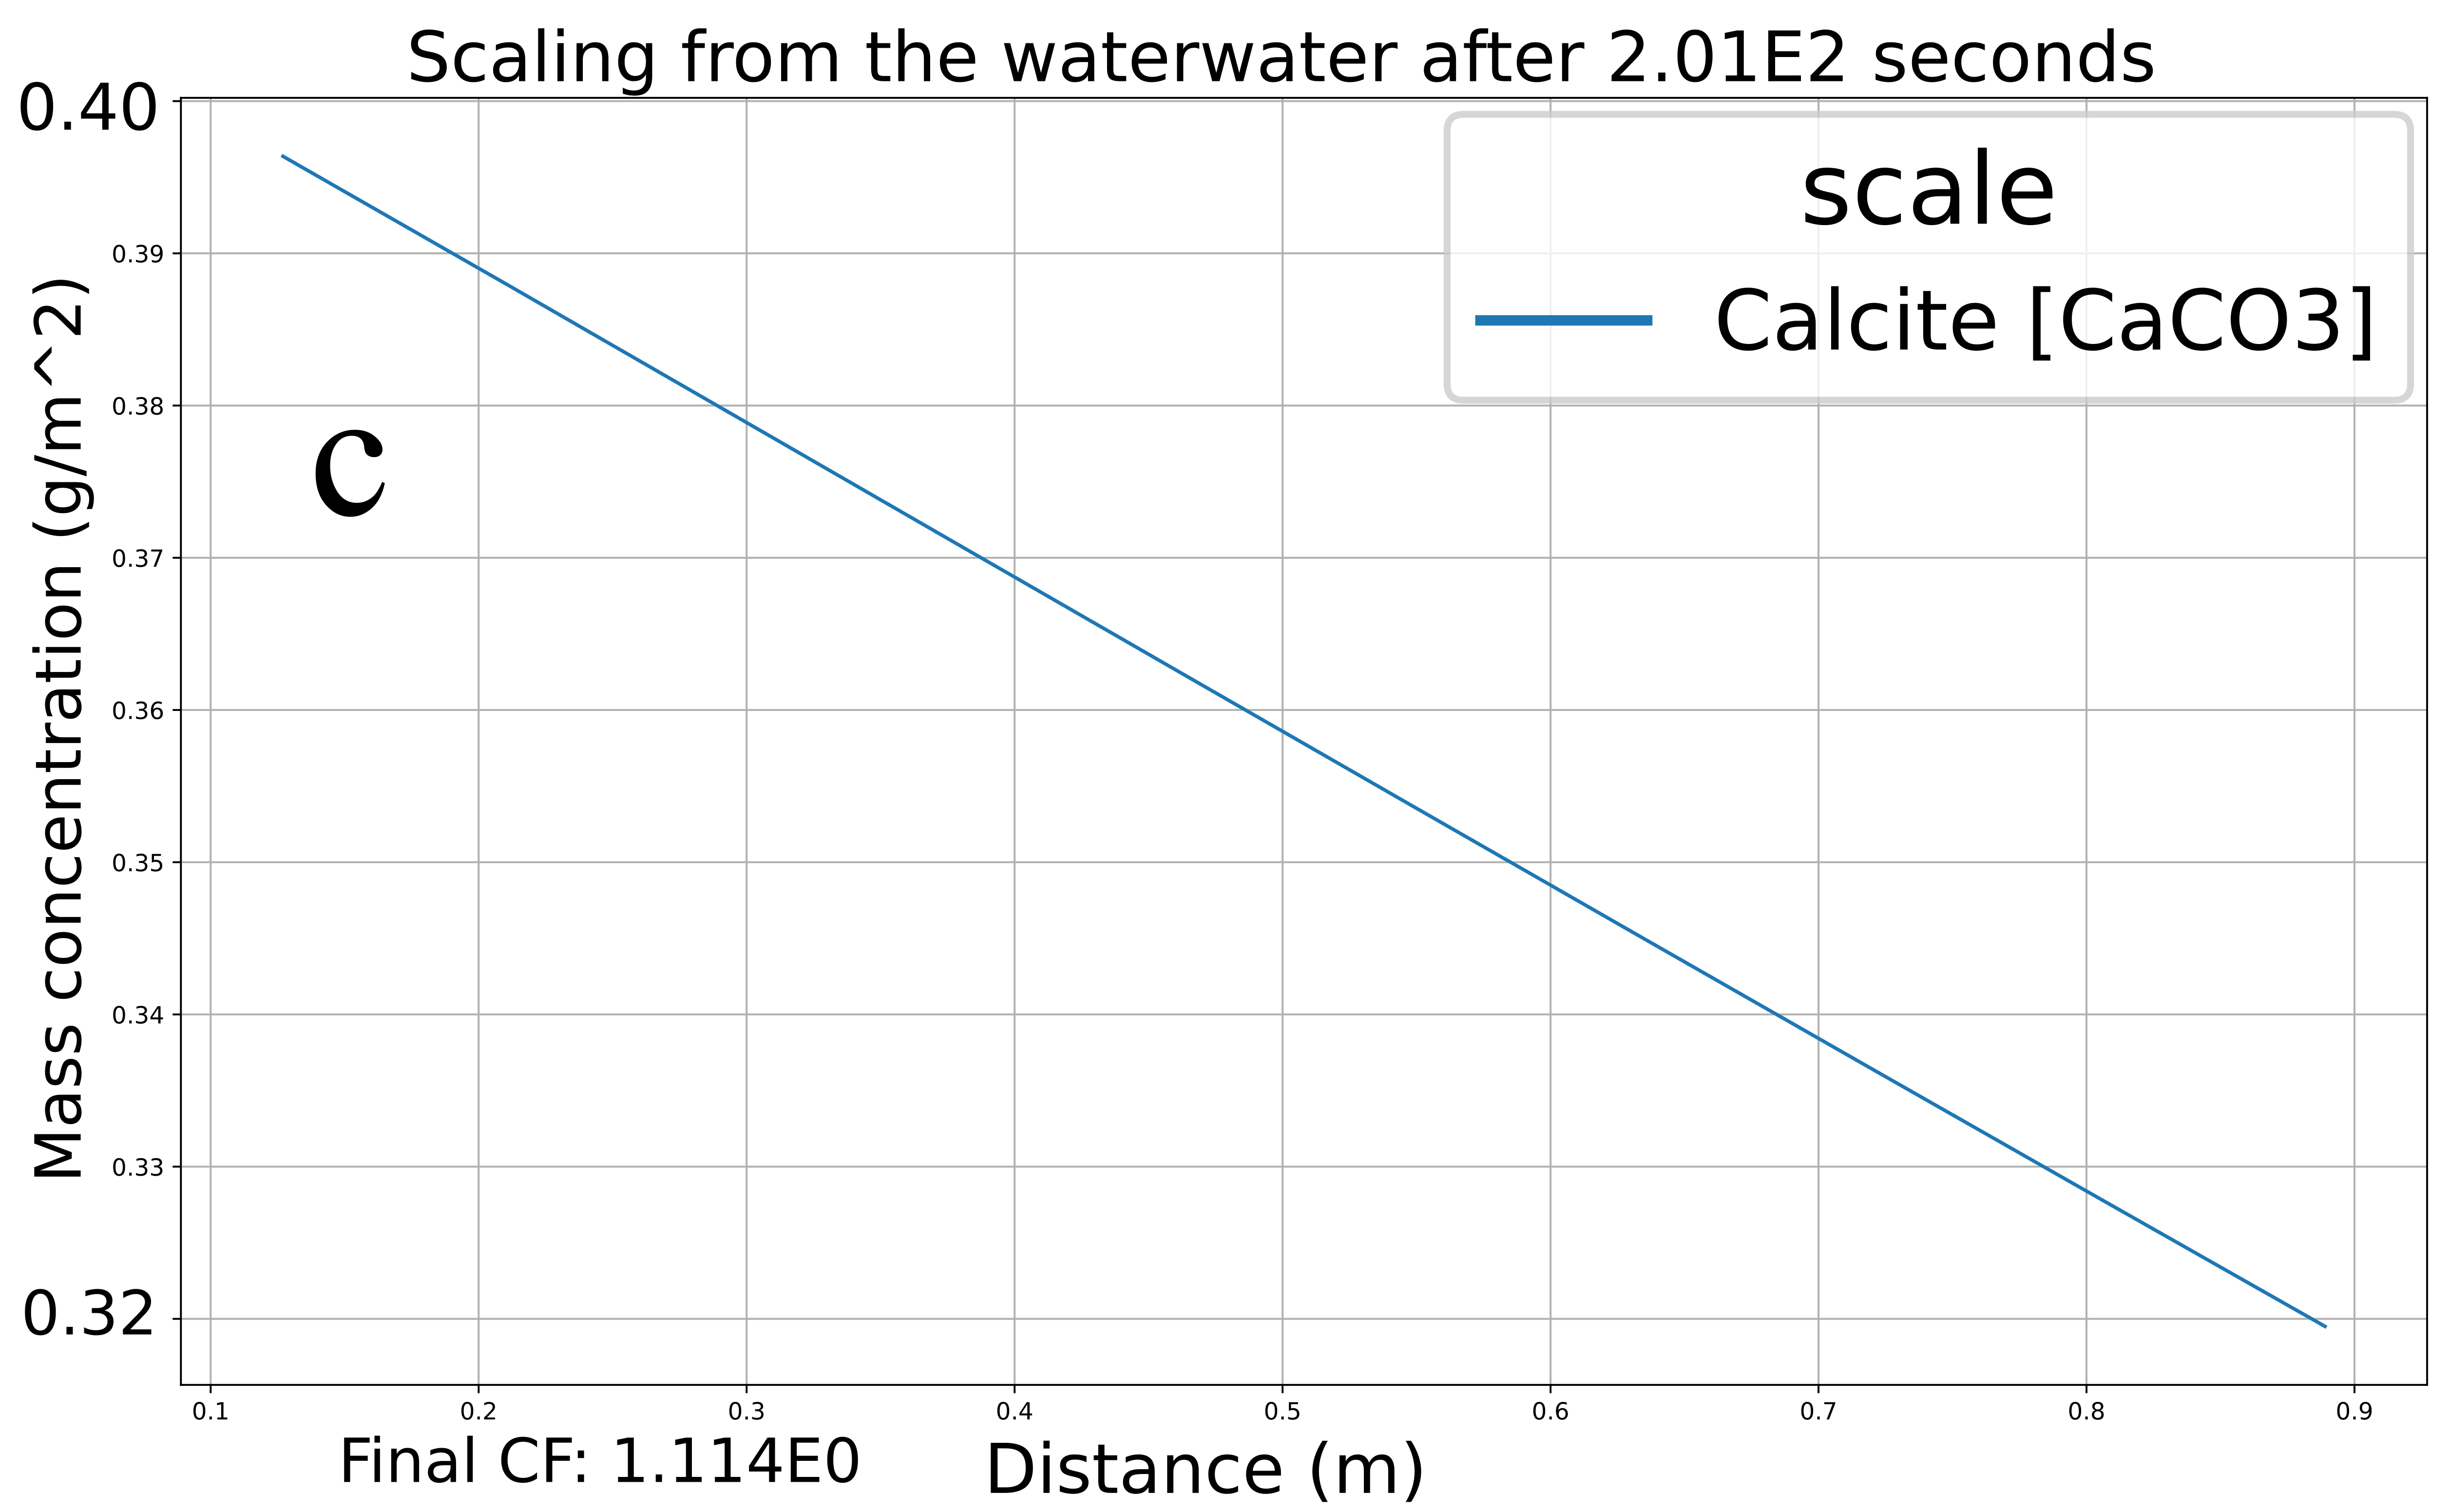
\includegraphics[width=0.49\linewidth]{images/ROSSpy/case_studies/Lee_pitzer.png} \\
    \end{tabular}
    \caption{
        The qualitative validation of scaling for a) multiple minerals from the Karabelas et al., 2020 study; for b) Gypsum in the Karabelas et al., 2014 study; or for c) Calcite in the Lee et al. study.
    }
    \label{qualitative_scaling}
\end{figure}


\section{Sensitivity analyses}
A few sensitivity analyses were conducted with major parameters in the following subsections. Additional sensitivity analyses of lesser parameters are presented in the Supporting Information.

\subsection{Database section}
The PHREEQC databases crucially define the geochemistry of each simulation. The database selection 1) determines the set of minerals that can be simulated; 2) contains all of the kinetic, thermodynamic, and stoichiometry information of each mineral; and 3) applies a chemical model -- e.g. Pitzer, Debye-H\"uckel, and Davies in Section 7 of the Supporting Information -- to calculate the precipitation equilibria of scaling. The database therefore quantitatively and qualitatively influences the scaling predictions from ROSSpy. The Pitzer model \cite{Pitzer1973ThermodynamicsEquations,Pitzer1974ThermodynamicsElectrolytes} is touted as being supremely accurate in the concentration range that is common for desalination \cite{VandeLisdonk2001PredictionSystems,Sheikholeslami2004AssessmentUnits,Mohammad2007PredictionMembranes}. The Pitzer PHREEQC database is therefore the default option for ROSSpy, however, the narrow range of ions and minerals that are accepted by the Pitzer model may justify using databases, such as wateq4, for complex feed sources with a large variety of ions.

A standard set of simulation conditions and feed water from the Red Sea was conducted with each PHREEQC database. These conditions failed to numerically converge for $\frac{4}{13}$ of the databases -- $Amm$, $Core10$, $LLNL$, and $Minteq.v4$. The results of the other $\frac{9}{13}$ databases are summarized in Figure \ref{database_selection}, where the selection of PHREEQC database -- and thus the chemical model and database contents -- significantly changes scaling predictions. The database should therefore be selected after review of the PHREEQC User Manual or by inquiry to the PHREEQC user forum \url{PHREEQCusers.org} to make the proper selection for the simulated system.

\begin{figure}[h]
    \centering
    \begin{tabular}{c|c}
        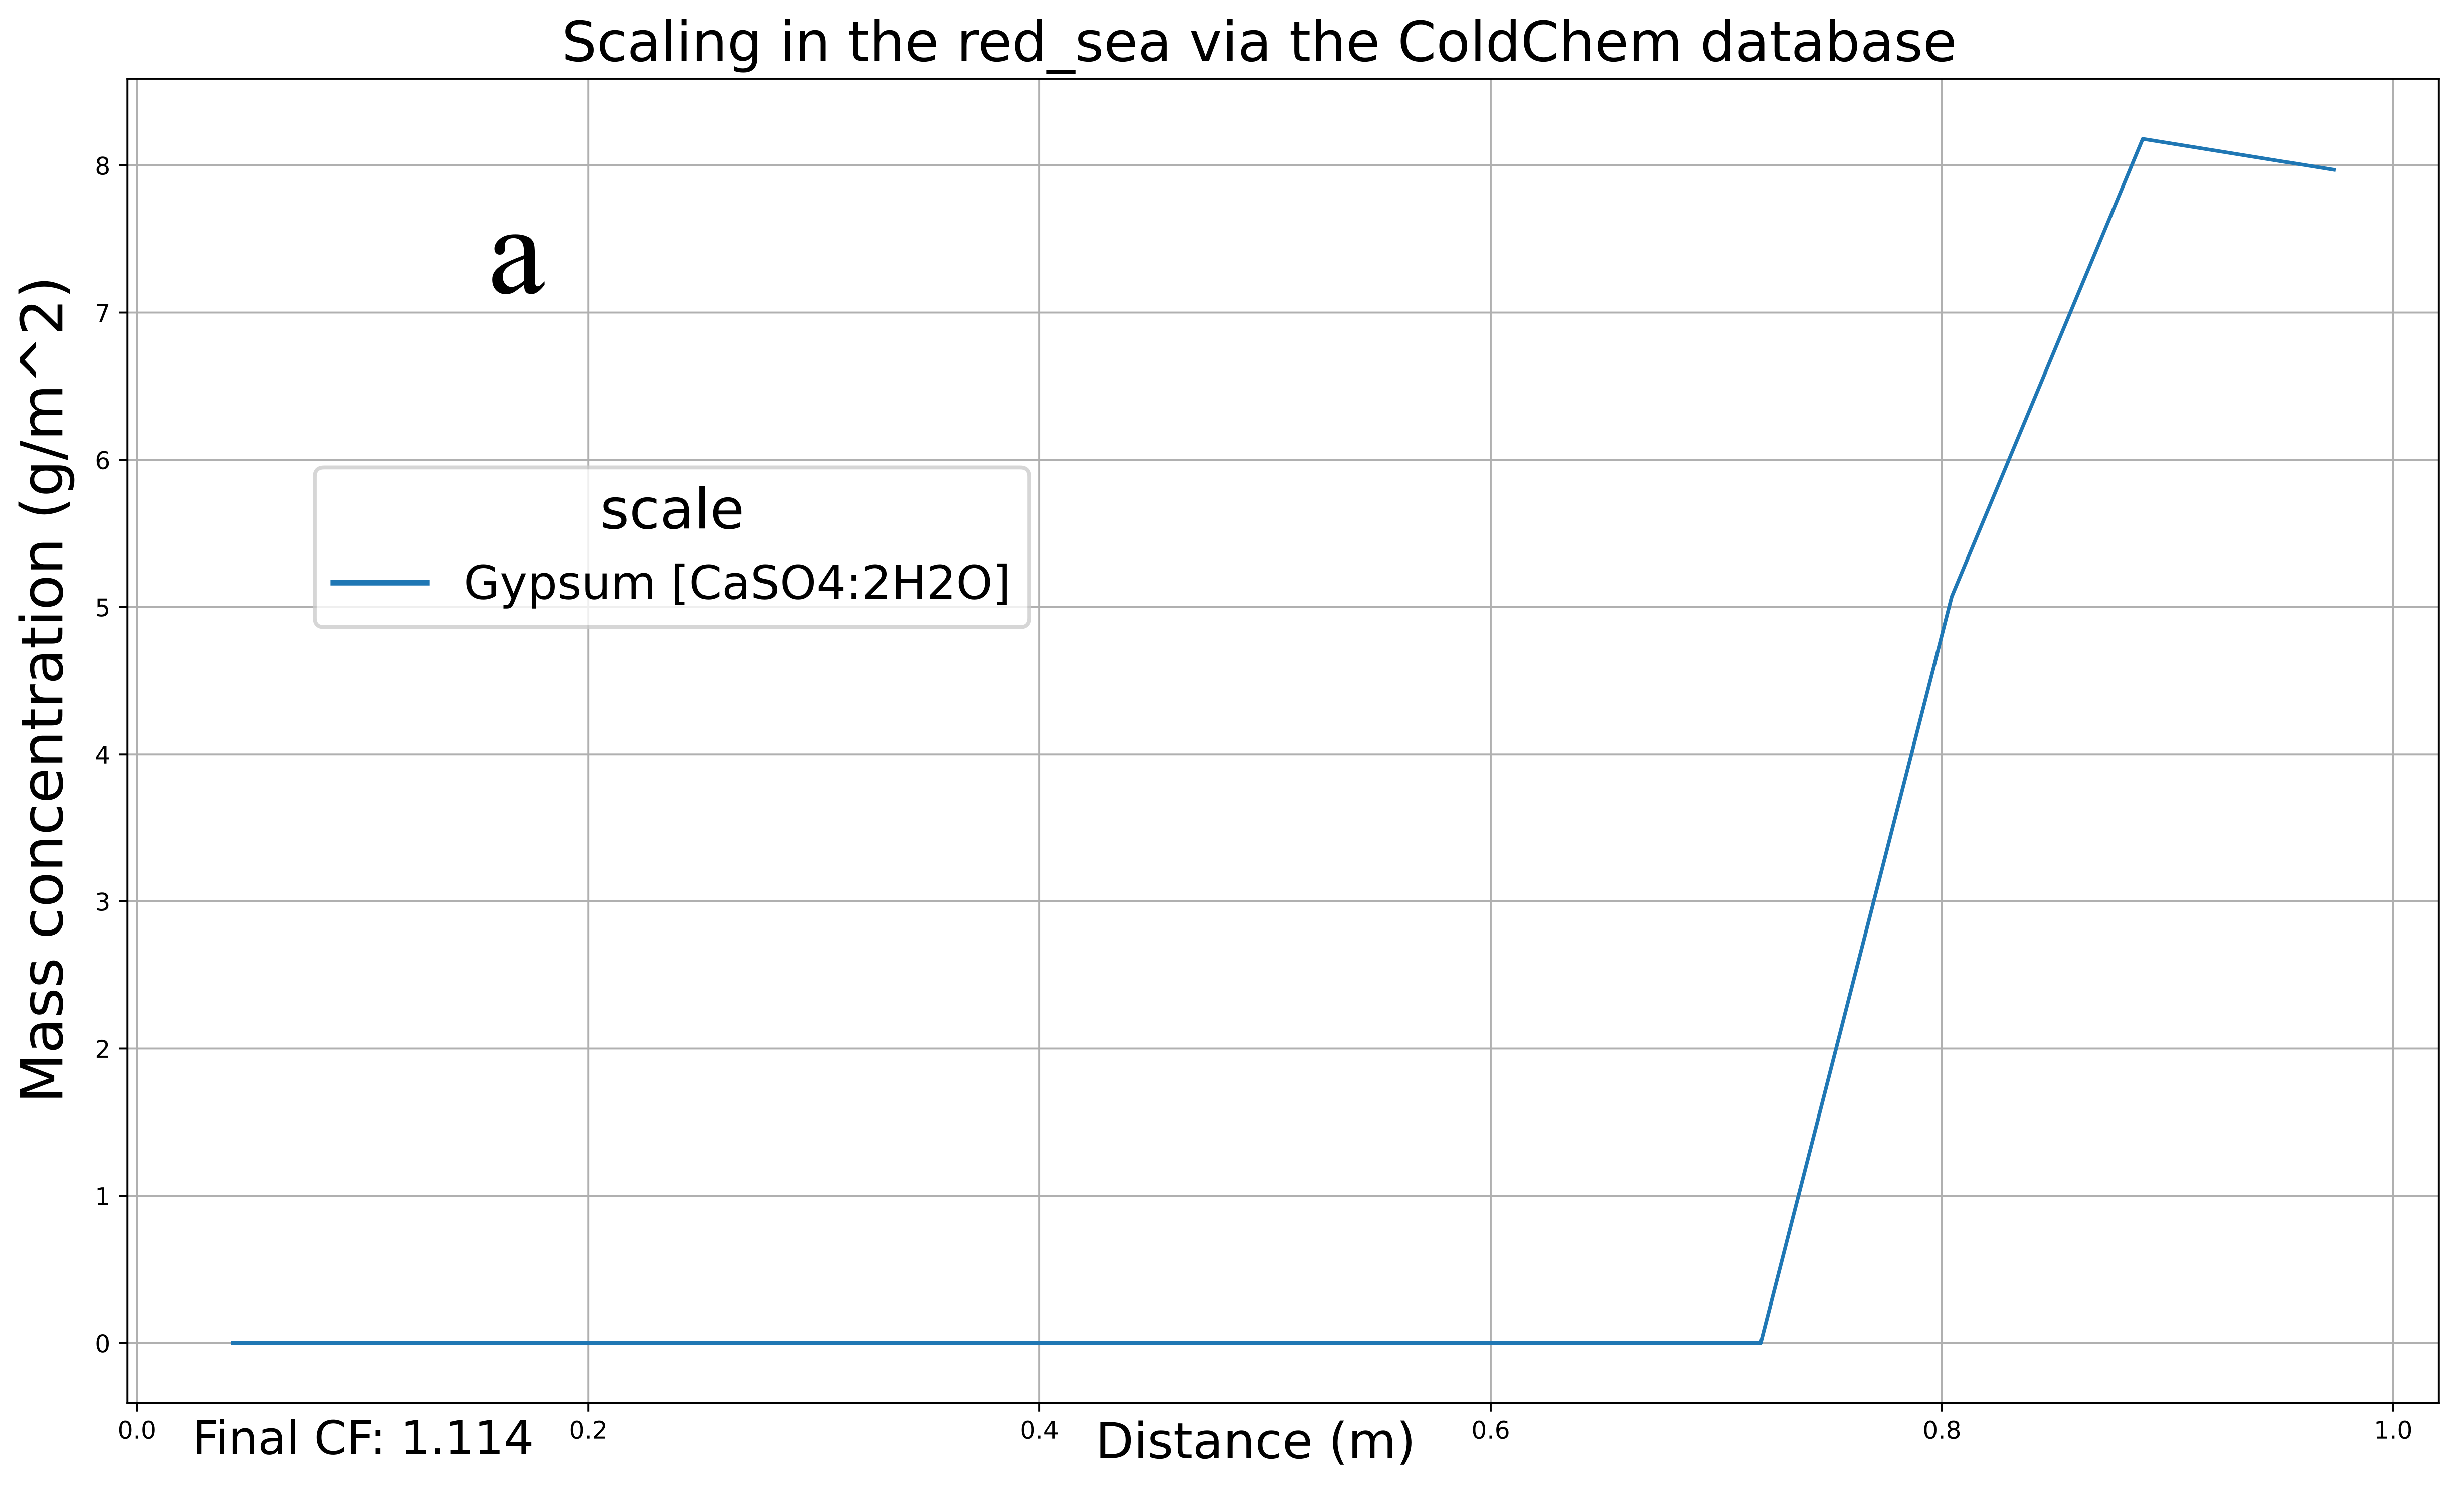
\includegraphics[width=0.49\textwidth]{images/ROSSpy/sensitivity_analyses/databases/ColdChem.png} 
        & 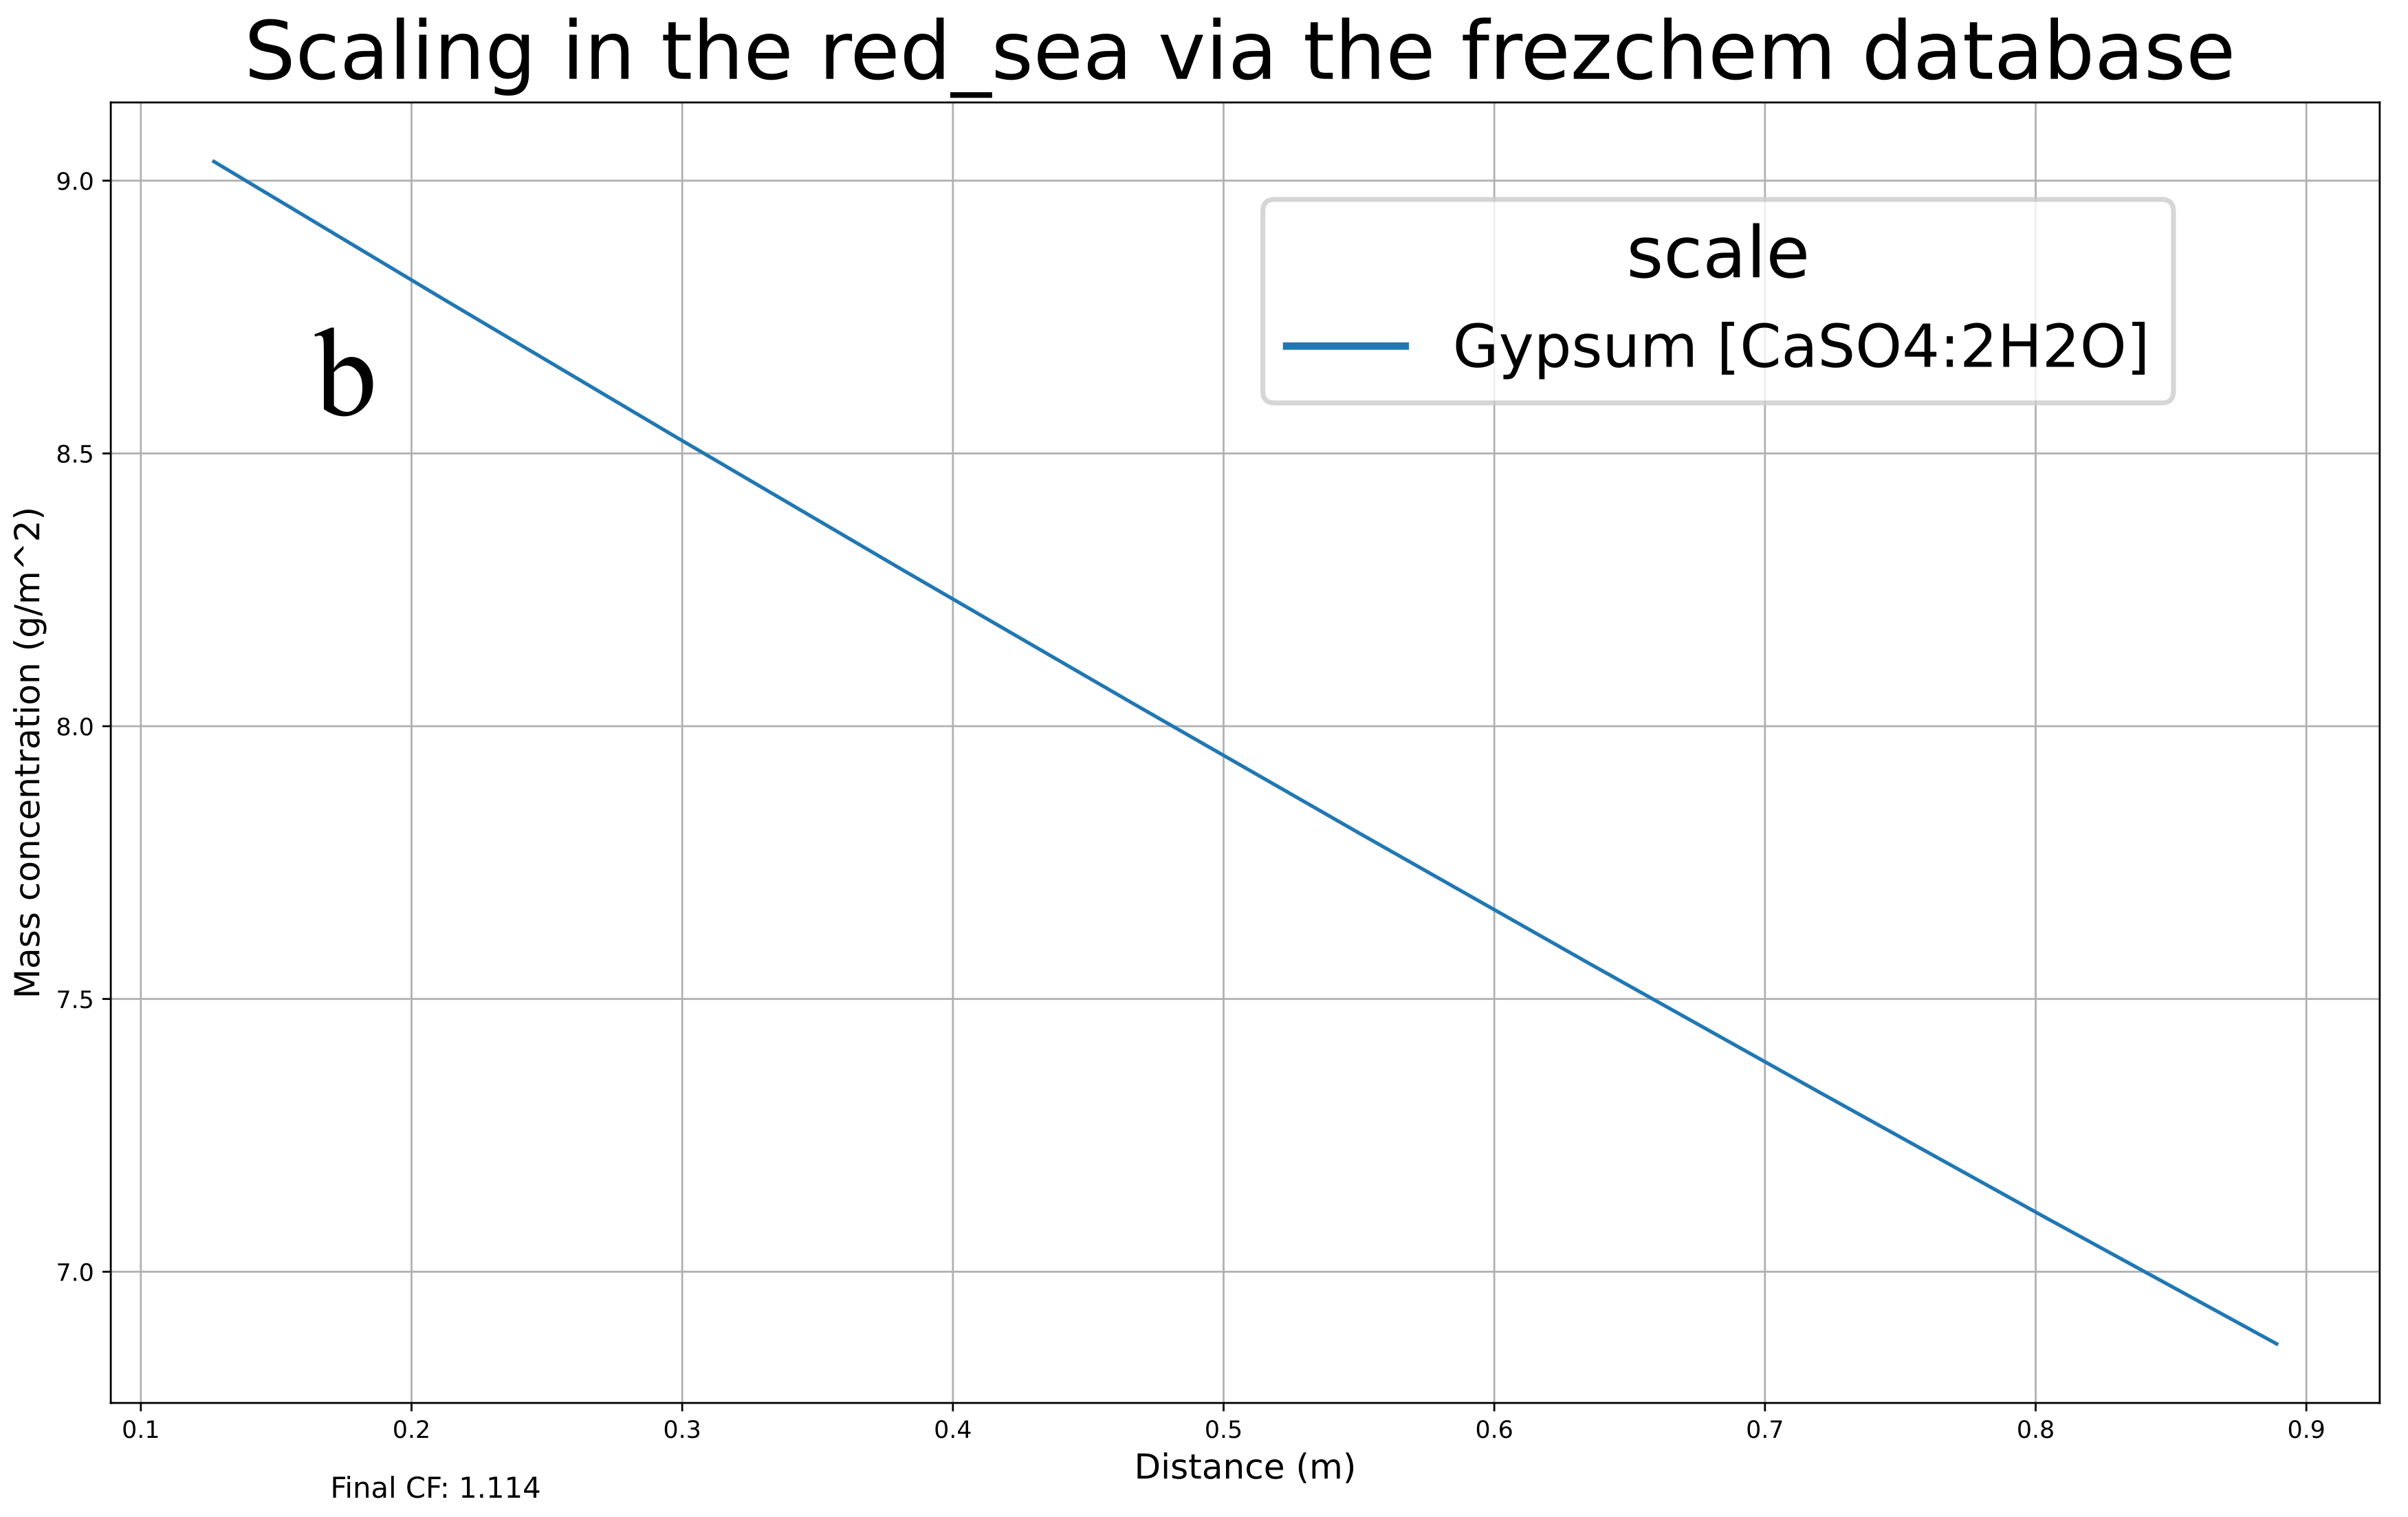
\includegraphics[width=0.49\textwidth]{images/ROSSpy/sensitivity_analyses/databases/FreezChem.png} \\ \midrule 
        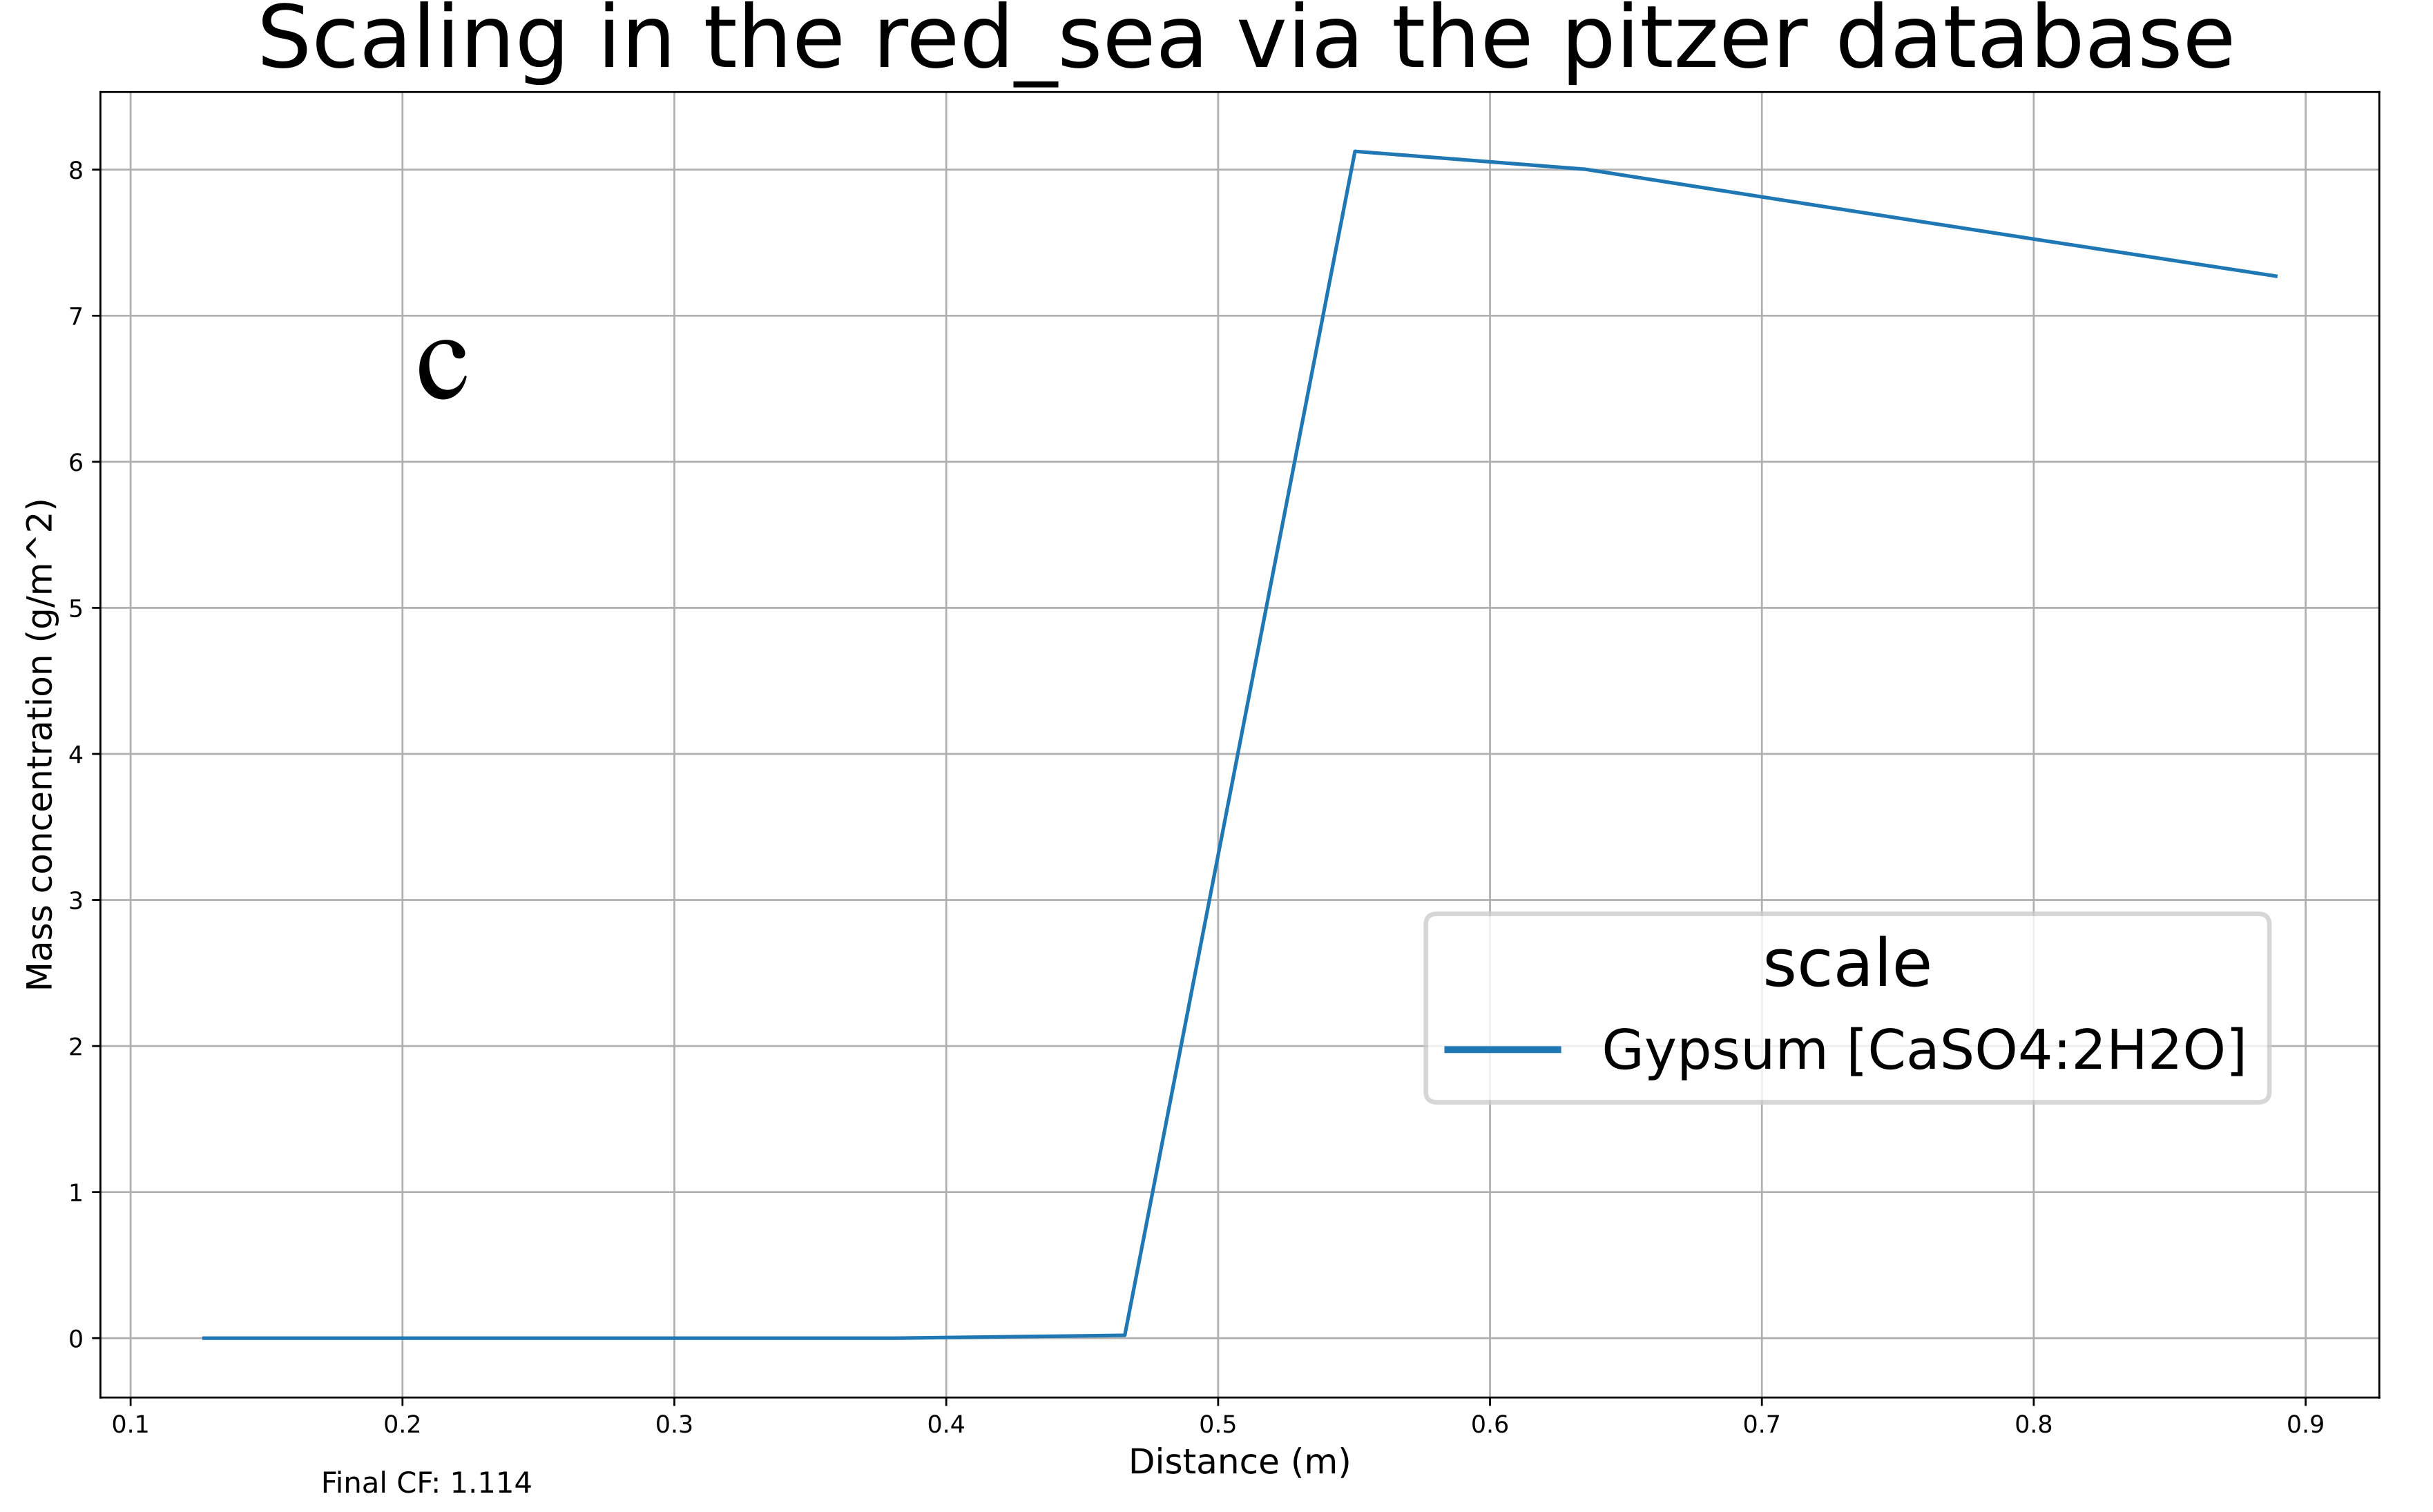
\includegraphics[width=0.49\textwidth]{images/ROSSpy/sensitivity_analyses/databases/Pitzer.png} 
        & 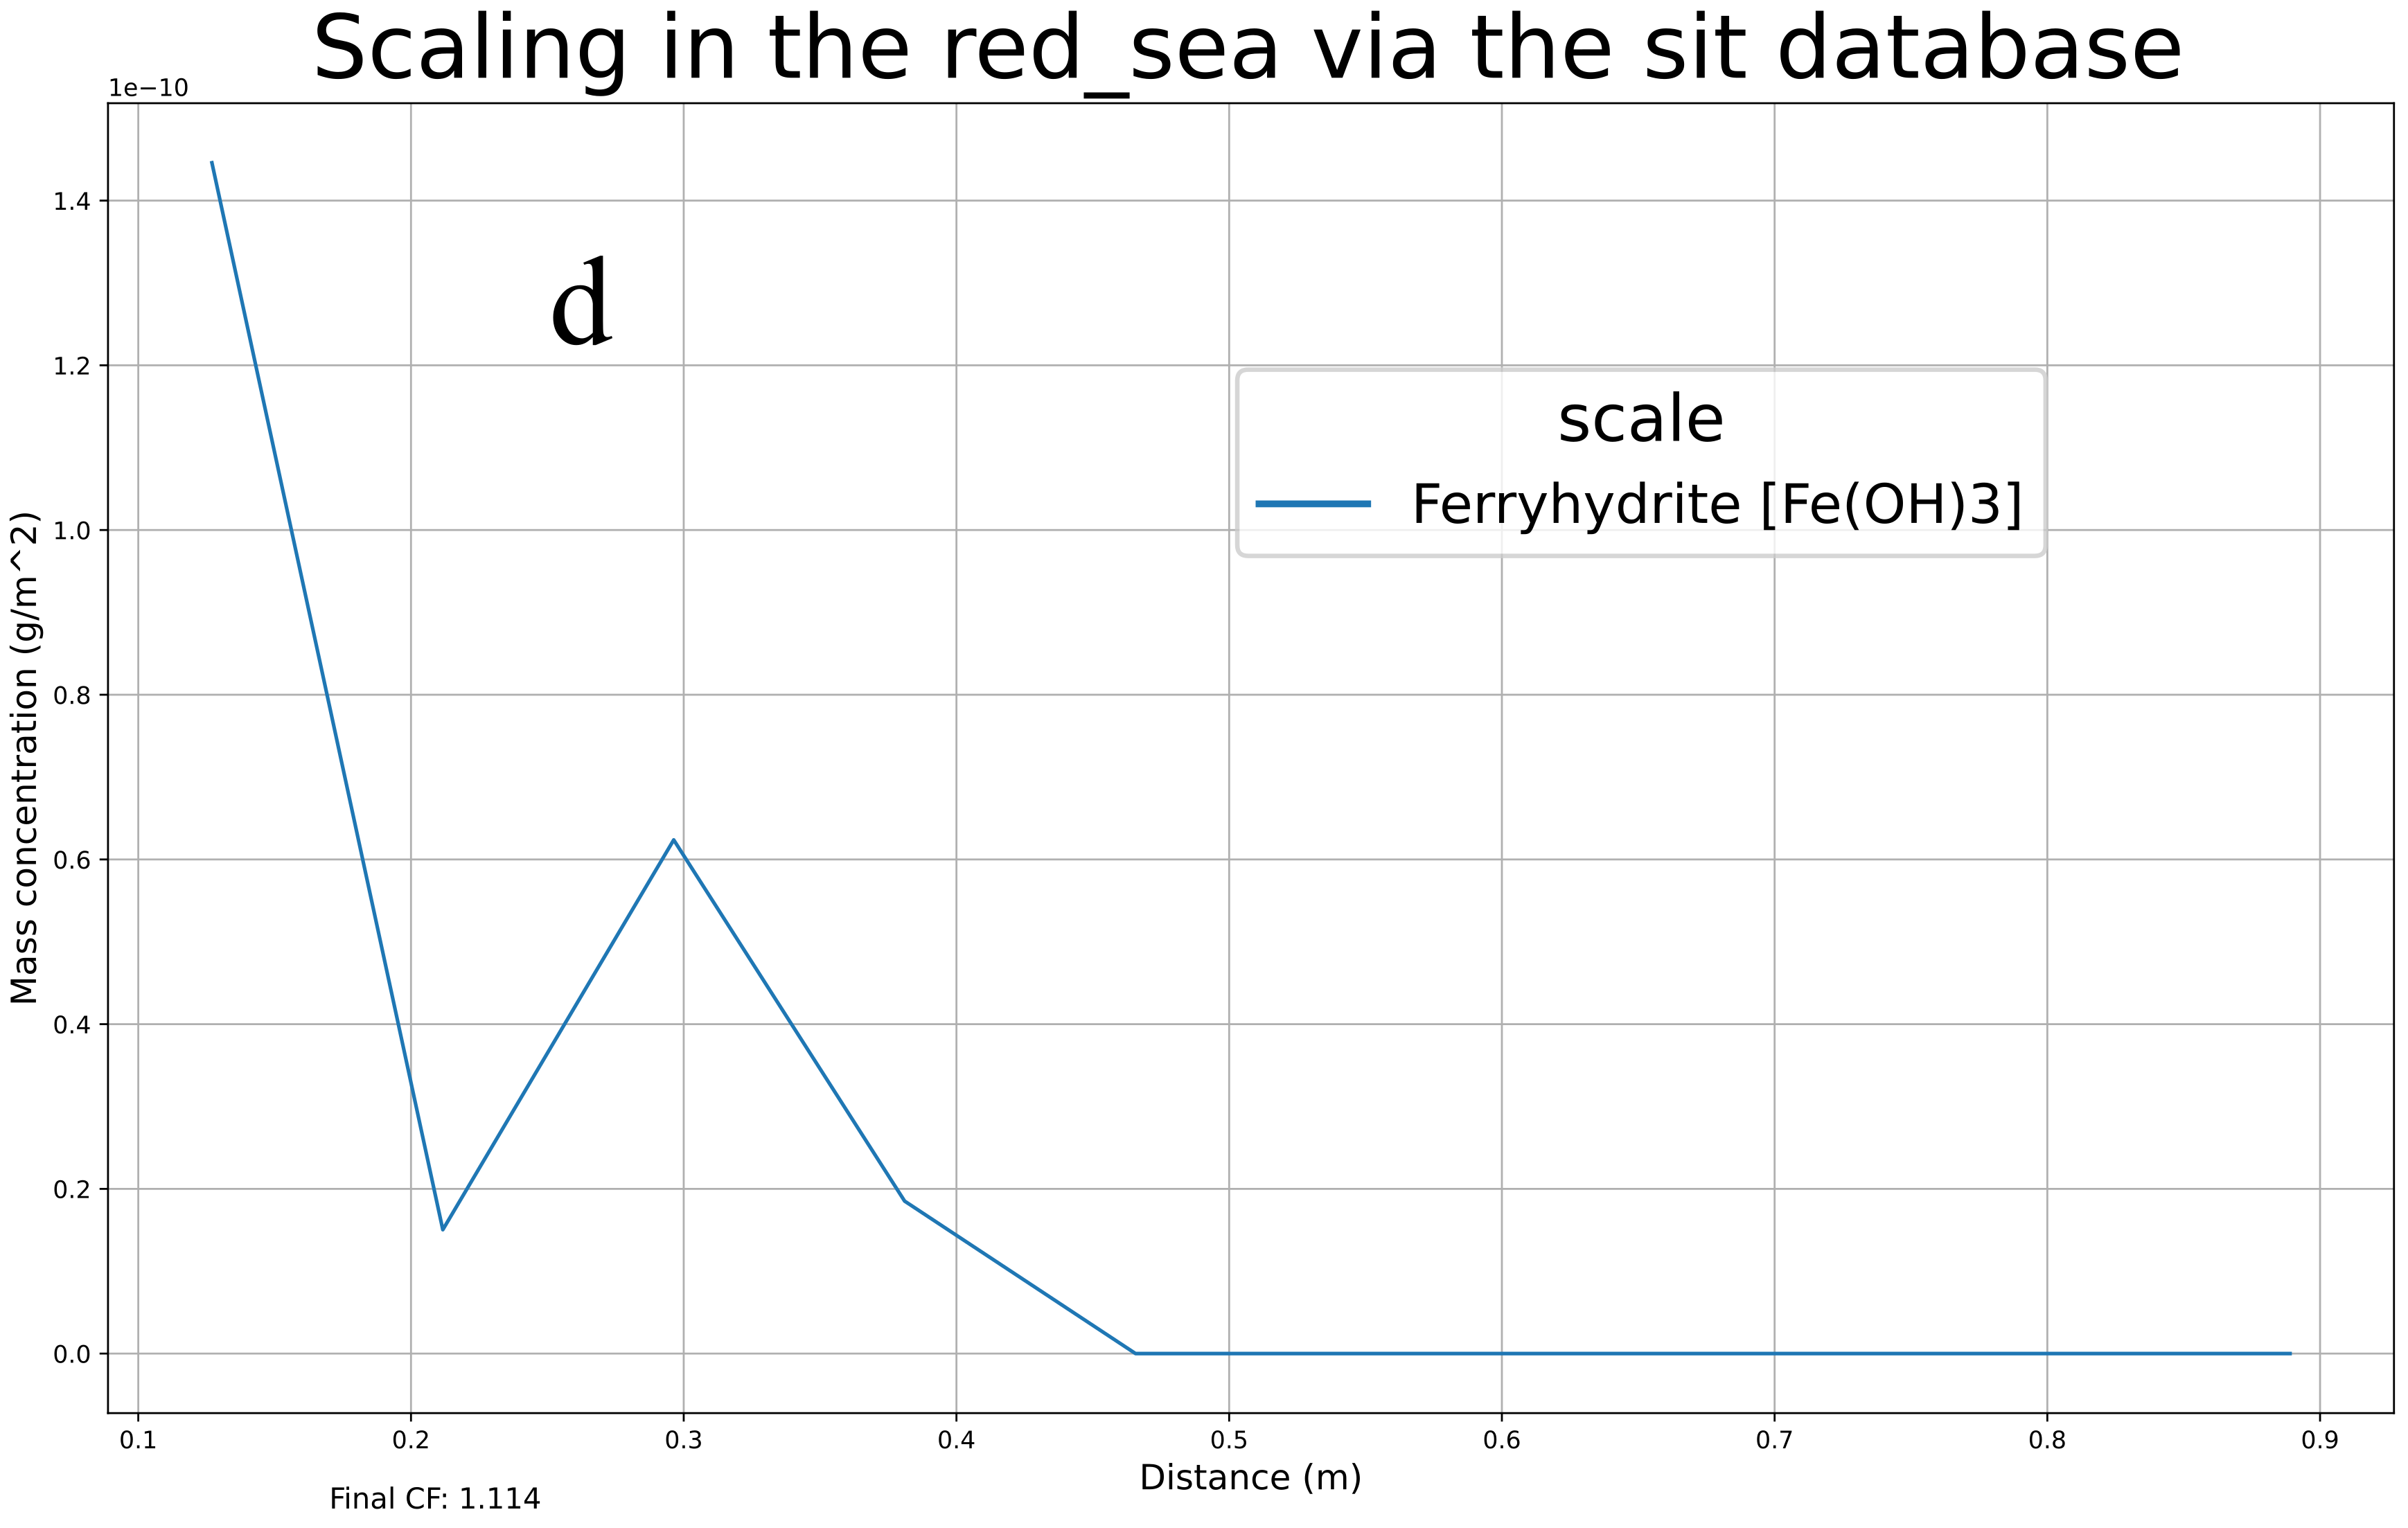
\includegraphics[width=0.49\textwidth]{images/ROSSpy/sensitivity_analyses/databases/Sit.png} 
        \\ \bottomrule
    \end{tabular}
    \caption{
        Scaling predictions from the a) ColdChem, b) FreezChem, c) Pitzer, and d) Sit databases, with otherwise identical simulation parameters.
    }
    \label{database_selection}
\end{figure}

\subsection{Simulation perspective}
Two simulation perspectives -- either 1) the entire module at the final time, primarily for scaling figures \cite{Chai2007UltrasoundModules}, or 2) all of the time at the module end, primarily for brine figures -- can be visualized through ROSSpy. These perspectives allow the multi-dimensional raw data to be sliced into one-dimensional sets that can be plotted against scaling density or brine concentrations: e.g. Figures \ref{brine_perspectives}-\ref{scaling_perspectives}. The raw data can alternatively be processed by the user through custom means after the data are exported from ROSSpy.

\begin{figure}[t]
    \centering
    \begin{tabular}{c}
        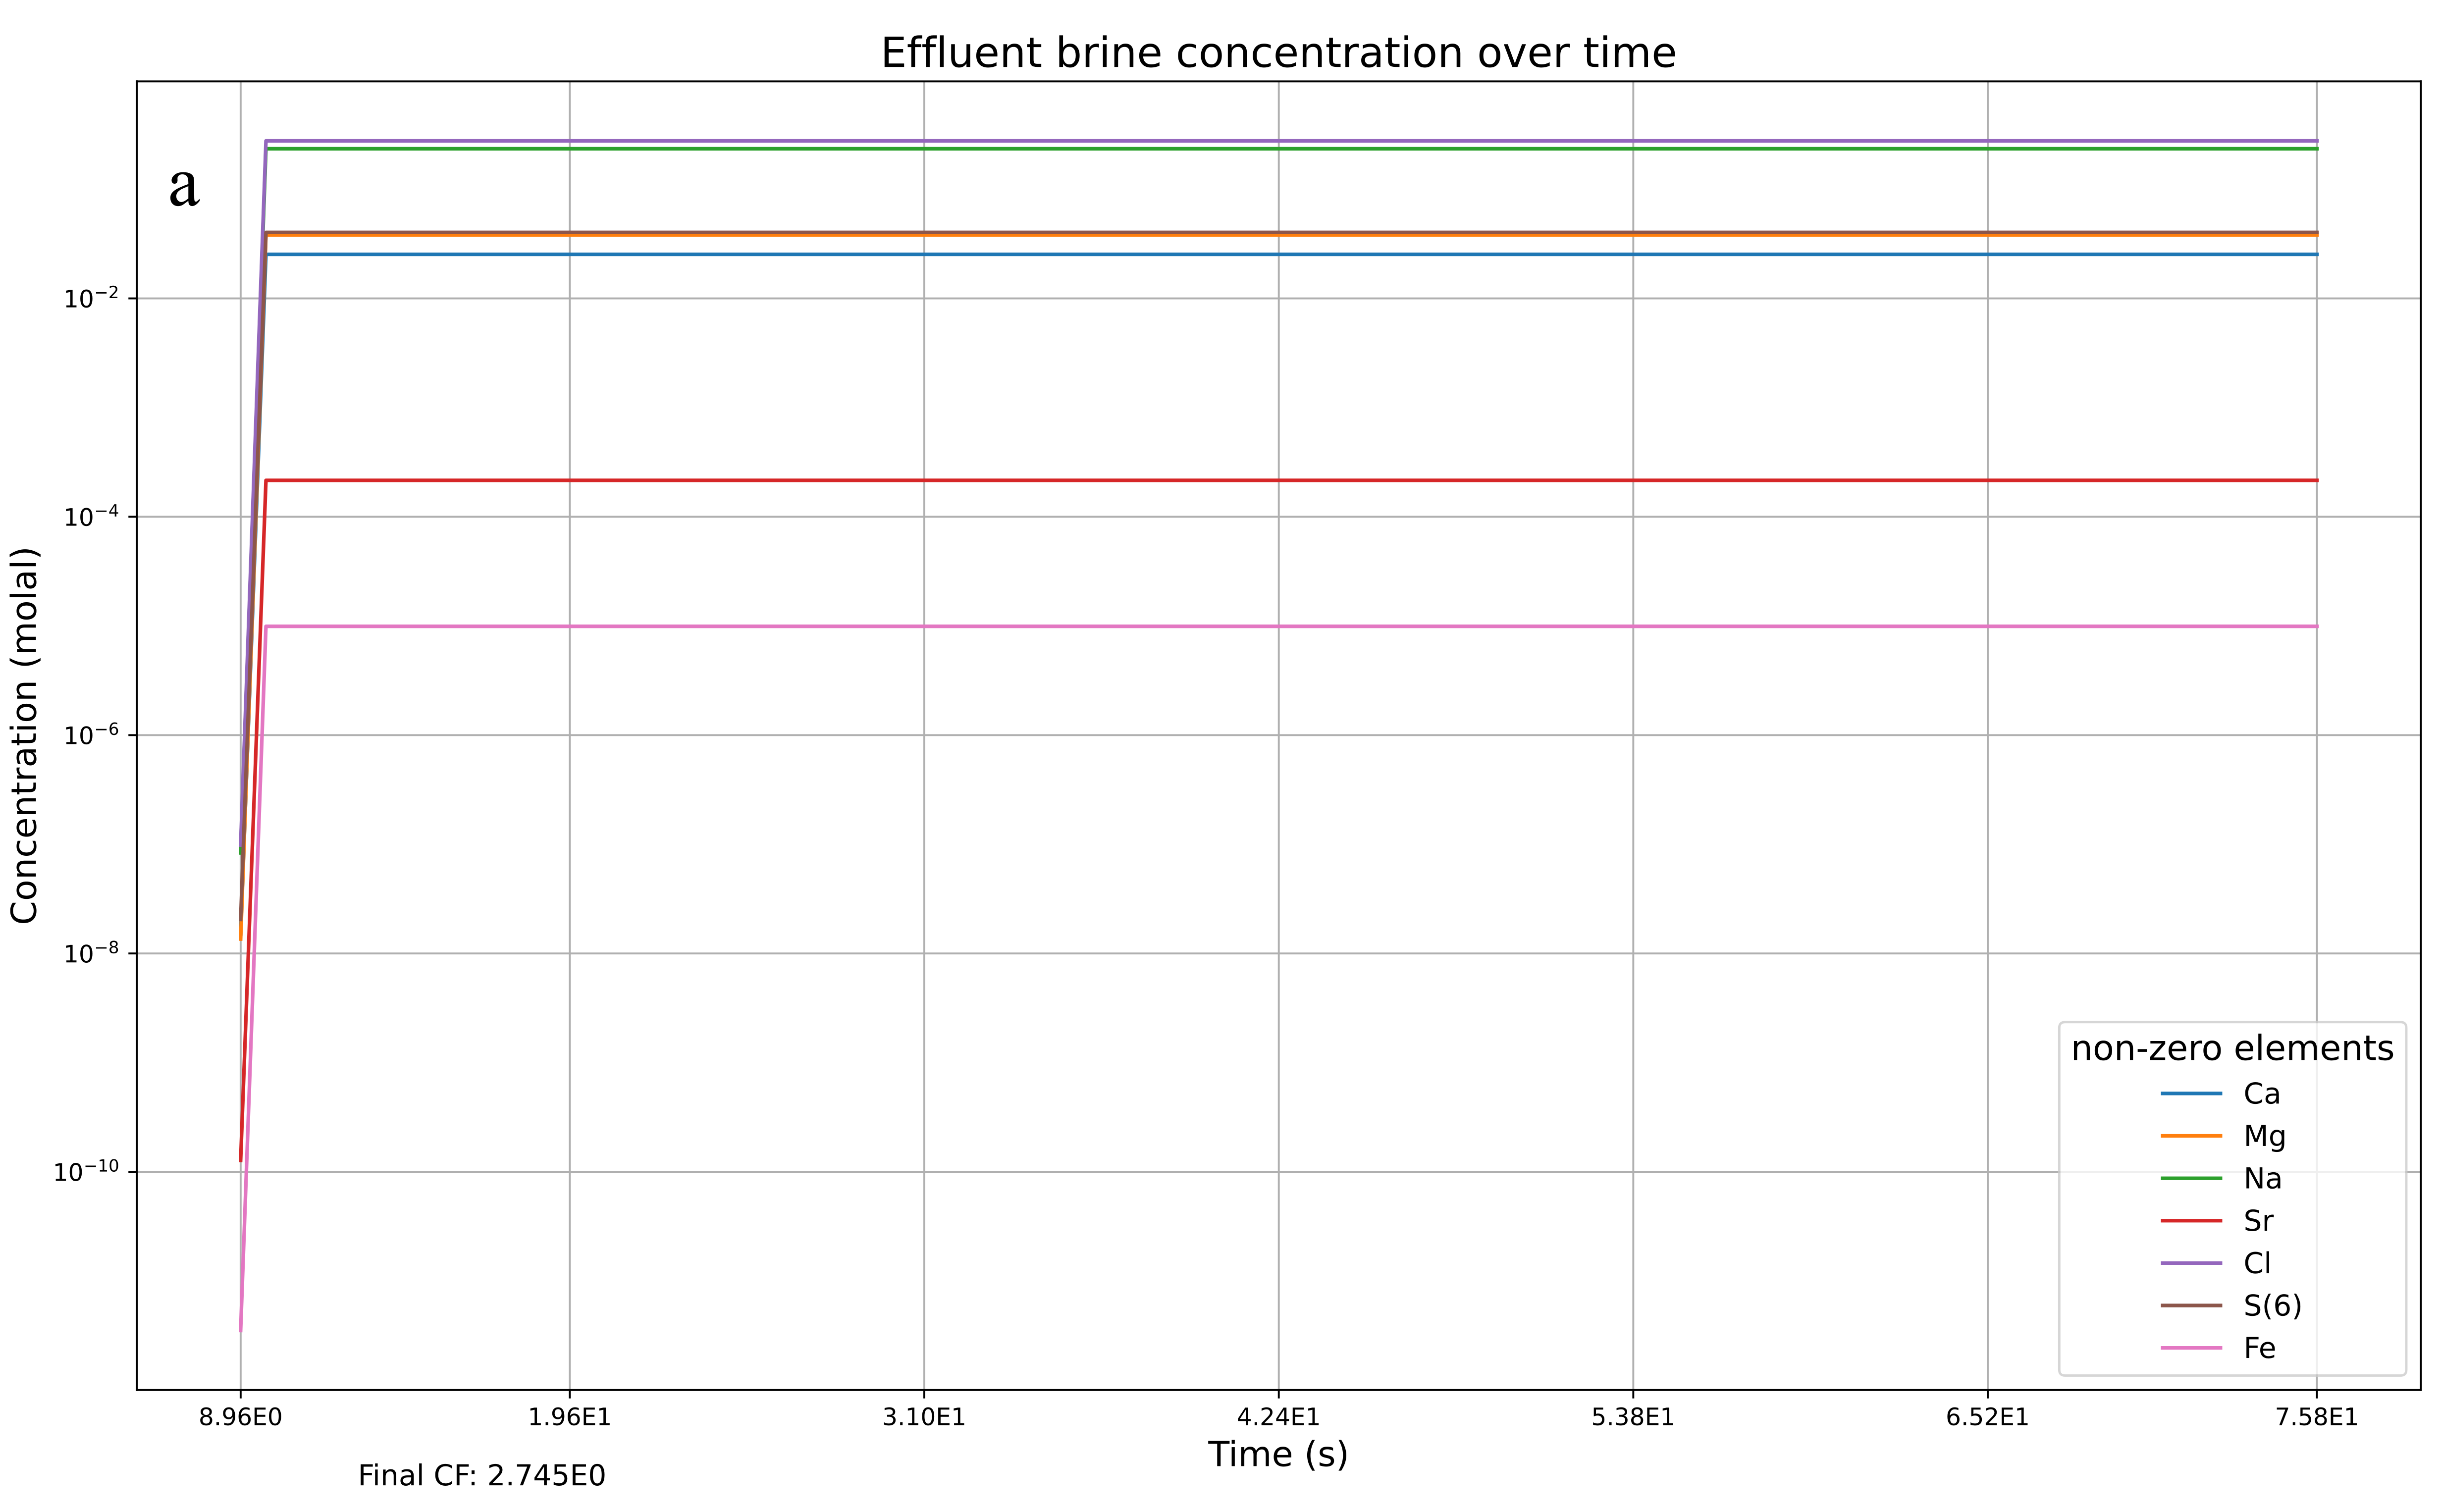
\includegraphics[width=\linewidth]{images/ROSSpy/sensitivity_analyses/simulation_perspective/brine_all_time.png} \\ \midrule
        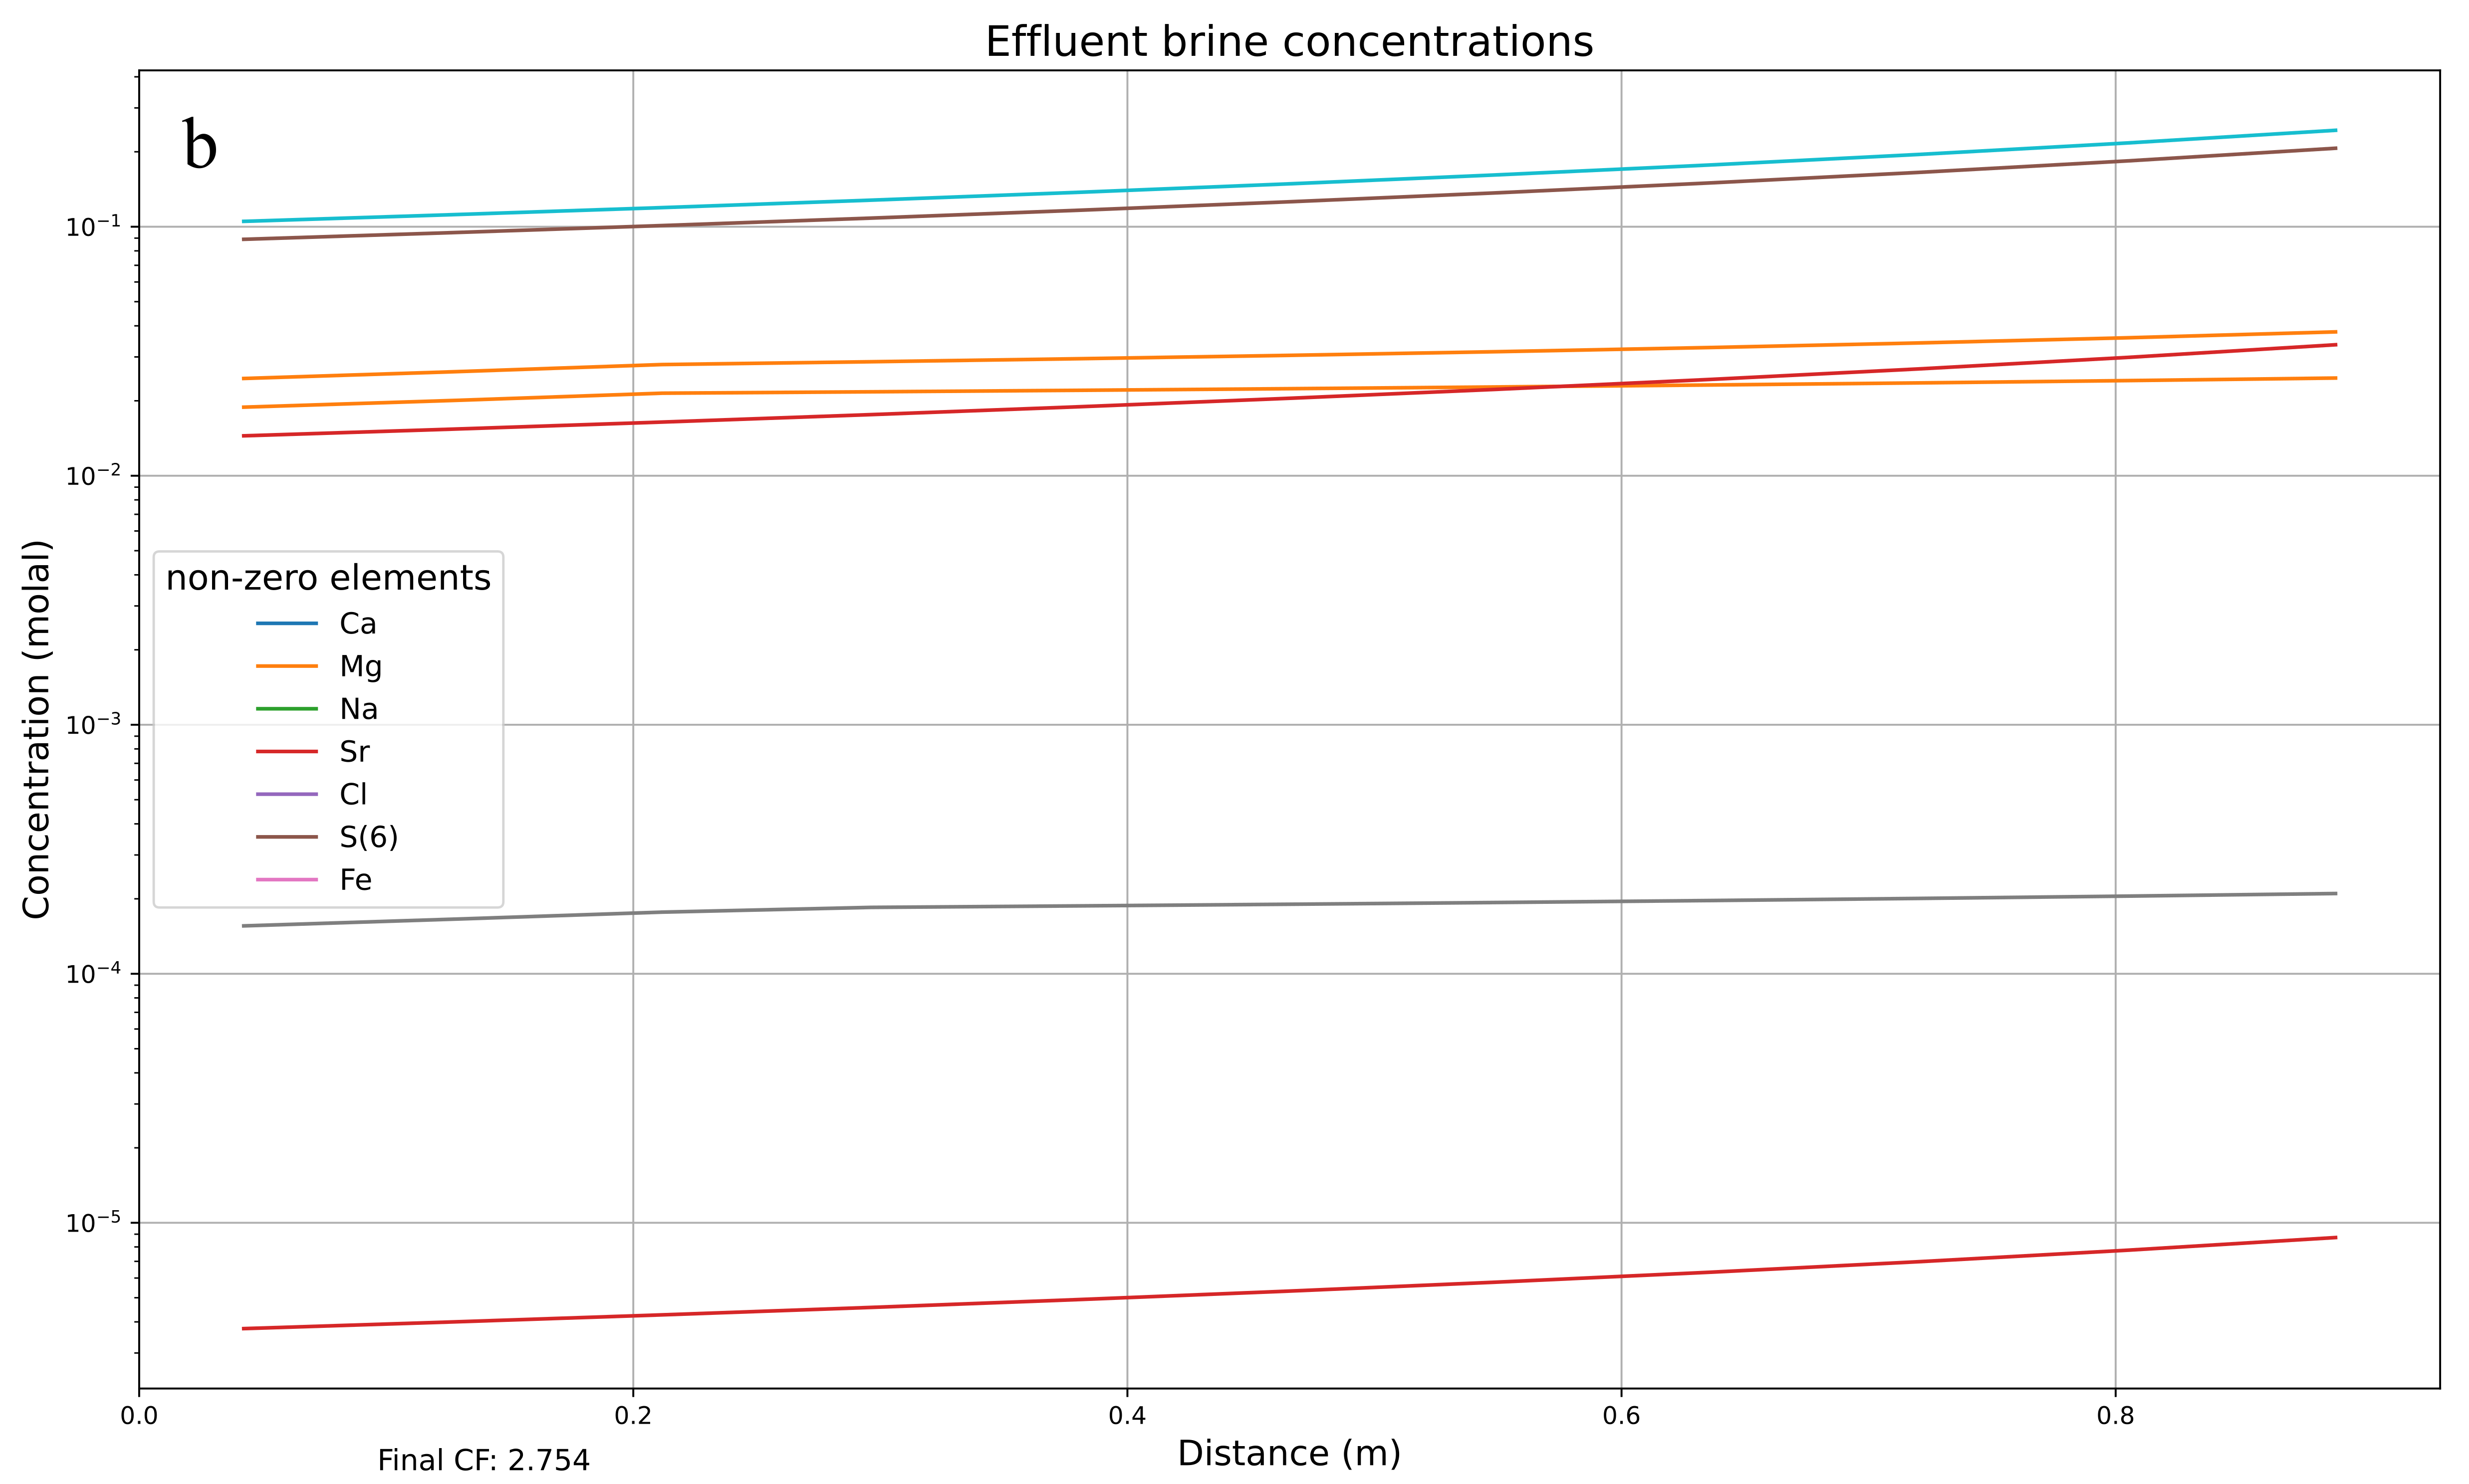
\includegraphics[width=\linewidth]{images/ROSSpy/sensitivity_analyses/simulation_perspective/brine_all_distance.png}
    \end{tabular}
    \caption{
        Brine formation while either a) slicing through time at the end distance or b) slicing  through distance at the final time. The final concentrations differ slightly between the two simulation perspectives, where the all\_time perspective calculates the true end of the last cell while the all\_distance perspective calculates the mid-point of the last cell and thus has a slightly lower concentration. 
    }
    \label{brine_perspectives}
\end{figure}

\begin{figure}[t]
    \centering
    \begin{tabular}{c}
        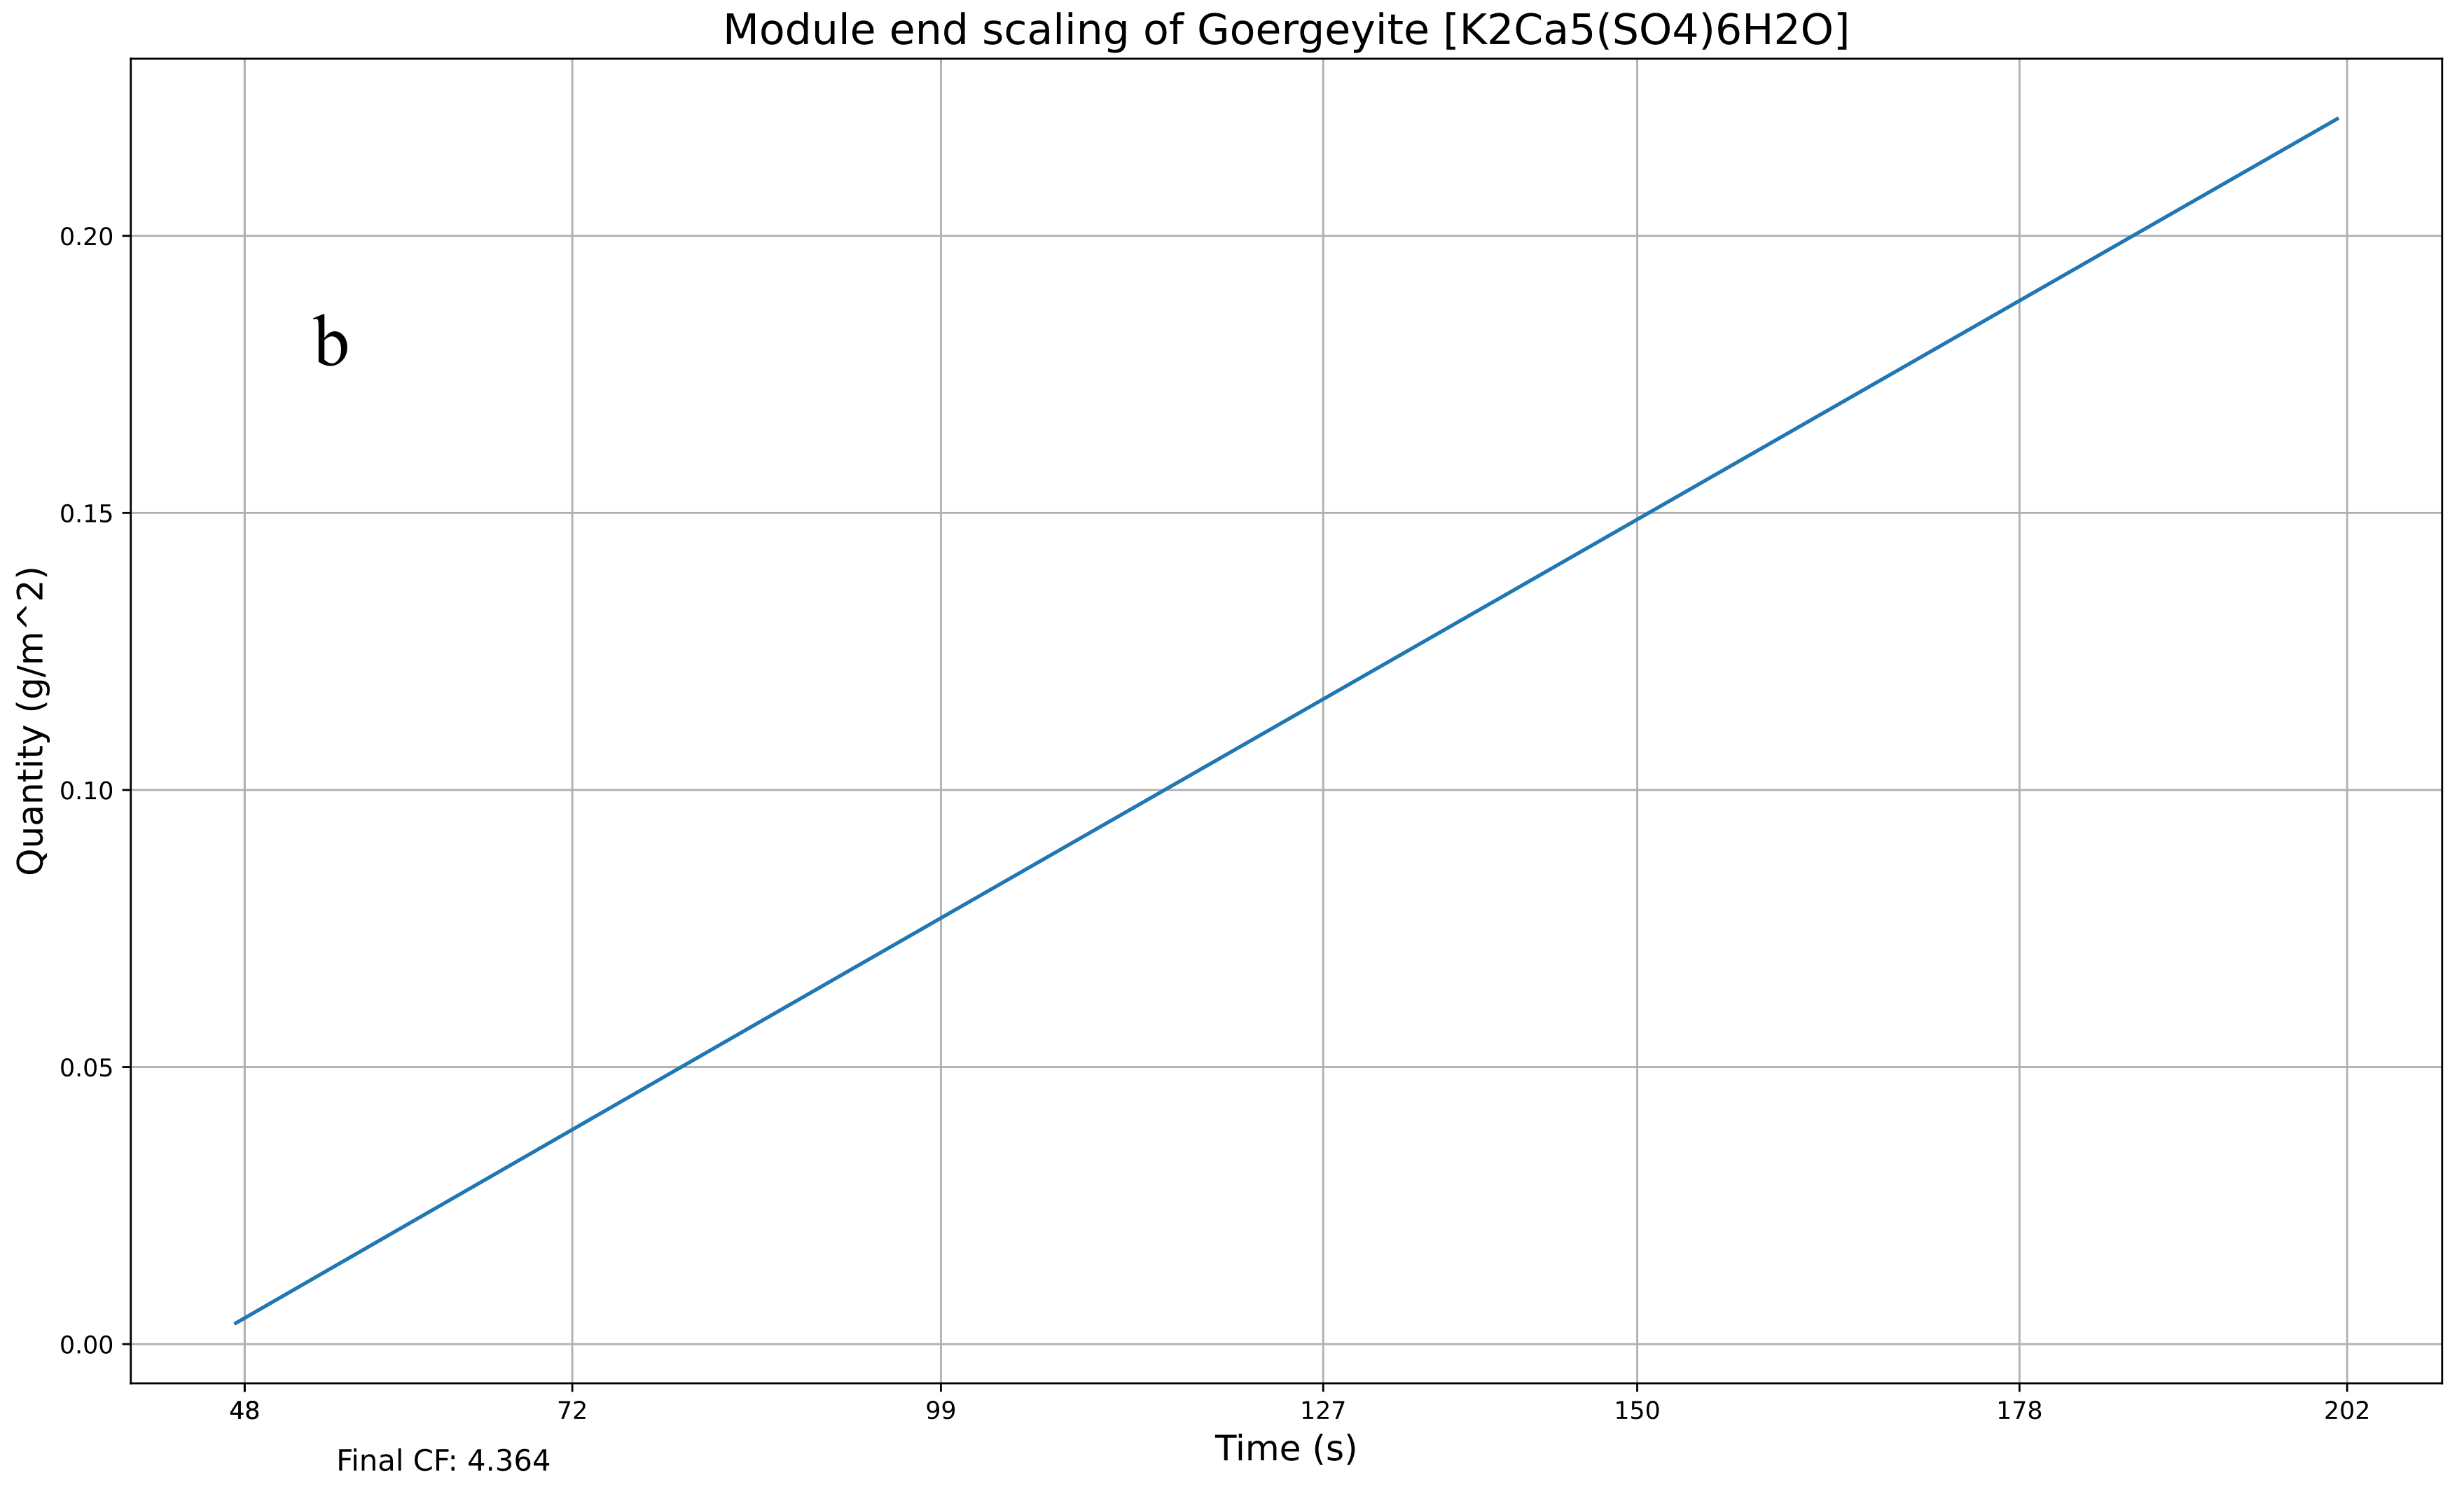
\includegraphics[width=\linewidth]{images/ROSSpy/case_studies/scaling_all_time_goergeyite.png} 
        \\ \midrule
        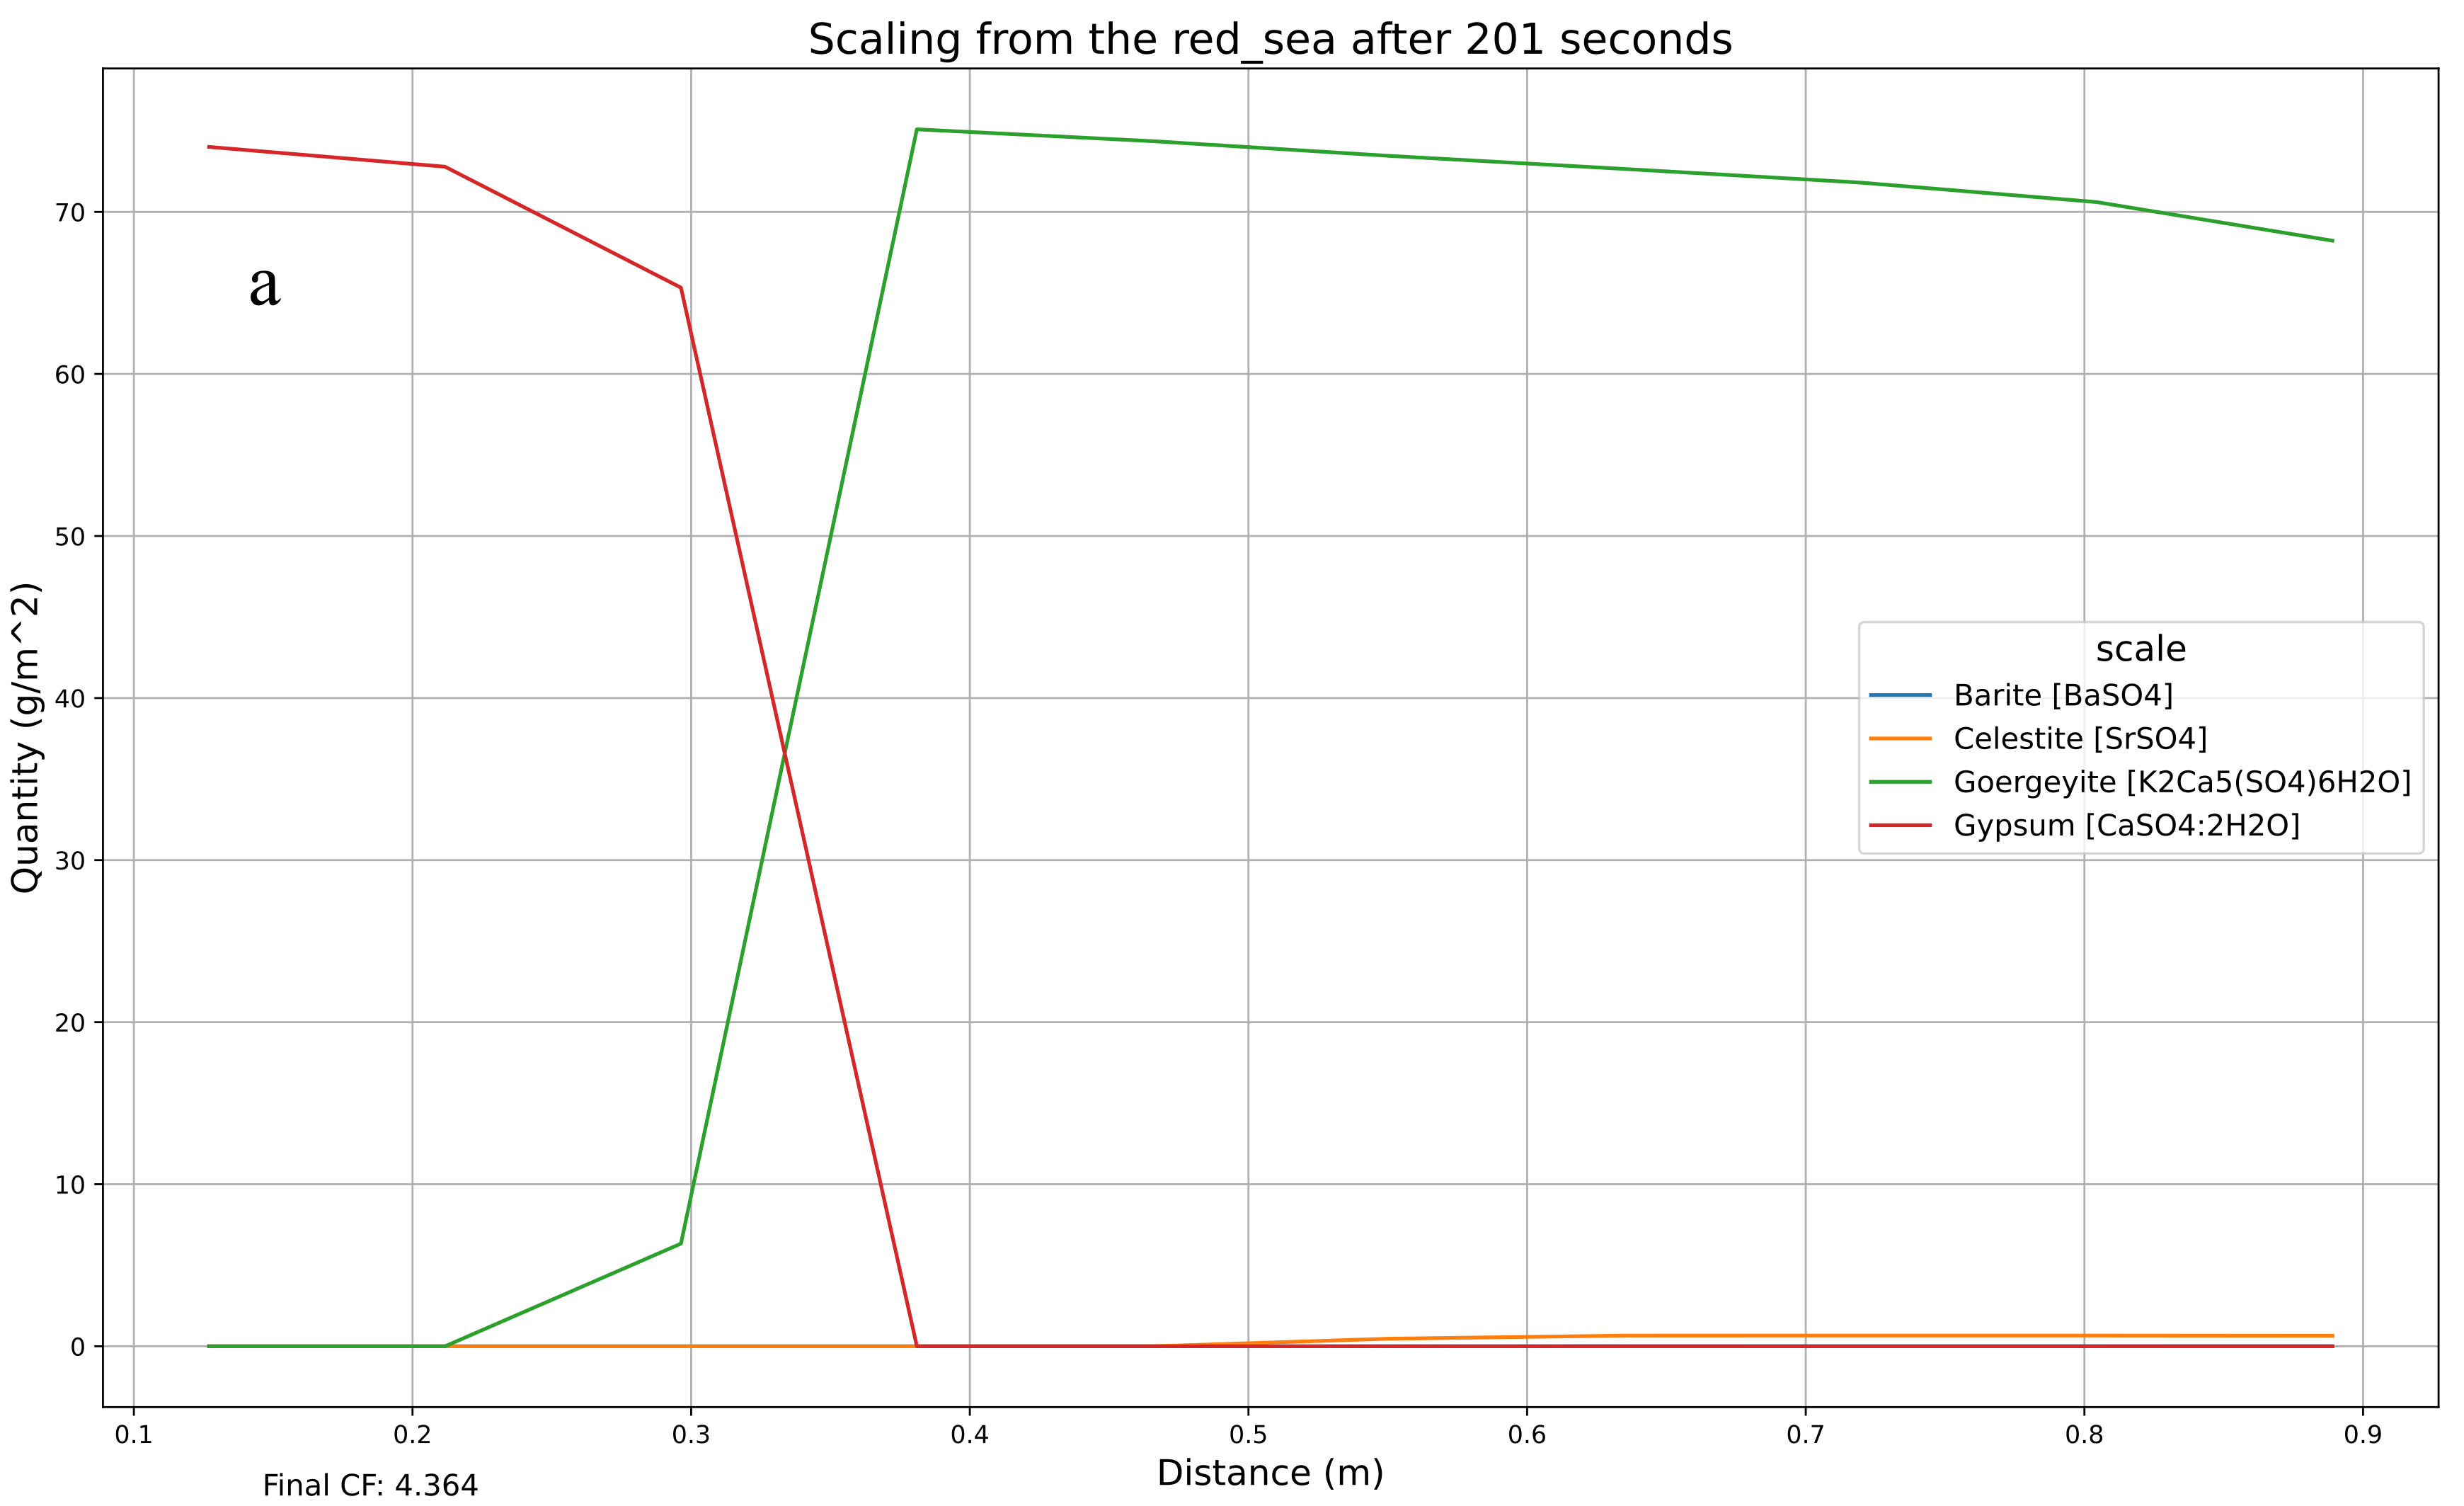
\includegraphics[width=\linewidth]{images/ROSSpy/case_studies/scaling_all_distance.png} 
    \end{tabular}
    \caption{
        Scaling while either a) slicing through time at the end distance or b) slicing  through distance at the final time. The permeate flux of the simulation is elevated to augment the scaling geochemistry for this illustration.
    }
    \label{scaling_perspectives}
\end{figure}

\subsection{Feed geochemistry}
Each of the default feed parameter files, including both natural seas and produced waters from oil wells, were evaluated with otherwise identical simulation parameters. The scaling and brine predictions differed significantly amongst these feed water sources, which are sampled in Figure \ref{feed_sources}.  

\begin{figure}[h]
    \centering
    \begin{tabular}{c|c}
        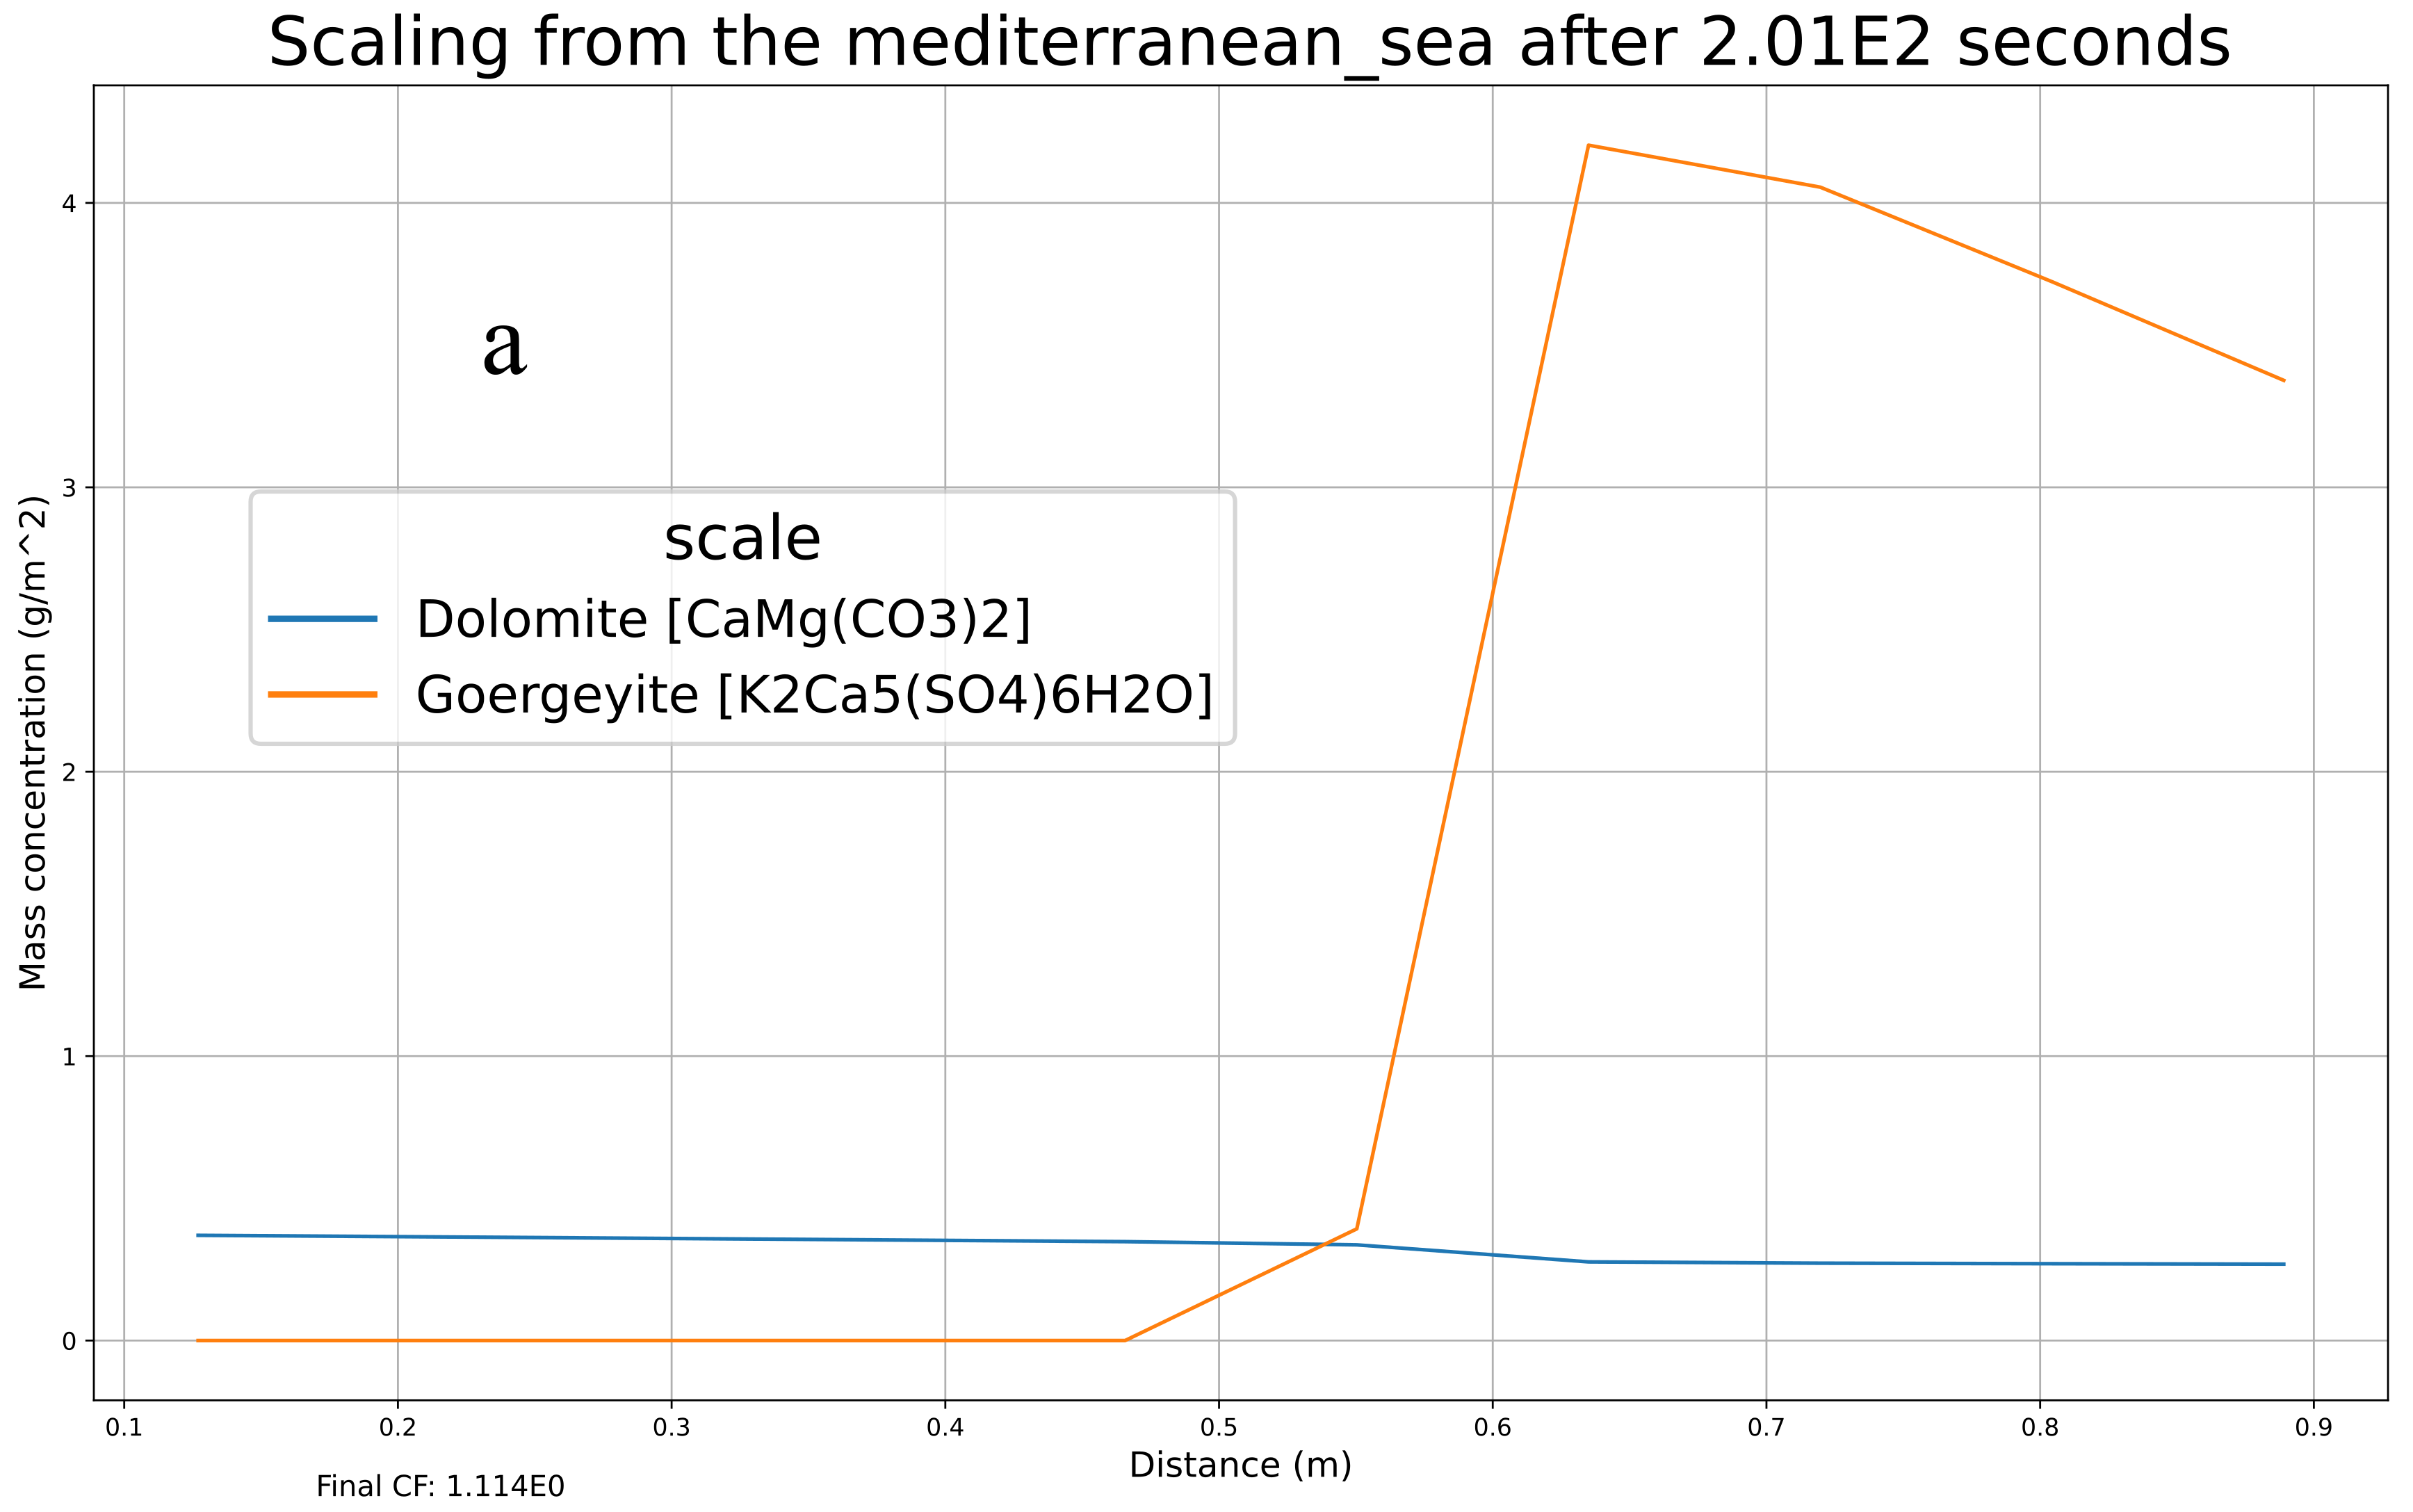
\includegraphics[width=0.49\textwidth]{images/ROSSpy/sensitivity_analyses/feed_source/Mediterranean.png} &
        \includegraphics[width=0.49\textwidth]{images/ROSSpy/sensitivity_analyses/feed_source/Palo_Duro_basin.png} \\ \midrule
        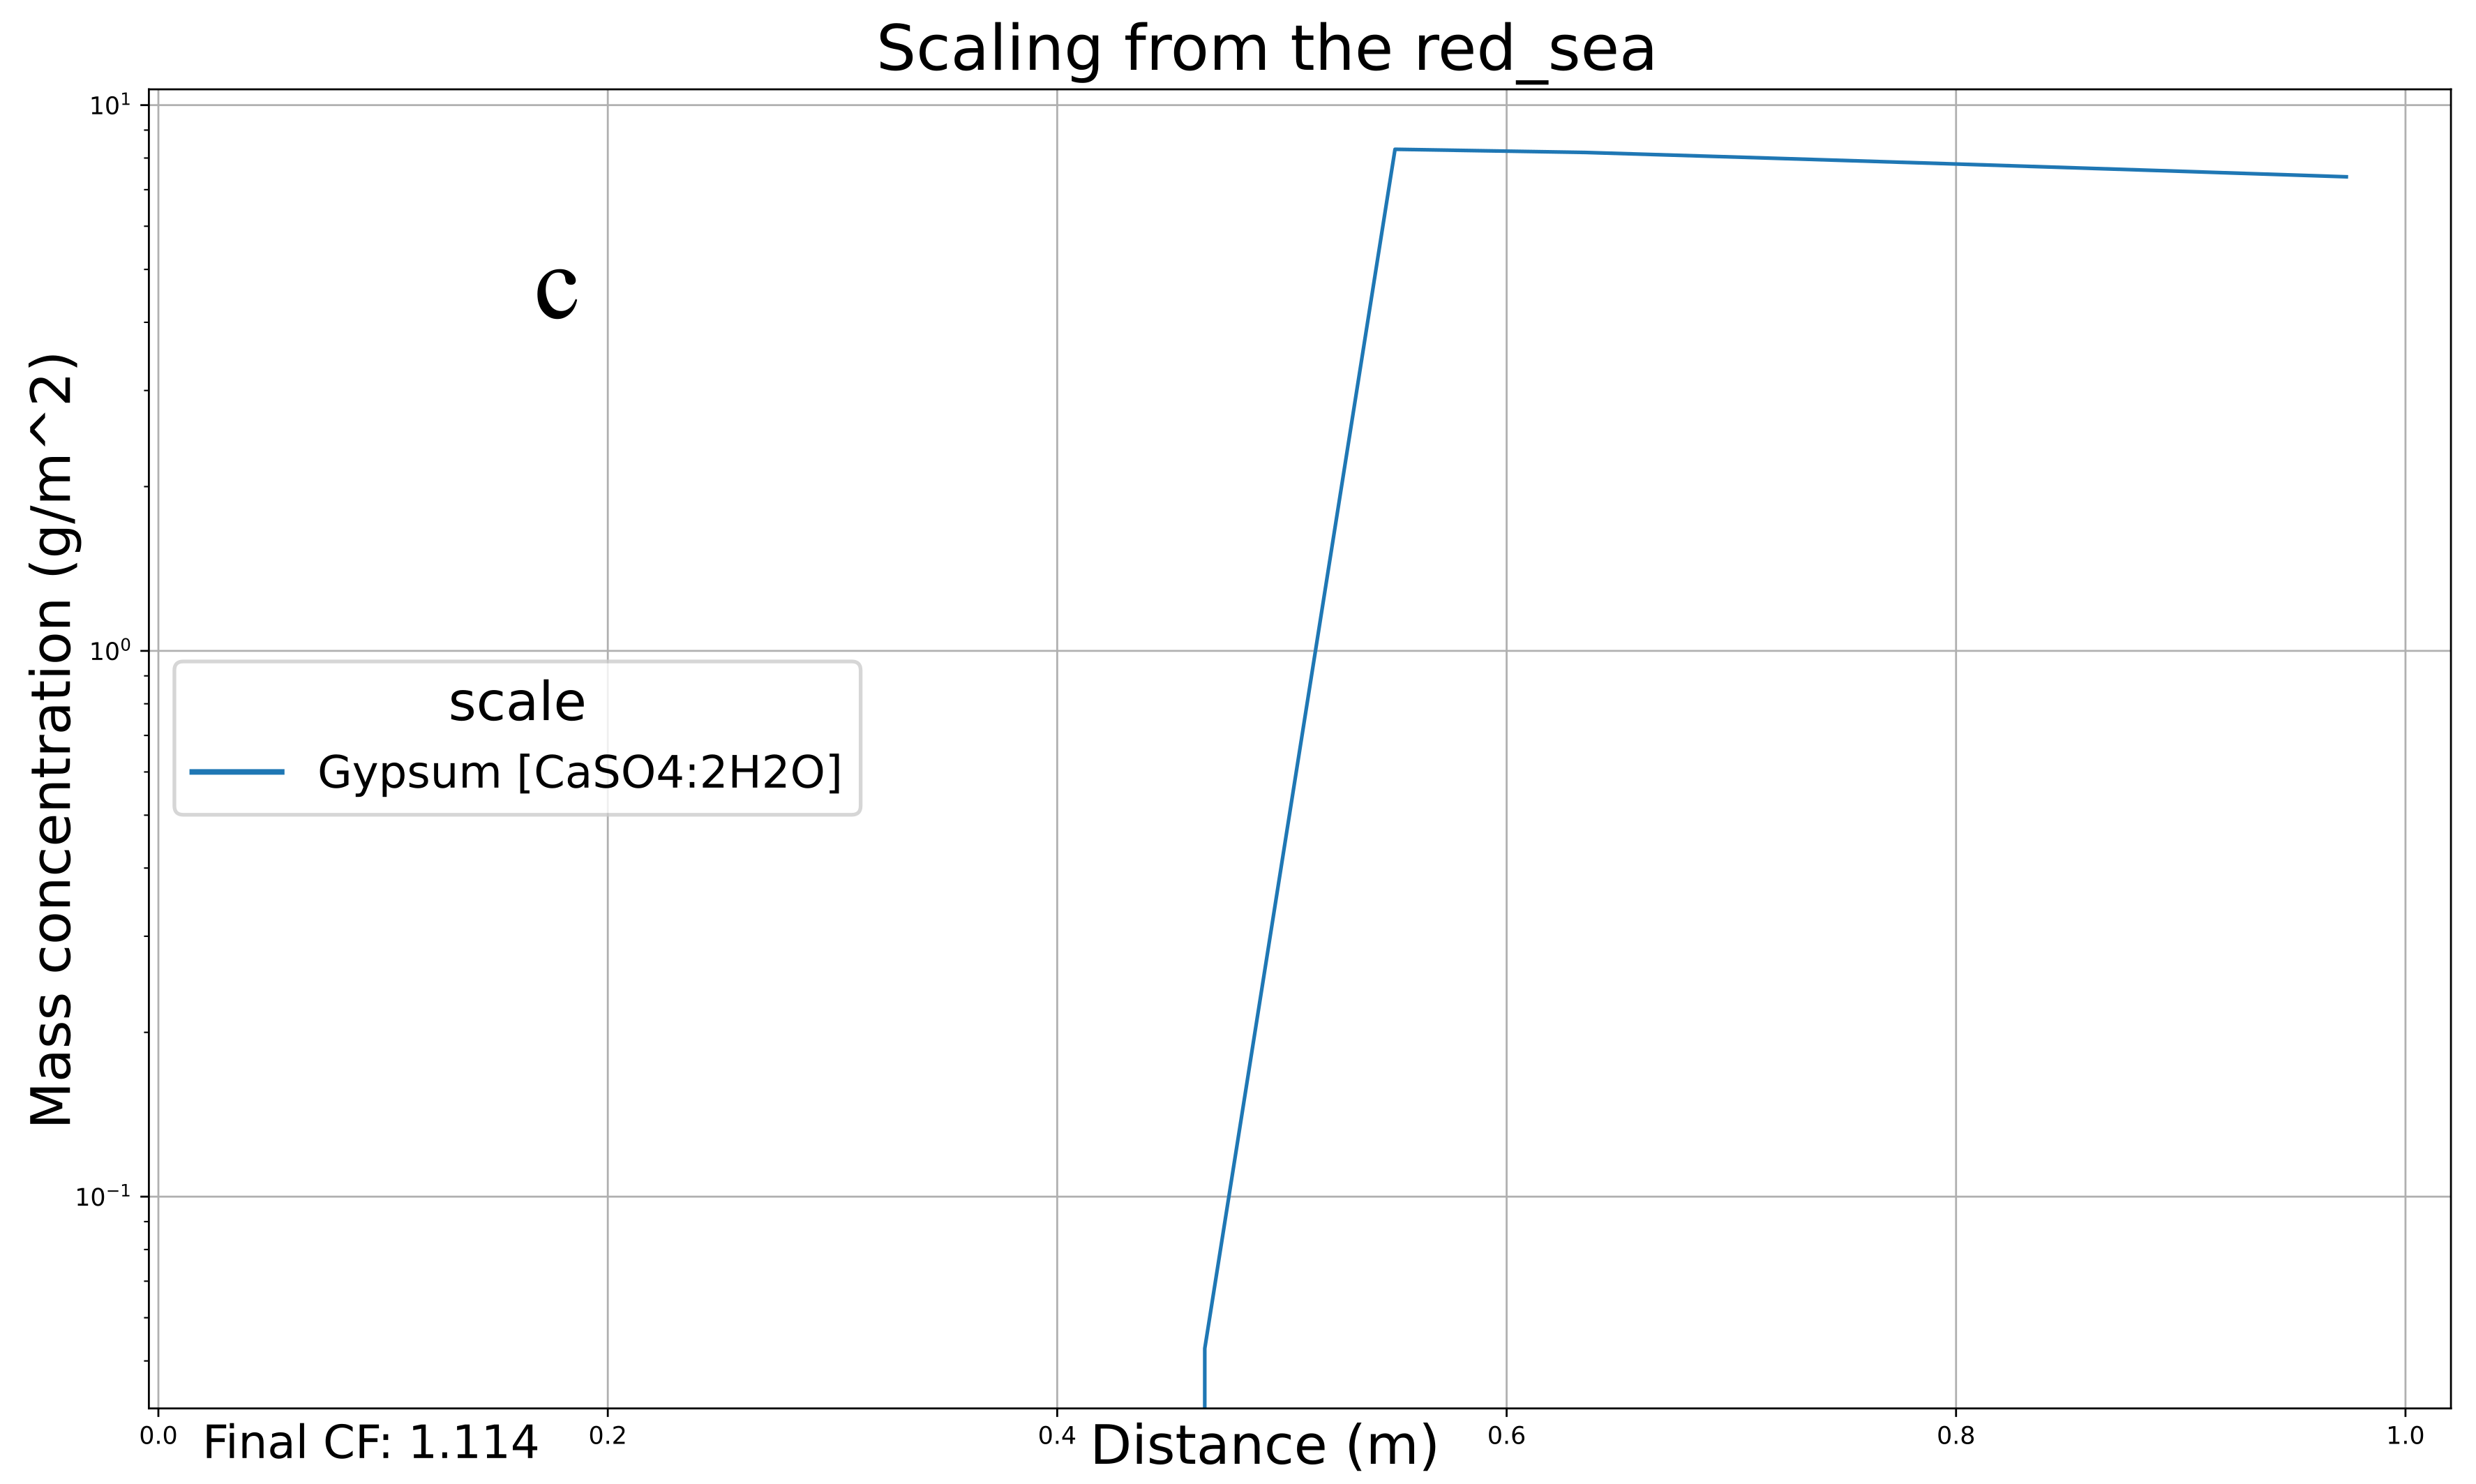
\includegraphics[width=0.49\textwidth]{images/ROSSpy/sensitivity_analyses/feed_source/Red_Sea.png} & 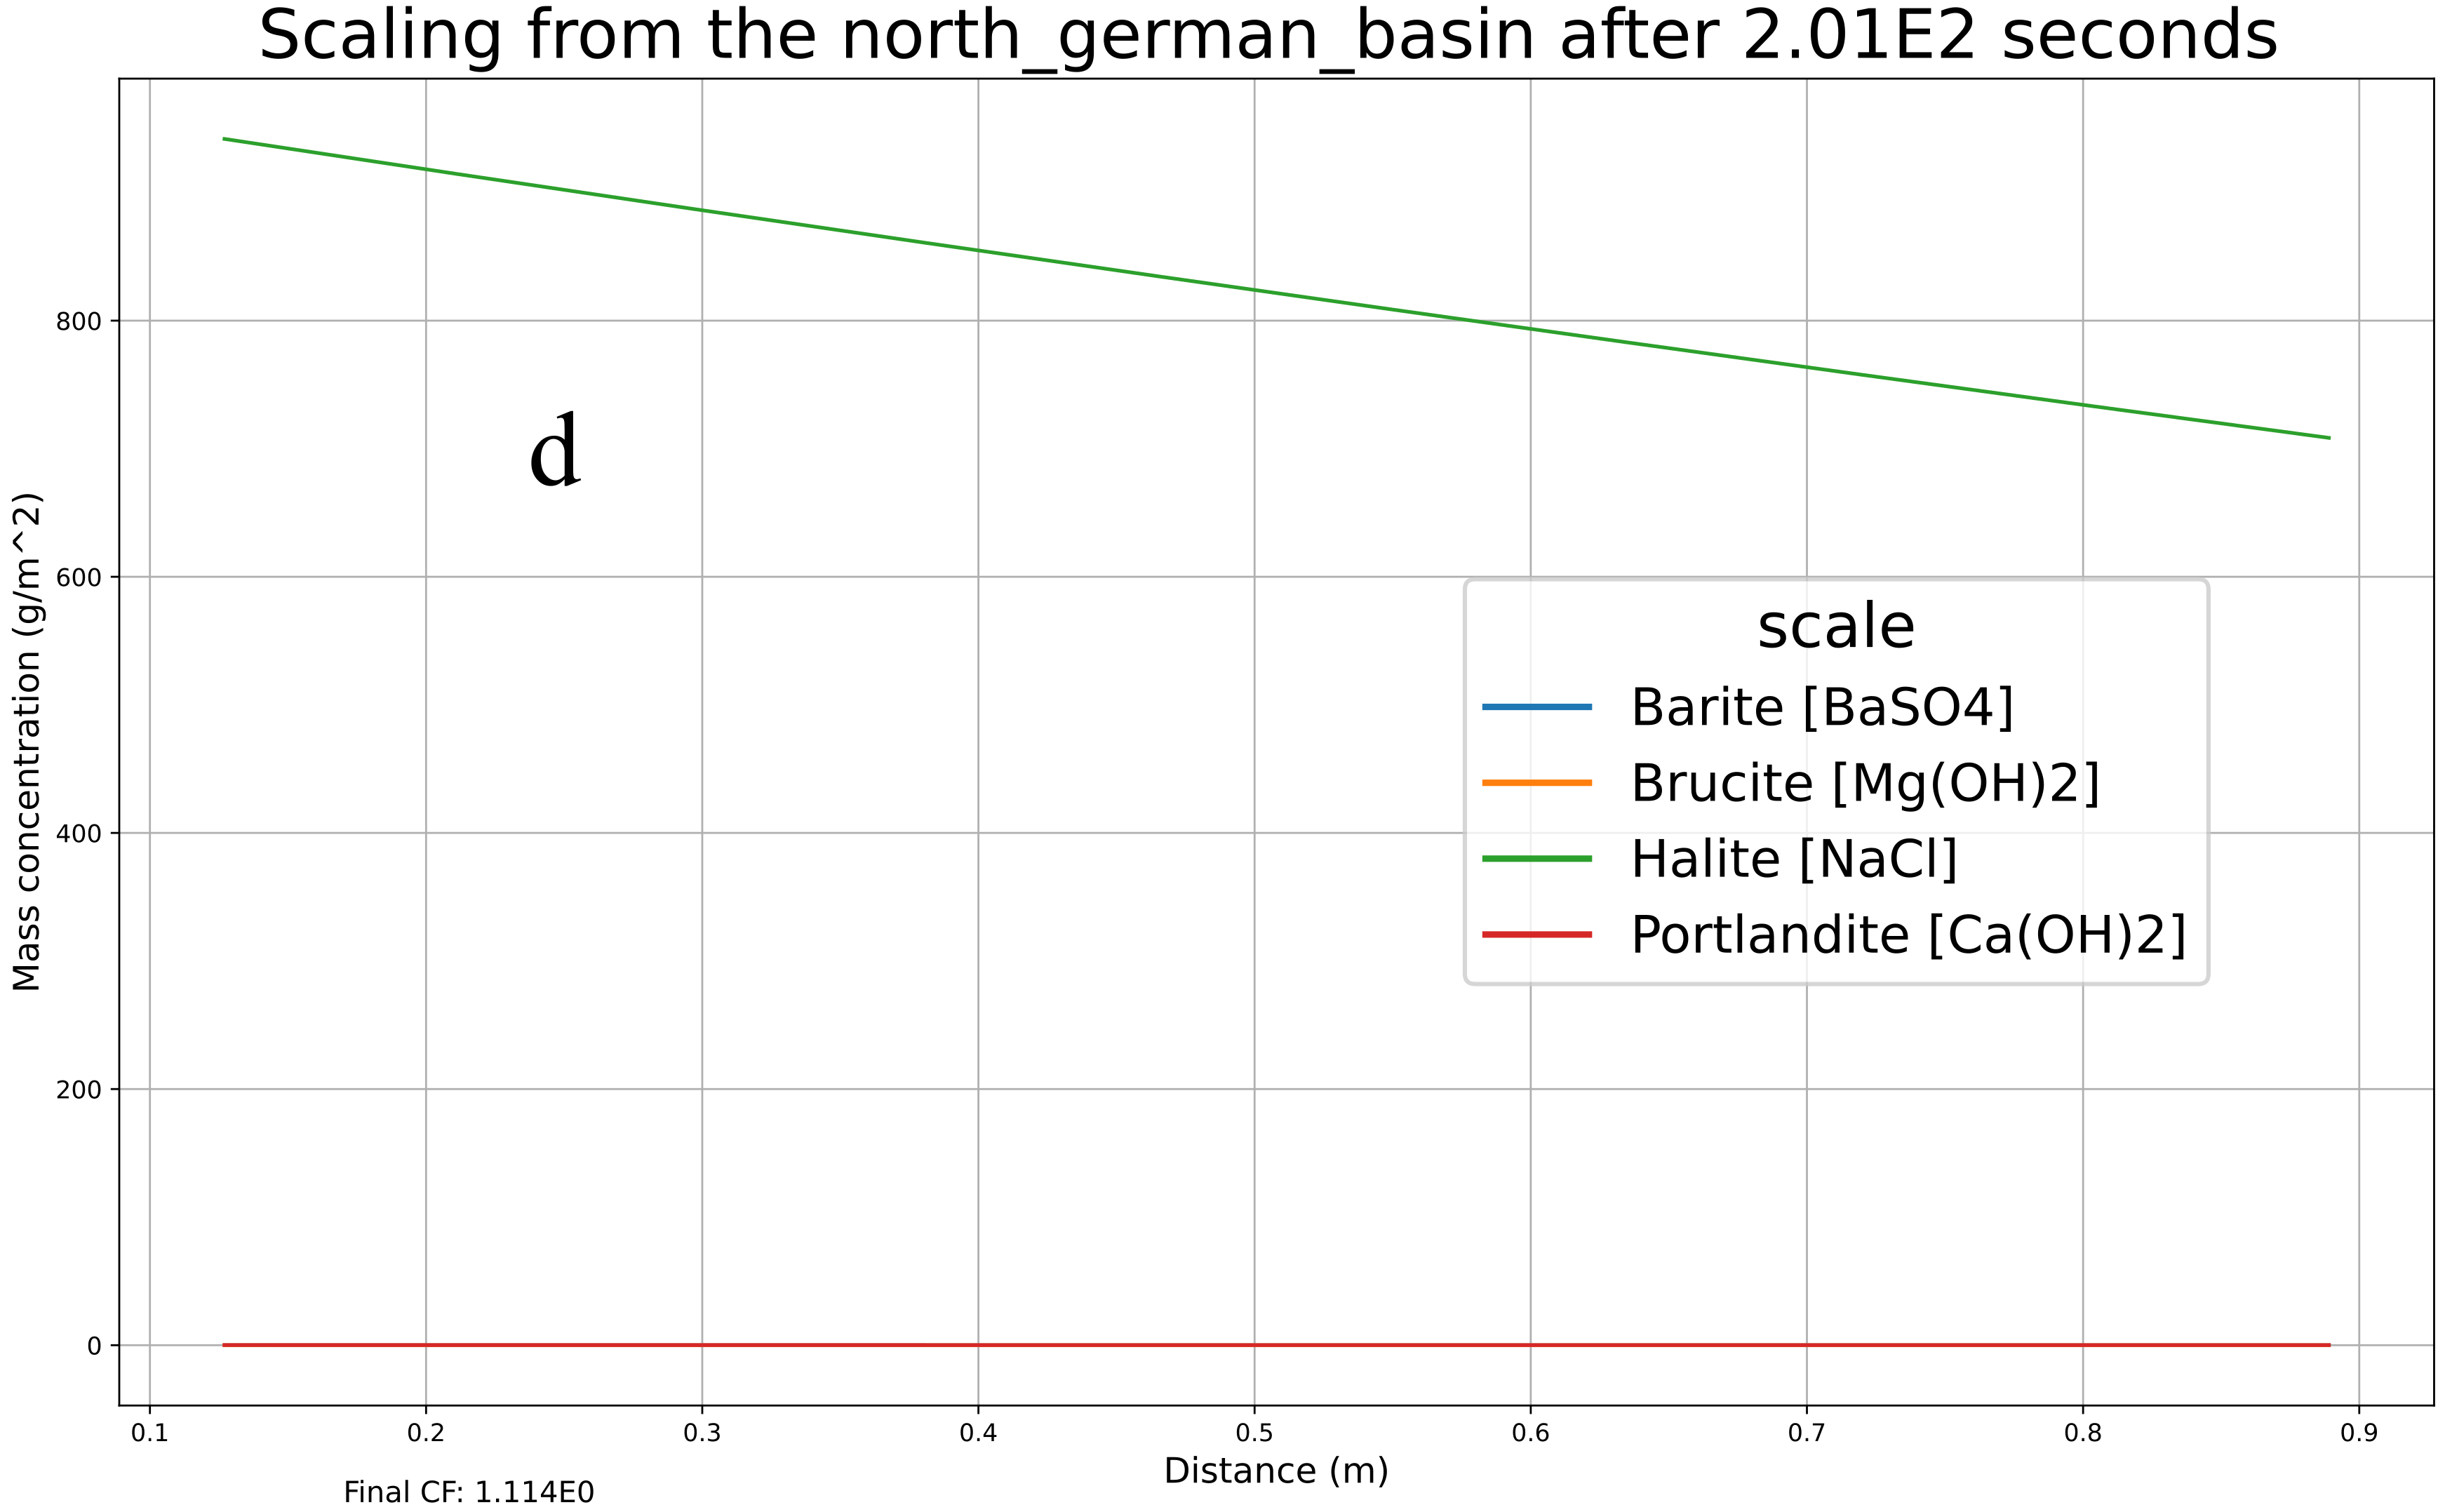
\includegraphics[width=0.49\textwidth]{images/ROSSpy/sensitivity_analyses/feed_source/German_Basin.png} \\ \bottomrule
    \end{tabular}
    \caption{
        Scaling predictions of a) the Mediterranean Sea, b) produced waters from the Palo Duro oil basin, c) the Red Sea, d) produced waters from the North German oil basin, with otherwise identical simulation parameters.
    }
    \label{feed_sources}
\end{figure}


\section{Conclusion}

A one-dimensional approximation of RO reactive transport geochemistry, executed in PHREEQC, is a practical, lightweight, and accurate approach of representing mineral scaling from RO desalination. A range of simulation applications of this model were quantitatively and qualitatively verified through its implementation as the first Python API of desalination: ROSSpy. The light-weight program is furthermore tenable for personal computers, accessible through common coding languages, and open-source for community involvement and improvement. We expect that these unique attributes of the one-dimensional model and the ROSSpy module -- e.g. rapidly designing, executing, processing, and exporting RO simulations -- will facilitate scaling research and ultimately improve the efficiency of RO desalination towards alleviating water insecurities around the world. 

\section{Funding}
This work was prepared in partial fulfillment of the requirements of the Berkeley Lab Undergraduate Research (BLUR) Program, managed by Workforce Development \& Education at the Berkeley Lab. The project was also partly funded by NSERC Discovery, MITACS Accelerate, CEWIL, and Canada Summer Jobs. 

% Acknowledgements section
\section{acknowledgement}
The authors thank Ethan Sean Chan for his technical assistance in developing iROSSpy. 